%%% aQGC %%%
\chapter{Interpretation with Effective Field Theory}
\label{chap:aQGC}

The previously obtained results are interpreted to the limits on the EFT operators. The setups for the EFT interpretation and the systematics treatments are described in this chapter.
\section{aQGC signals for EFT interpretation}
In the EFT interpretation approach, the dimension-8 operators are added to the standard model Lagrangian as described in Chapter~\ref{}. 
The EFT can be parameterized by the effective Lagrangian:
\begin{equation}
  \mathcal{L}=\mathcal{L}_{sm}+\sum_{i}\frac{f_i}{\Lambda^{2}}\mathcal{L}_i+\sum_{n}\frac{f_n}{\Lambda^{4}}\mathcal{L}_n
\end{equation}
where $\mathcal{L}$ represent possible dim-6 of dim-8 operators.
The $f_i$ corresponds to the Wilson coefficient. The new scale $\Rambda$ represents the cutoff scale, which is the energy scale where the added operators are effective up to this scale. 
The odd dimension operators violate lepton and baryon number conservation and are ignored here.
Dimension-6 operators can introduce charged aTGCs, while dimension-8 operators are the lowest order which can induce the aQGC, both of which can contribute to the VBS process.
Due to the existing tight constraints of dimension-6 operators from inclusive diboson measurements, only dimension-8 operators will be discussed.
The matrix element from the whole Lagrangian including the additional operators can be linearly parametrized as:
\begin{equation}
\left|A_{\mathrm{SM}}+\sum_{i} \frac{f_{i}}{\Lambda^{4}} A_{i}\right|^{2}=\left|A_{\mathrm{SM}}\right|^{2}+\sum_{i} 2 \frac{f_{i}}{\Lambda^{4}} \operatorname{Re}\left(A_{i}^{*} A_{\mathrm{SM}}\right)+\sum_{i} \frac{f_{i}^{2}}{\Lambda^{8}}\left|A_{i}\right|^{2}+\sum_{i \neq j} 2 \frac{f_{i} f_{j}}{\Lambda^{8}} \operatorname{Re}\left(A_{i}^{*} A_{j}\right)
\label{eqn:eftamplitude}
\end{equation}
The first term of the equation~\ref{eqn:eftamplitude} represents the standard model (SM) contribution. The second and the third term represents the contributions from the interference term between the EFT and the SM operator and the purely EFT operator, respectively. Each terms are referred to as quadratic (QUAD) term and the interference (INT) term. The last term is the cross term between the EFT operators, which is ignored in this analysis for the simplicity and the consistency with the other aQGC search analyses. The Wilson coefficient $f_i$ and the cut-off scale $\Rambda$ cannot be separated, therefore the constraints are always given on their ratio, $f_i/\Rambda^4$.

The QUAD term and the INT terms are produced as the separated signal samples. These two terms can be combined into single POI by adding the postprocessing procedure in the fitting framework to parameterize as $\mu_{QUAD} = \mu_{INT}^2$.

For the dimension-8 operators, Eboli model is used as described in Chapter~\ref{}.
The cross sections for these aQGC signal samples are produced with MadGraph5\_aMC@NLO v2.3.3, plus \PYTHIA8~\cite{Sjostrand:2007gs} for fragmentation, and the \textsc{NNPDF30LO} PDF set~\cite{Ball:2012cx} similar as the EW signals. (\textcolor{blue}{really?})


\section{Binned significance study}

The 2-dimensional binned significance using $m_{VV}$ and RNNScore as discriminant is studied in \tlep channel.

Figures~\ref{fig:2lepaQGCshapeMVV} and \ref{fig:2lepaQGCshapeRNN} show the $m_{VV}$ and RNNScore distributions for some aQGC samples, compared with the SM electroweak signal and the other background processes.
$m_{VV}$ distributions for aQGC signals are significantly higher than the SM electroweak signal and the other background.
The RNNScore distributions for aQGC samples are found to be similar to the one for the SM electroweak signals.
The RNN trained for the SM electroweak signal is also useful to separate aQGC signals from the other background processes.

\begin{figure}[ht]
    \centering
    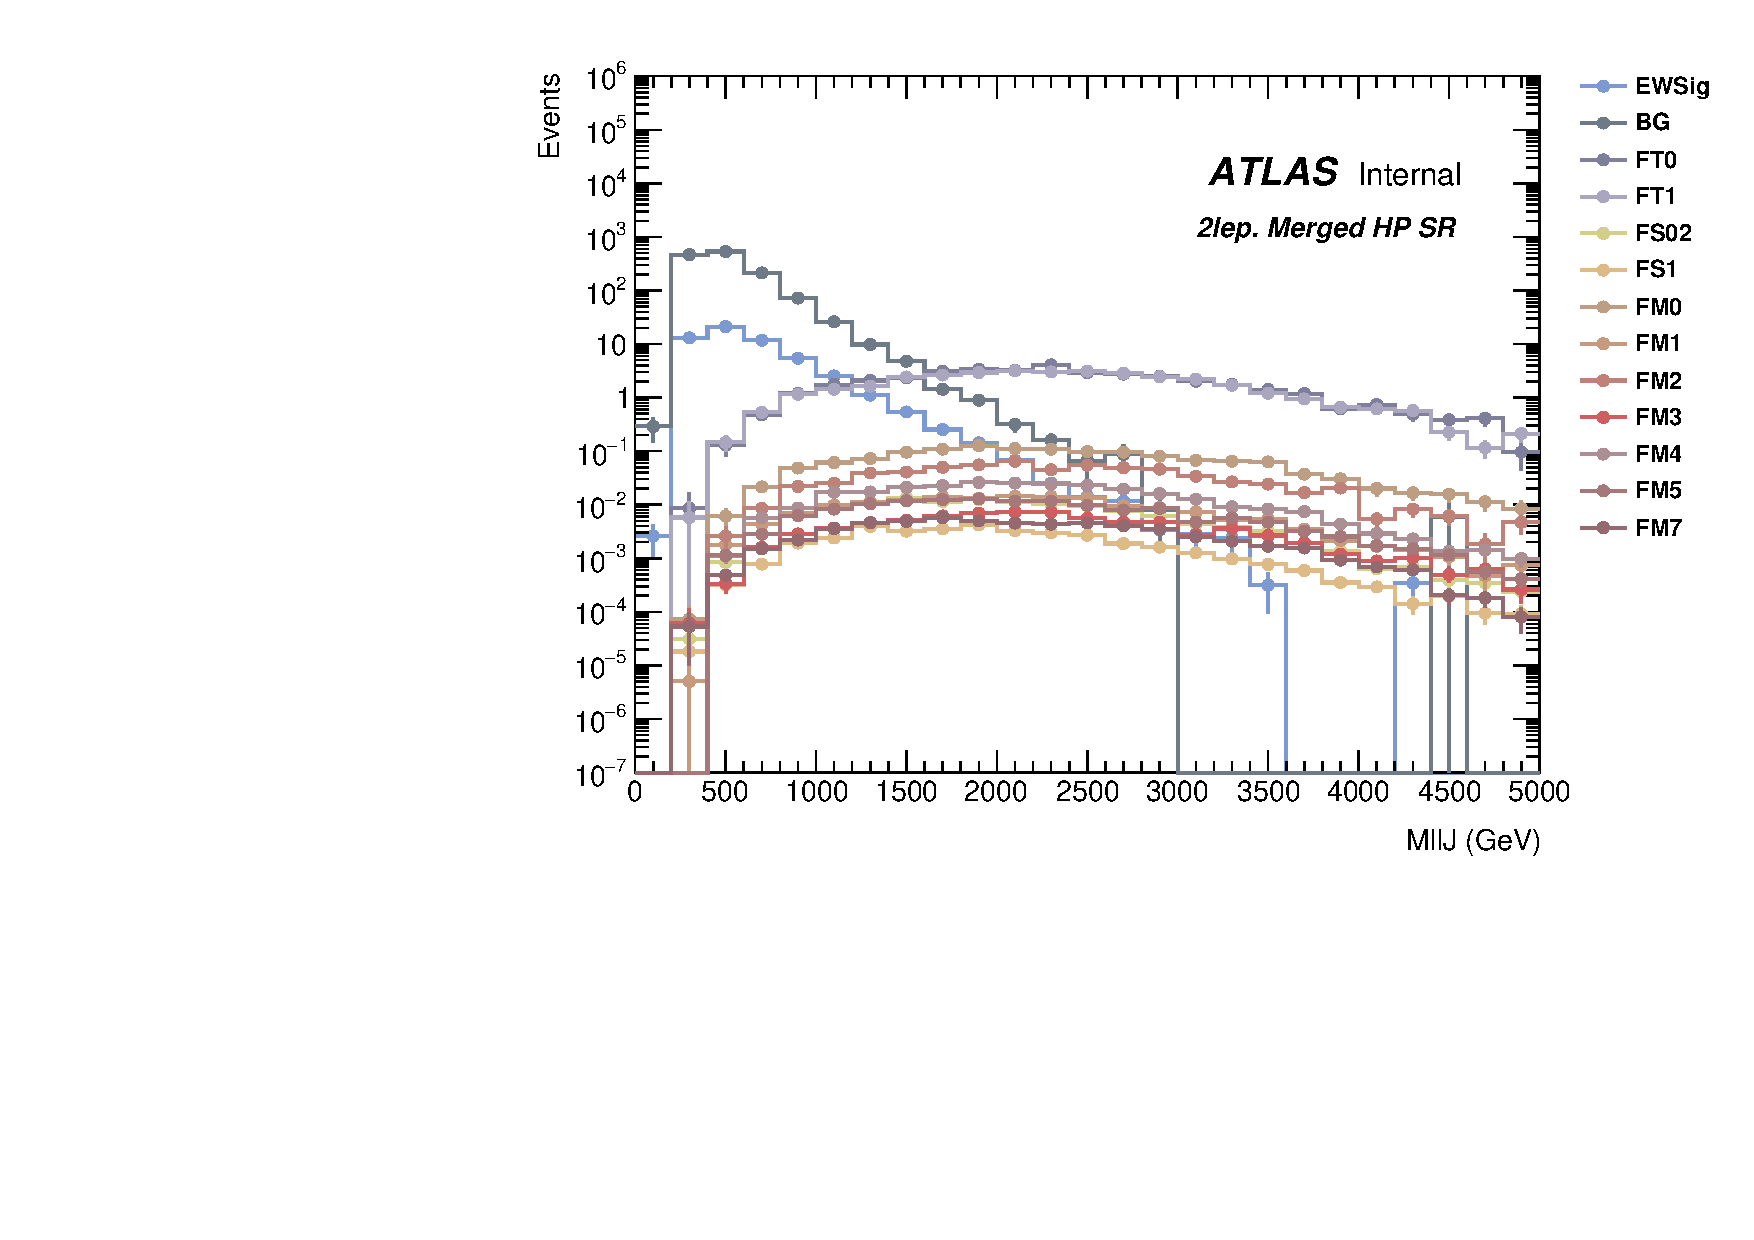
\includegraphics[width=0.45\textwidth]{figures/aQGC/MllJ_SR_HP_aQGC.pdf}
    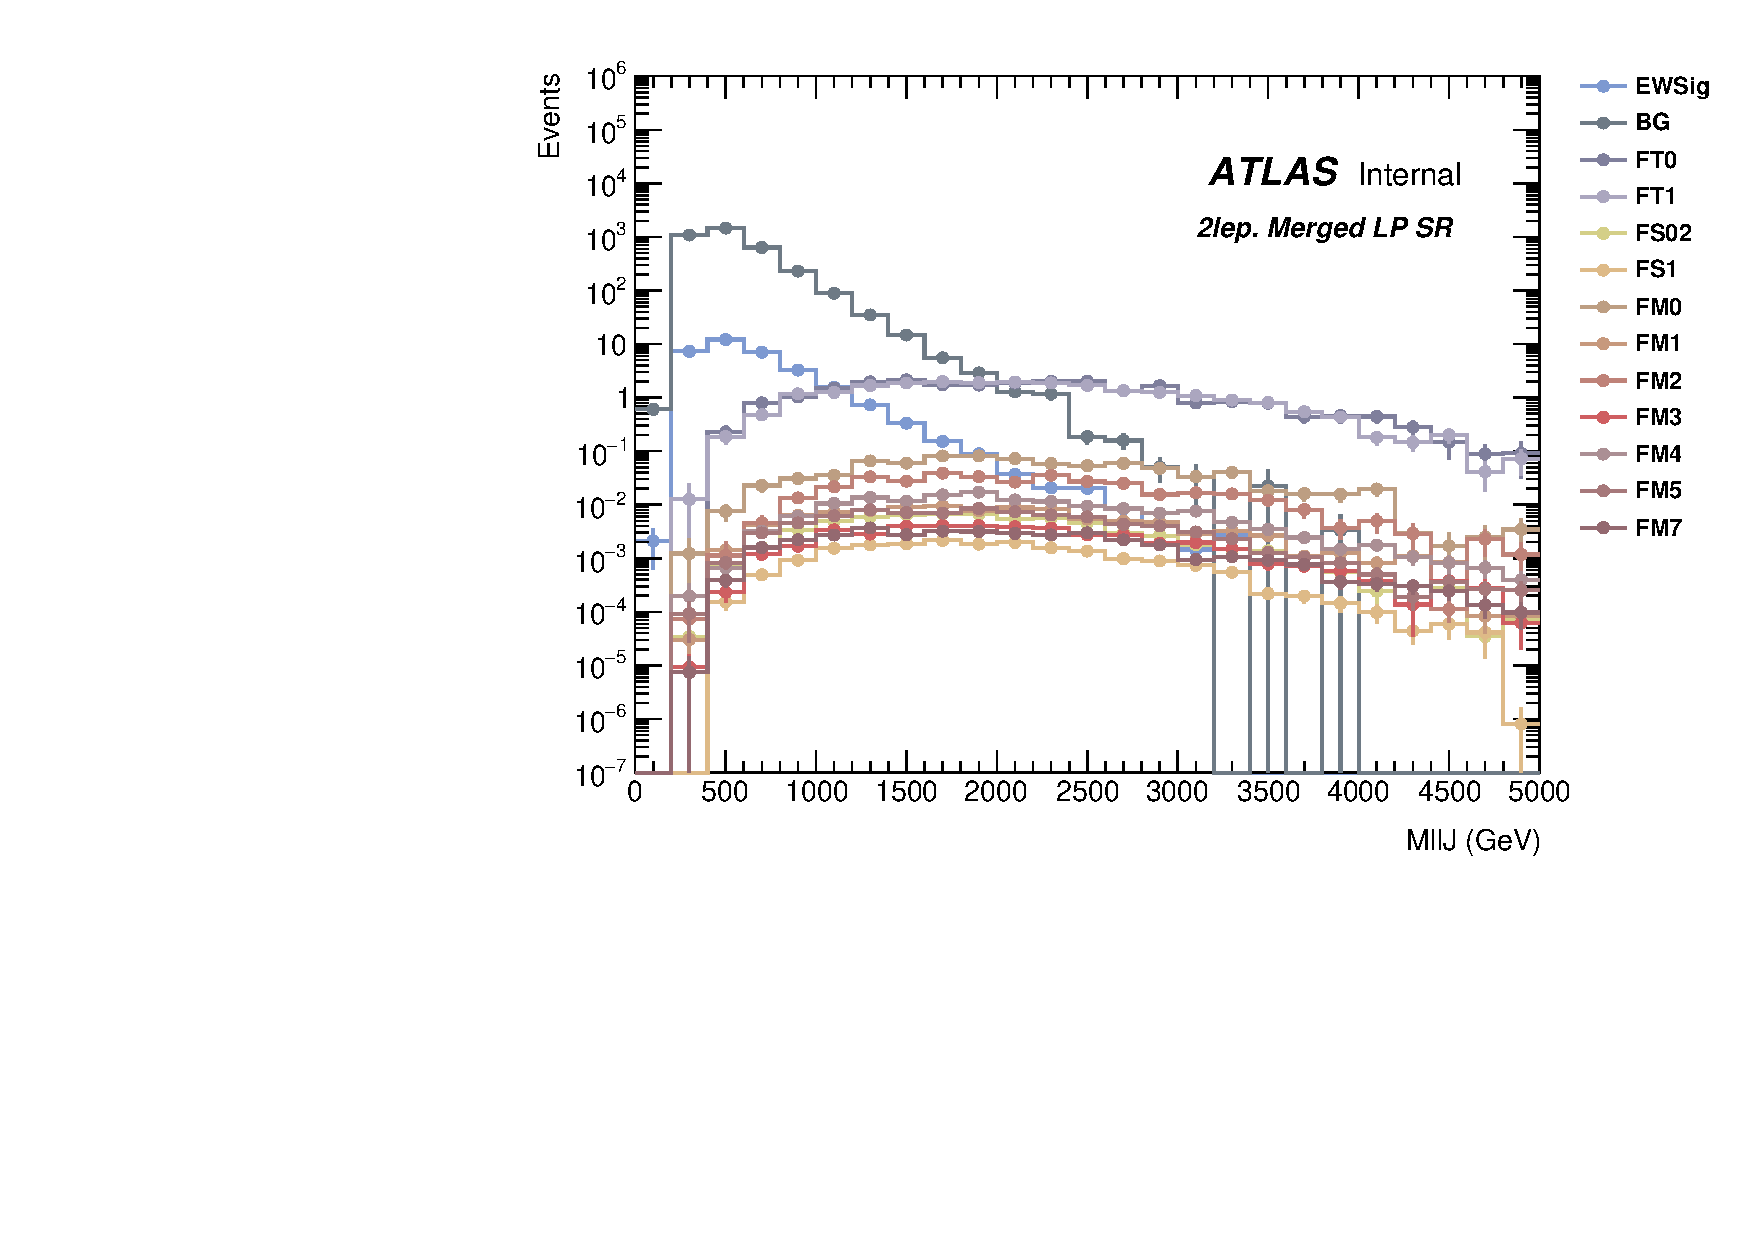
\includegraphics[width=0.45\textwidth]{figures/aQGC/MllJ_SR_LP_aQGC.pdf}
    \caption{$m_{VV}$ shape distribution of each Wilson coefficient in Merged Signal regions. Only quadratic terms are shown.}
    \label{fig:2lepaQGCshapeMVV}
\end{figure}

\begin{figure}[ht]
    \centering
    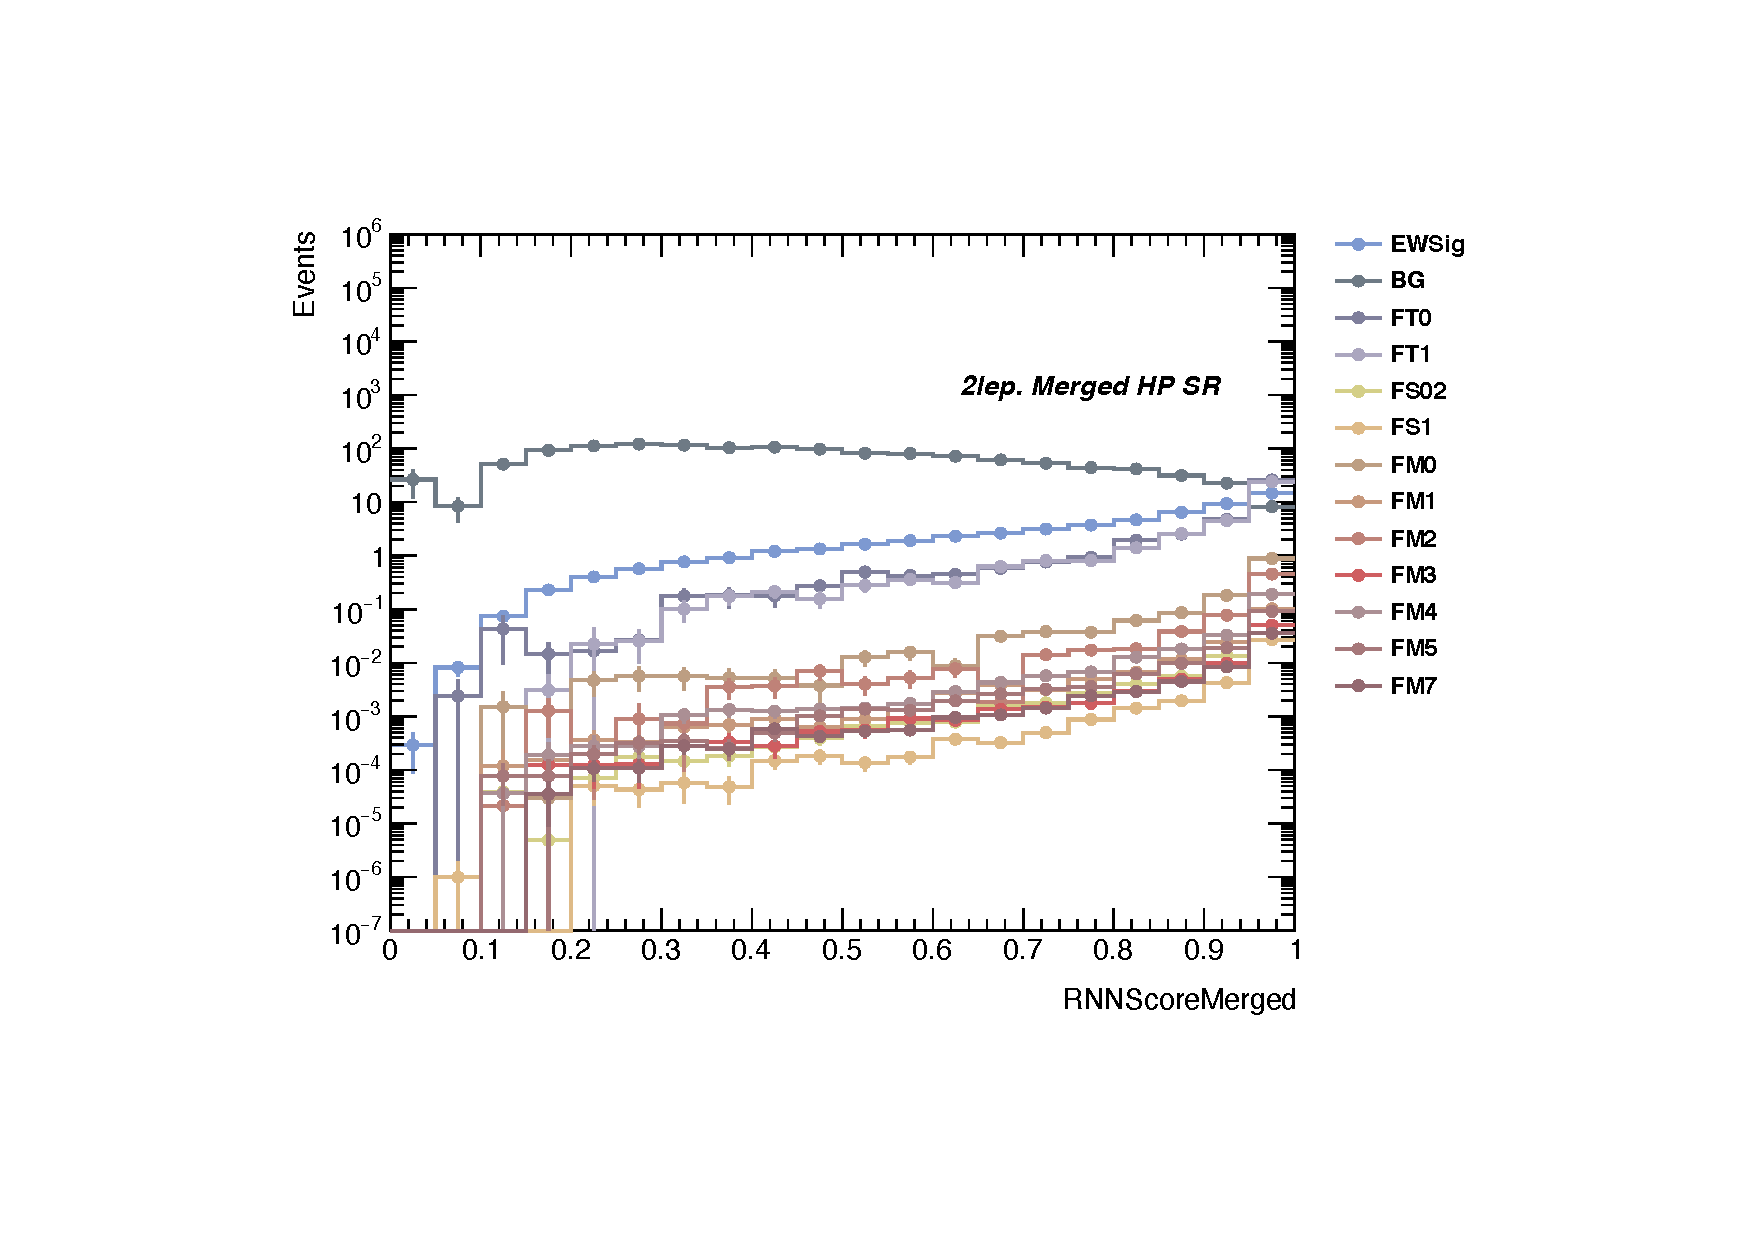
\includegraphics[width=0.45\textwidth]{figures/aQGC/RNNScoreMerged_SR_HP_aQGC.pdf}
    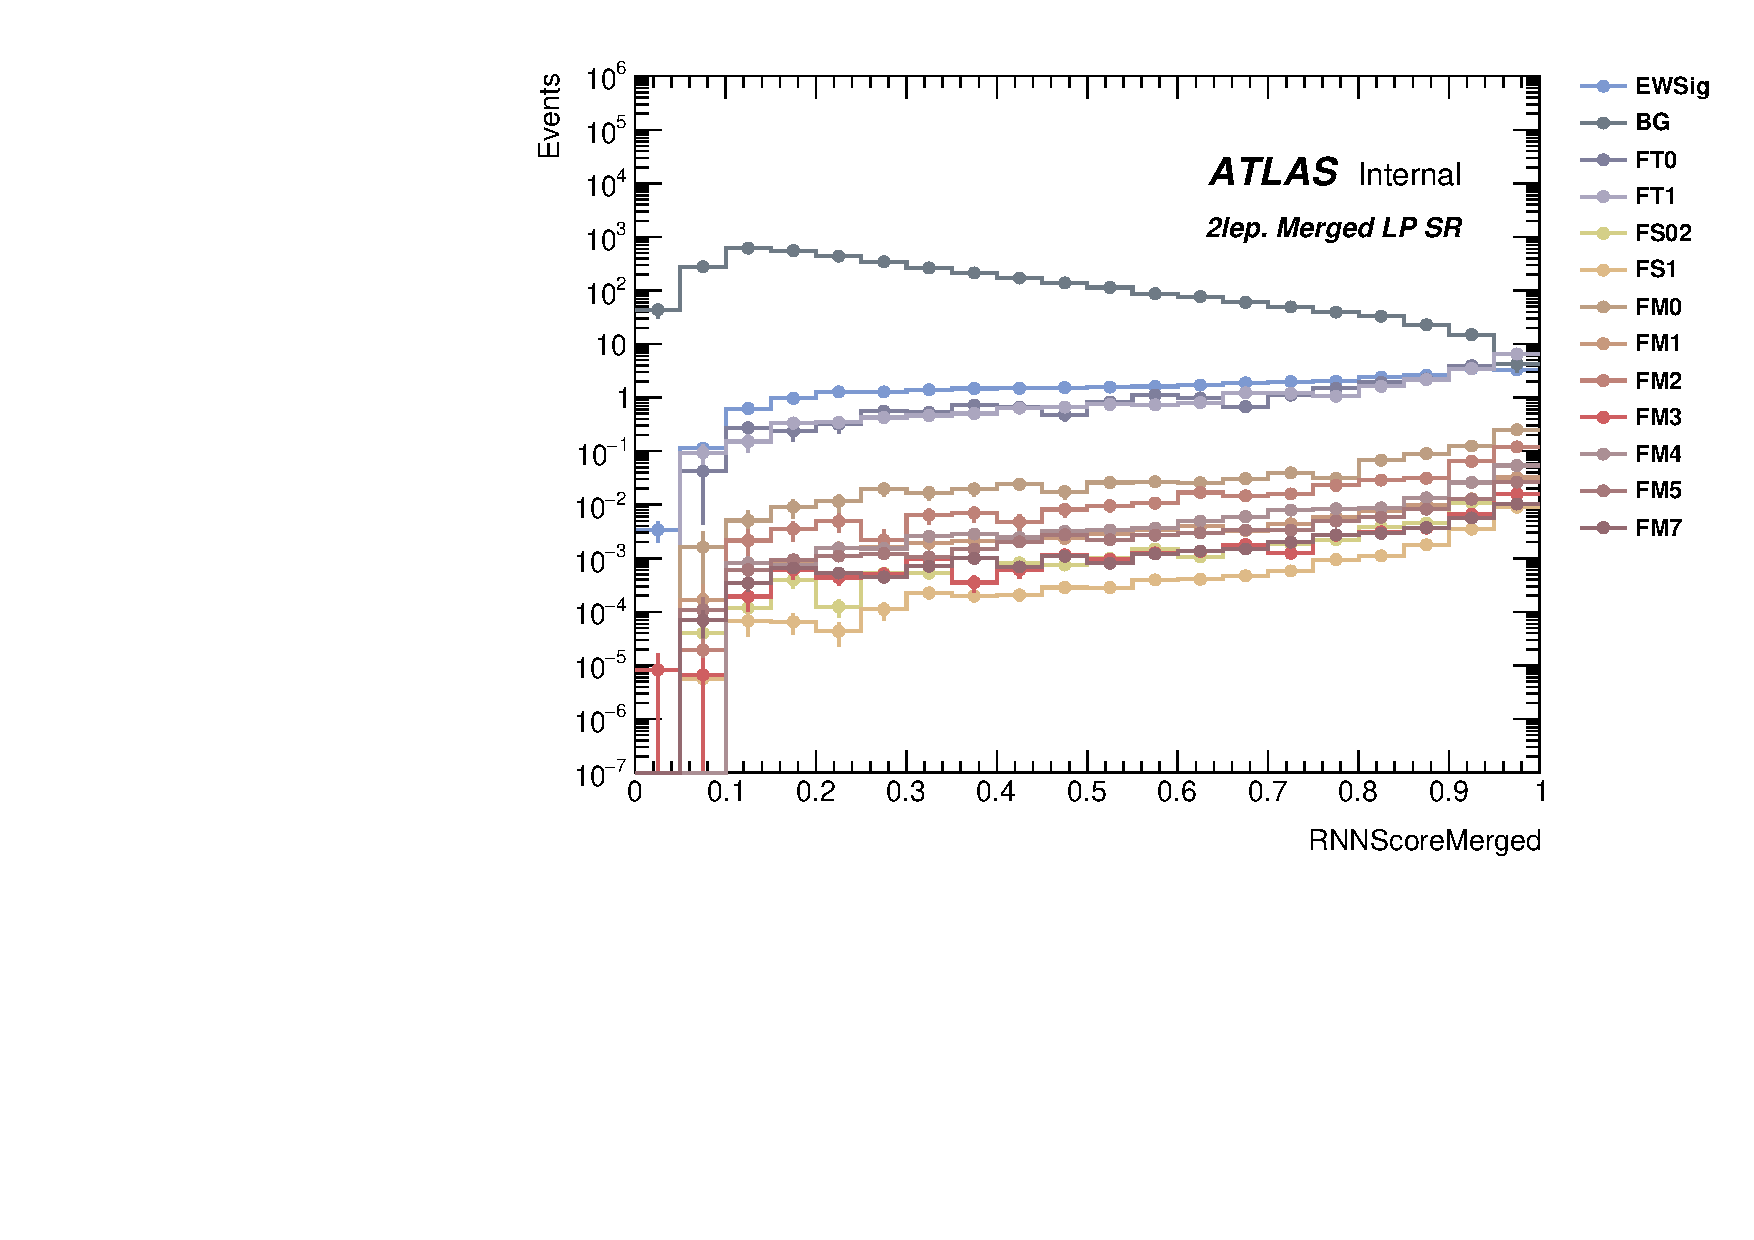
\includegraphics[width=0.45\textwidth]{figures/aQGC/RNNScoreMerged_SR_LP_aQGC.pdf}
    \caption{RNN score shape distribution of each Wilson coefficient in Merged Signal regions. Only quadratic terms are shown.}
    \label{fig:2lepaQGCshapeRNN}
\end{figure}

The significance considering both $m_{VV}$ and RNNSCore distributions is tested here.
The binned significance defined as:
%
\begin{eqnarray*}
  Z = \sqrt{\sum_{bins}\left[2(s + b)ln\left(\frac{(s + b)(b+\sigma^2_{b})}{b^2+(s+b)\sigma^2_{b}}\right) - \frac{b^2}{\sigma^2_{b}}ln\left(1+\frac{\sigma^2_{b}s}{b(b+\sigma^2_{b})}\right)\right]} \\
\end{eqnarray*}
%
is used in this study.
The $s$ here refers to the number of the aQGC signal for the given Wilson coefficient.
The $b$ includes the SM electroweak signals and the other backgrounds (like Z+jets, ttbar, Diboson).
The fractional systematic uncertainty $\sigma_{b} = 0.2$ is assumed.

Two approaches are tested.
One is to use the $m_{VV}$ distribution for the binned significance definition, after the cut on the RNNScore.
The other is to use the RNNScore distribution for the binned significance calculation, after the cut on the $m_{VV}$.

Figure~\ref{fig:2lepaQGCBinnedSigMVV} shows the binned significance using $m_{VV}$ distribution,
as functions of the cut thresholds of RNNSCore and $\mathrm{M}_{tagjj}$.
No cuts on RNNScore and $\mathrm{M}_{tagjj}$ are preferred, in particular for the FT0 term.

Figure~\ref{fig:2lepaQGCBinnedSigRNN} shows the binned significance using RNNScore distribution
as functions of the cut thresholds for $m_{VV}$ and $\mathrm{M}_{tagjj}$.
It is preferred to apply the cut on $m_{VV}$ if we want to use RNNScore as the discriminant.

The significance value for each Wilson coefficient term is summarized in tables~\ref{tab:2lep_HPSR_MVV} and \ref{tab:2lep_HPSR_RNN}.

\begin{figure}[ht]
    \centering
    	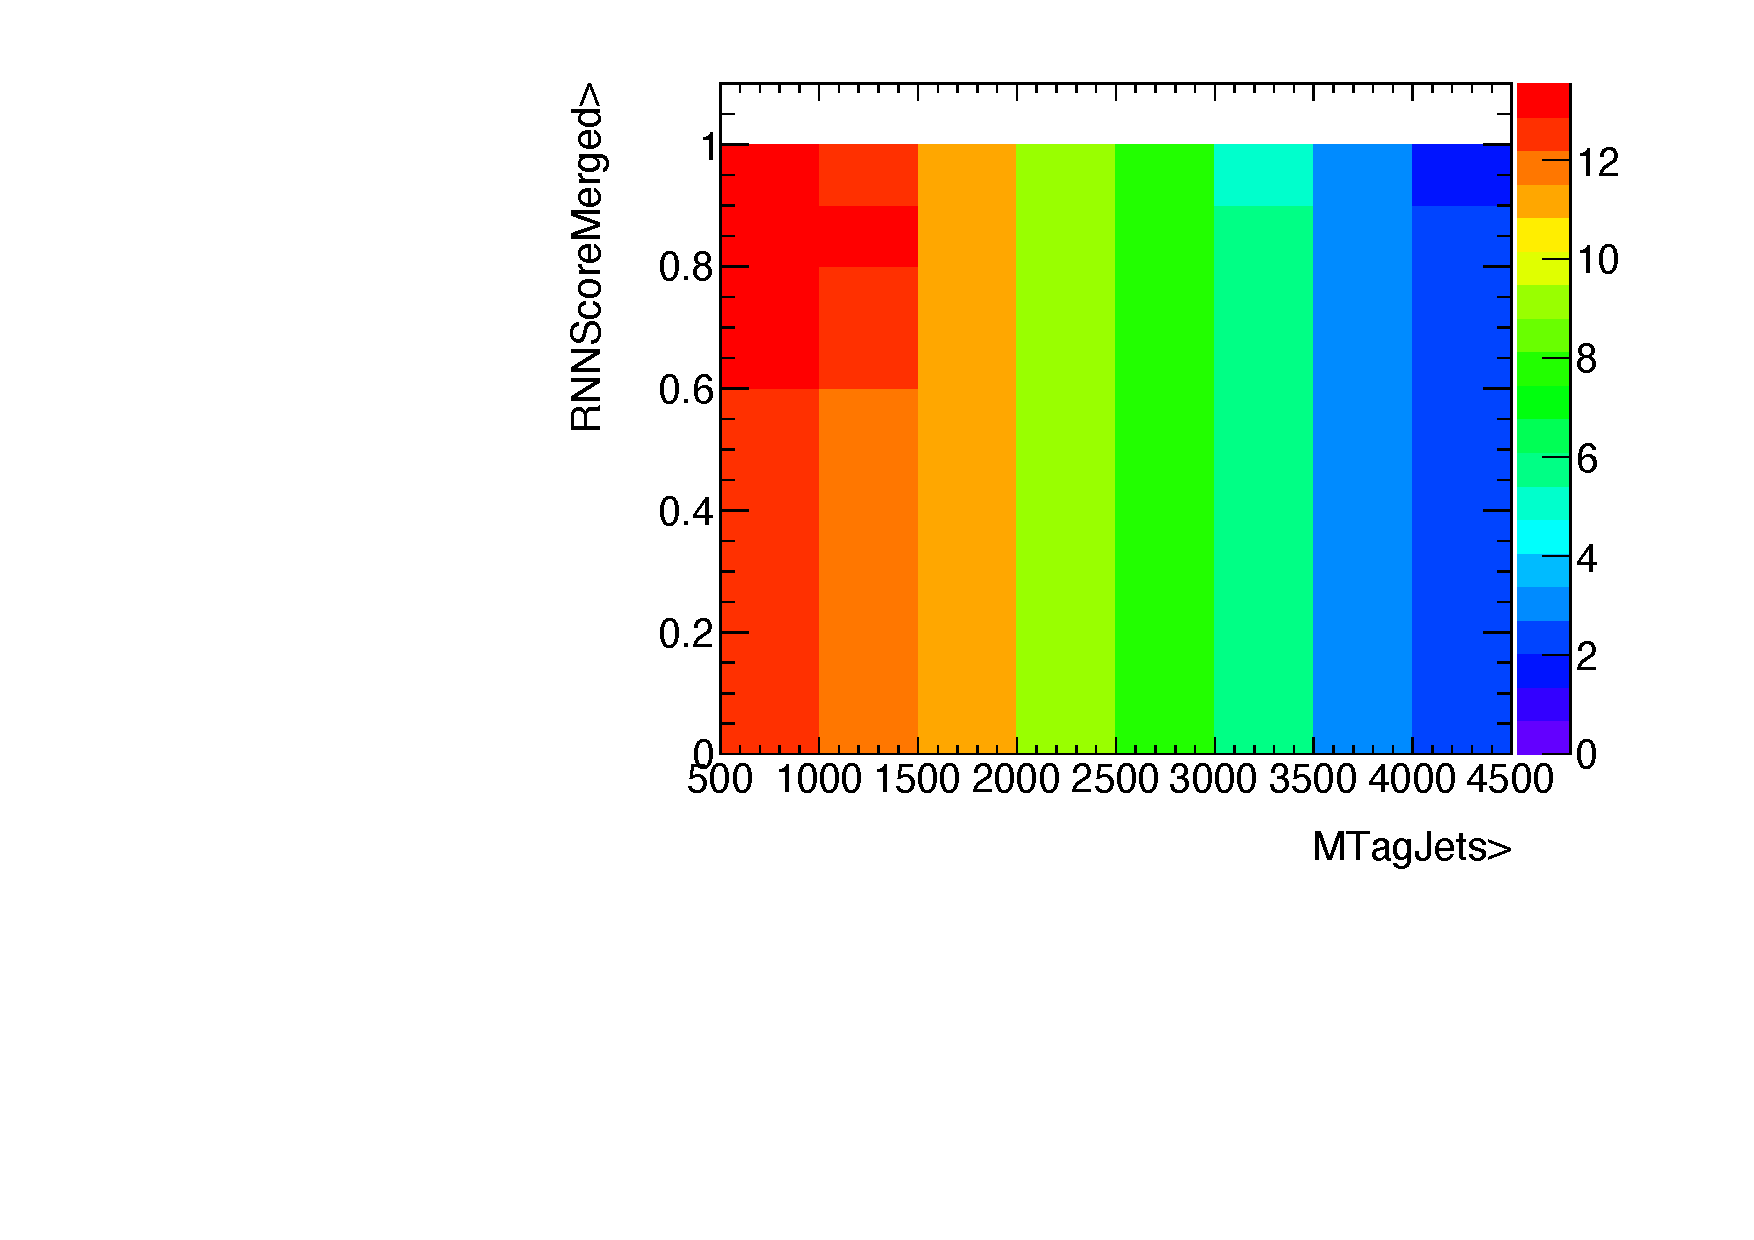
\includegraphics[width=0.30\textwidth]{figures/aQGC/HPSRFT0MVV.pdf}
    	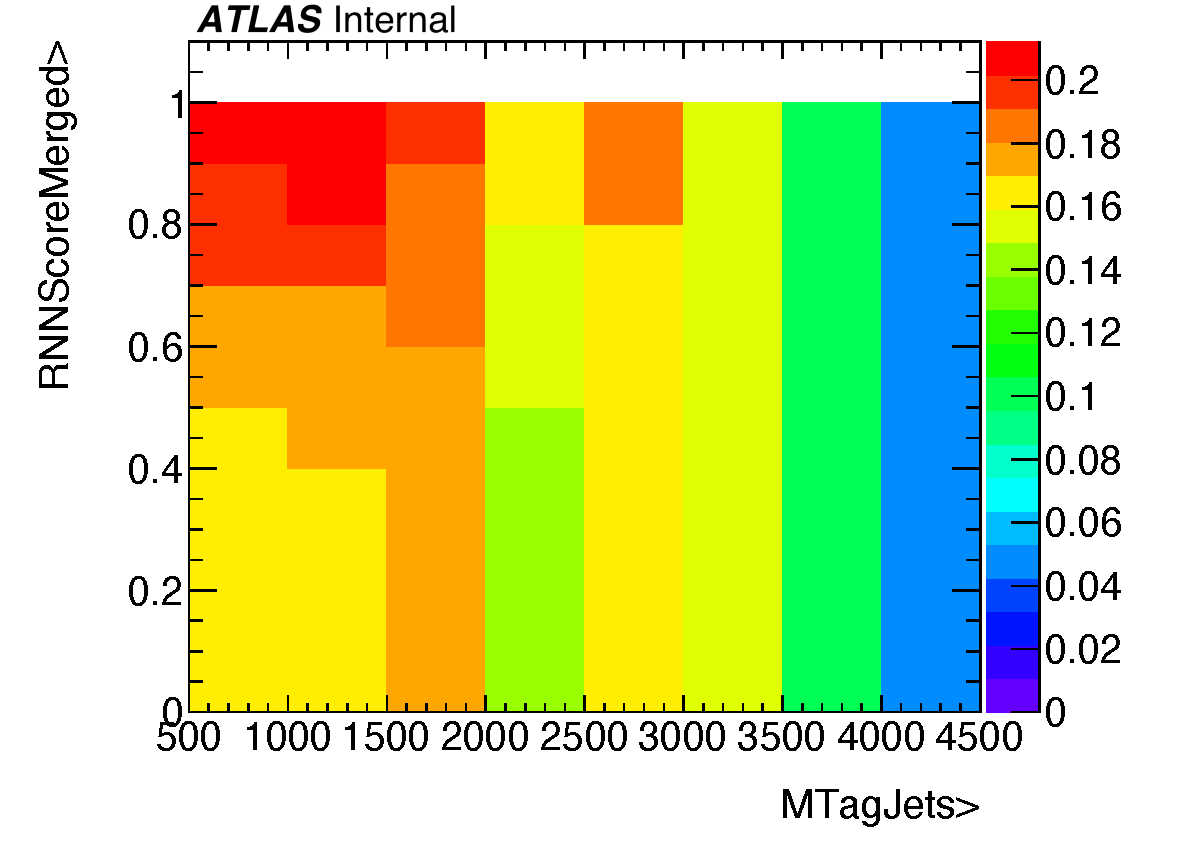
\includegraphics[width=0.30\textwidth]{figures/aQGC/HPSRFS02MVV.pdf}
    	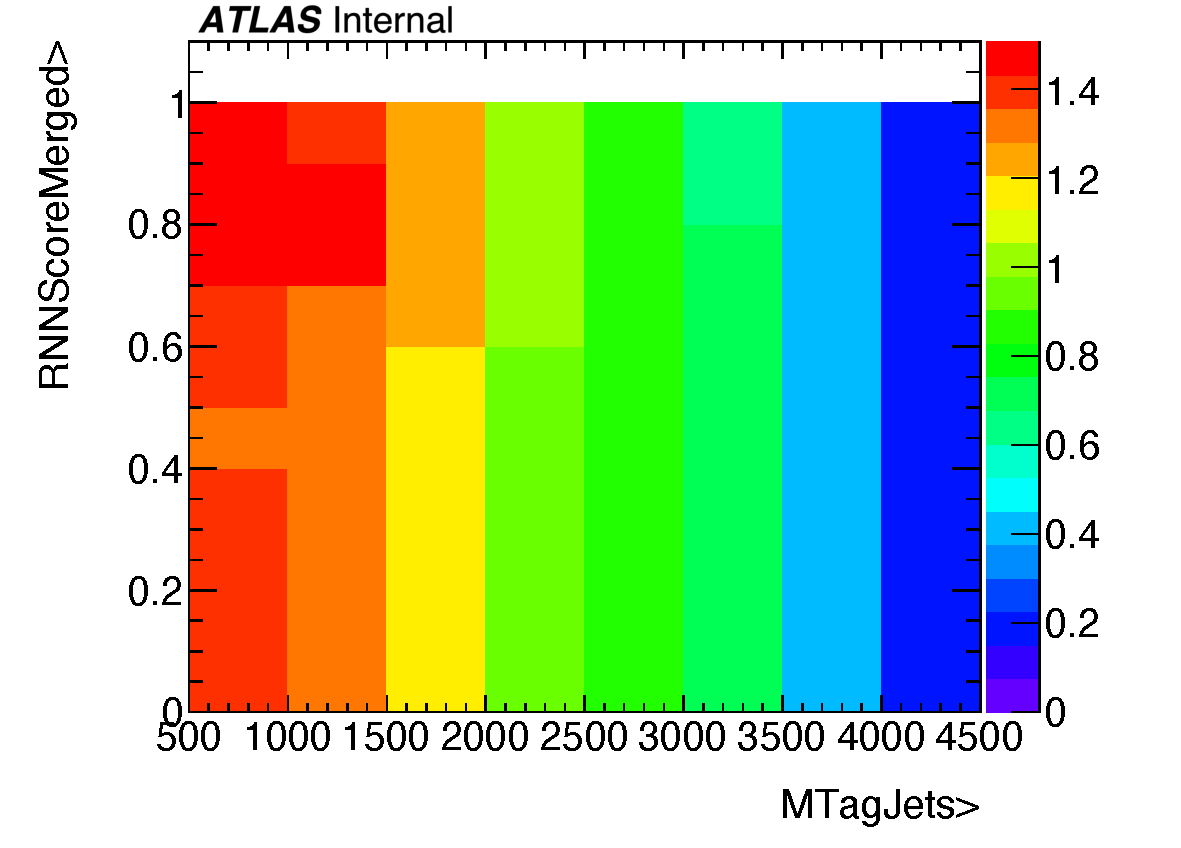
\includegraphics[width=0.30\textwidth]{figures/aQGC/HPSRFM0MVV.pdf}
        \caption{The 2D scan of the binned significance of operator FT0 (left), FS02 (middle), FM0 (right) with $m_{VV}$ score as discriminant in Merged HP signal region. Only quadratic terms are scanned.}
        \label{fig:2lepaQGCBinnedSigMVV}
\end{figure}

\begin{figure}[ht]
    \centering
    	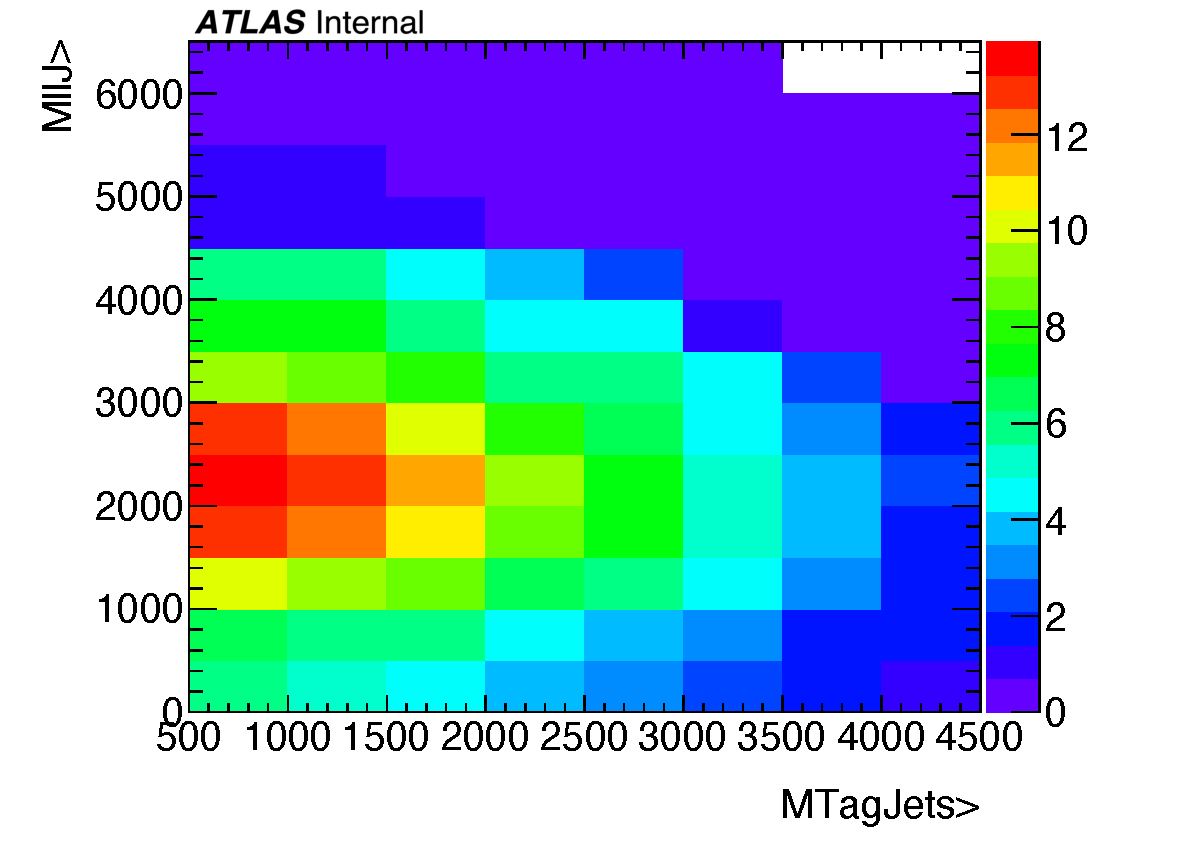
\includegraphics[width=0.30\textwidth]{figures/aQGC/HPSRFT0RNN.pdf}
    	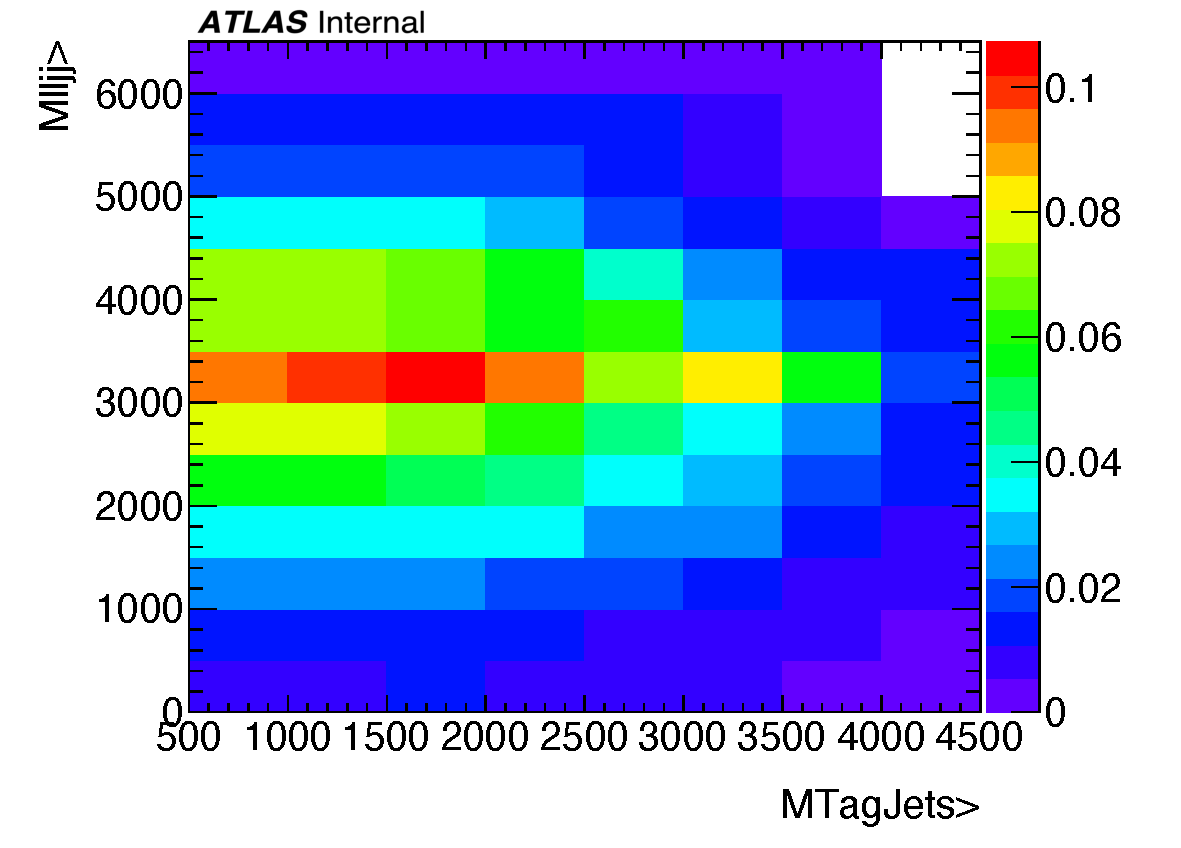
\includegraphics[width=0.30\textwidth]{figures/aQGC/HPSRFS02RNN.pdf}
    	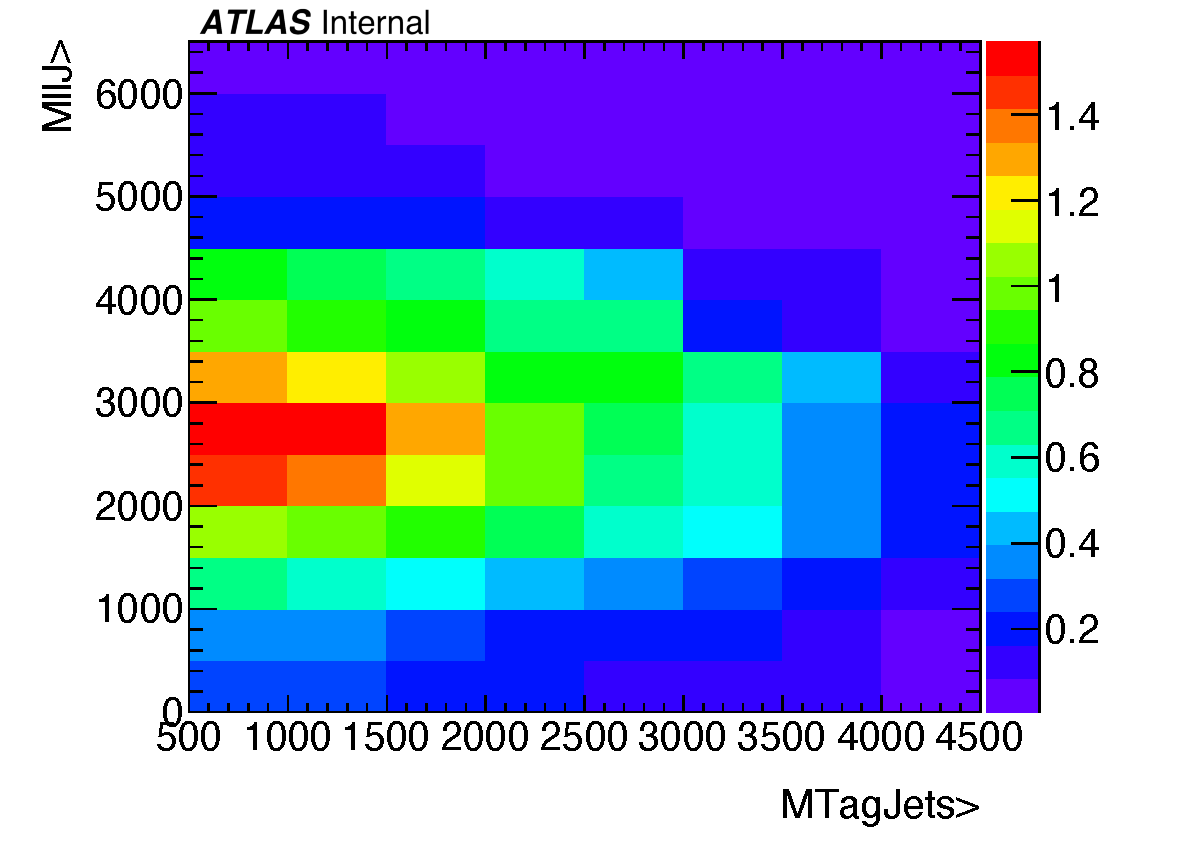
\includegraphics[width=0.30\textwidth]{figures/aQGC/HPSRFM0RNN.pdf}
        \caption{The 2D scan of the binned significance of operator FT0 (left), FS02 (middle), FM0 (right) with RNN score as discriminant in Merged HP signal region. Only quadratic terms are scanned.}
        \label{fig:2lepaQGCBinnedSigRNN}
\end{figure}

\clearpage

\begin{table}[ht!]
\small
\begin{center}
\resizebox{0.50\textwidth}{!}{

 \begin{tabular}{ r ||  r  r  r  r  |}
    & $\mathrm{M}_{tagjj}$ (GeV) & RNN score  & significance before cut& significance  \tabularnewline \hline
FT0 & 500                        & 0.6        & 12.55                  & 12.98         \tabularnewline \hline
FT1 & 500                        & 0.6        & 11.94                  & 12.50         \tabularnewline \hline
FS02& 1000                       & 0.8        & 0.17                   & 0.20          \tabularnewline \hline
FS1 & 500                        & 0.8        & 0.07                   & 0.07          \tabularnewline \hline
FM0 & 500                        & 0.7        & 1.36                   & 1.50          \tabularnewline \hline
FM1 & 500                        & 0.3        & 0.25                   & 0.27          \tabularnewline \hline
FM2 & 500                        & 0.7        & 0.82                   & 0.93          \tabularnewline \hline
FM3 & 500                        & 0.6        & 0.15                   & 0.16          \tabularnewline \hline
FM4 & 500                        & 0.7        & 0.38                   & 0.42          \tabularnewline \hline
FM5 & 500                        & 0.7        & 0.23                   & 0.25          \tabularnewline \hline
FM7 & 500                        & 0.6        & 0.12                   & 0.12          \tabularnewline \hline

\end{tabular}
}
\caption{Best cut point table for binned significance for $m_{VV}$ score distribution in \tlep channel in HPSR}
\label{tab:2lep_HPSR_MVV}
\end{center}
\end{table}

\begin{table}[ht!]
\small
\begin{center}
\resizebox{0.50\textwidth}{!}{

 \begin{tabular}{ r ||  r  r  r  r  |}
    & $\mathrm{M}_{tagjj}$ (GeV) & RNN score  & significance before cut & significance \tabularnewline \hline
FT0 & 500          & 0.1  & 6.65      & 6.77                          \tabularnewline \hline
FT1 & 500          & 0.2  & 6.69      & 6.85                          \tabularnewline \hline
FS02& 500          & 0.9  & 0.05      & 0.10                          \tabularnewline \hline
FS1 & 1000         & 0.8  & 0.02      & 0.04                          \tabularnewline \hline
FM0 & 500          & 0.8  & 0.54      & 0.12                          \tabularnewline \hline
FM1 & 500          & 0.1  & 0.08      & 0.42                          \tabularnewline \hline
FM2 & 500          & 0.9  & 0.28      & 0.08                          \tabularnewline \hline
FM3 & 1000         & 0.8  & 0.05      & 0.18                          \tabularnewline \hline
FM4 & 1000         & 0.8  & 0.12      & 0.10                          \tabularnewline \hline
FM5 & 1000         & 0.8  & 0.07      & 0.10                          \tabularnewline \hline
FM7 & 500          & 0.1  & 0.04      & 0.06                          \tabularnewline \hline

\end{tabular}
}
\caption{Best cut point table for binned significance for $m_{VV}$ score distribution in \tlep channel in LPSR}
\label{tab:2lep_LPSR_MVV}
\end{center}
\end{table}

\begin{table}[ht!]
\small
\begin{center}
\resizebox{0.50\textwidth}{!}{

 \begin{tabular}{ r ||  r  r  r  r  |}
    & $\mathrm{M}_{tagjj}$ (GeV) & MllJ (GeV) & significance before cut& significance \tabularnewline \hline
FT0 & 500          & 2000   & 5.62    & 13.92                           \tabularnewline \hline
FT1 & 500          & 2000   & 5.25    & 13.31                           \tabularnewline \hline
FS02& 1500         & 3000   & 0.01    & 0.11                            \tabularnewline \hline
FS1 & 2500         & 3000   & 0.01    & 0.07                            \tabularnewline \hline
FM0 & 500          & 2500   & 0.27    & 1.57                            \tabularnewline \hline
FM1 & 500          & 2500   & 0.03    & 0.28                            \tabularnewline \hline
FM2 & 500          & 2500   & 0.14    & 0.95                            \tabularnewline \hline
FM3 & 500          & 3000   & 0.01    & 0.12                            \tabularnewline \hline
FM4 & 500          & 2500   & 0.06    & 0.45                            \tabularnewline \hline
FM5 & 500          & 2500   & 0.03    & 0.25                            \tabularnewline \hline
FM7 & 500          & 2500   & 0.01    & 0.12                            \tabularnewline \hline

\end{tabular}
}
\caption{Best cut point table for binned significance for RNN score distribution in \tlep channel in HPSR}
\label{tab:2lep_HPSR_RNN}
\end{center}
\end{table}

\begin{table}[ht!]
\small
\begin{center}
\resizebox{0.50\textwidth}{!}{

 \begin{tabular}{ r ||  r  r  r  r  |}
    & $\mathrm{M}_{tagjj}$ (GeV) & MllJ (GeV) & significance before cut& significance \tabularnewline \hline
FT0 & 500          & 2000  & 2.64     & 7.72                            \tabularnewline \hline
FT1 & 500          & 2000  & 2.80     & 7.46                            \tabularnewline \hline
FS02& 1500         & 3000  & 0.01     & 0.06                            \tabularnewline \hline
FS1 & 500          & 3000  & 0.00     & 0.06                            \tabularnewline \hline
FM0 & 500          & 2500  & 0.12     & 0.92                            \tabularnewline \hline
FM1 & 500          & 3000  & 0.02     & 0.18                            \tabularnewline \hline
FM2 & 500          & 3000  & 0.06     & 0.54                            \tabularnewline \hline
FM3 & 500          & 3000  & 0.01     & 0.12                            \tabularnewline \hline
FM4 & 500          & 3000  & 0.03     & 0.26                            \tabularnewline \hline
FM5 & 500          & 3000  & 0.01     & 0.16                            \tabularnewline \hline
FM7 & 500          & 3000  & 0.01     & 0.09                            \tabularnewline \hline

\end{tabular}
}
\caption{Best cut point table for binned significance for RNN score distribution in \tlep channel LPSR}
\label{tab:2lep_LPSR_RNN}
\end{center}
\end{table}

Comparing the significance between table~\ref{tab:2lep_HPSR_MVV} and table~\ref{tab:2lep_HPSR_RNN}, 
RNN score as discriminant with $m_{VV}$ cut around 2.5~TeV shows slightly better but not so different ability with the $m_{VV}$ without any cut.
It seems to be the simple and better way to use $m_{VV}$ as the discriminant without cut. 

Following the study of this section, the profile likelihood fit with $m_{VV}$ score is performed and the expected limit is shown in section~\ref{subsec:aqgc_limit}. The fit study with RNN score as discriminant is also shown in section~\ref{subsec:2binapproach}.

%\section{Expected limit}
%\label{subsec:aqgc_limit}

%The expected upper limit on each Wilson coefficient by a combined fit of all 3 channels is shown in table~\ref{tab:aQGC_limit}, which is calculated by $\sqrt{\mu_{95\%}} = f_{i} / \Lambda^4$, where $\mu_{95\%}$ is the 95\% upper limit on the signal strength.
%The $m_{VV}$ distributions without any additional cuts are used in the fit.
%The systematic uncertainties are yet to be included.
%Figures~\ref{fig:0lepFT0} and ~\ref{fig:1lepFT0}, ~\ref{fig:2lepFT0} show the prefit plots of %$m_{VV}$ distribution. FT0 signal is overlaid.

%\begin{table}[ht!]
%\small
%\begin{center}
%\resizebox{0.30\textwidth}{!}{
% \begin{tabular}{ | r || r |}
%    & Expected limit (TeV$^{-4})$ \tabularnewline \hline
%FT0 & 0.14                        \tabularnewline \hline
%FT1 & 0.14                        \tabularnewline \hline
%FS02& 2.90                        \tabularnewline \hline
%FS1 & 4.56e+6                     \tabularnewline \hline
%FM0 & 0.85                        \tabularnewline \hline
%FM1 & 2.55                        \tabularnewline \hline
%FM2 & 1.26                        \tabularnewline \hline
%FM3 & 4.69e+2                     \tabularnewline \hline
%FM4 & 2.07                        \tabularnewline \hline
%FM5 & 81.3                        \tabularnewline \hline
%FM7 & 5.37e+2                     \tabularnewline \hline
%\end{tabular}
%}
%\caption{Expected upper limits of each Wilson coefficient. All 3 channels are combined.}
%\label{tab:aQGC_limit}
%\end{center}
%\end{table}

\begin{figure}[ht]
    \centering
    	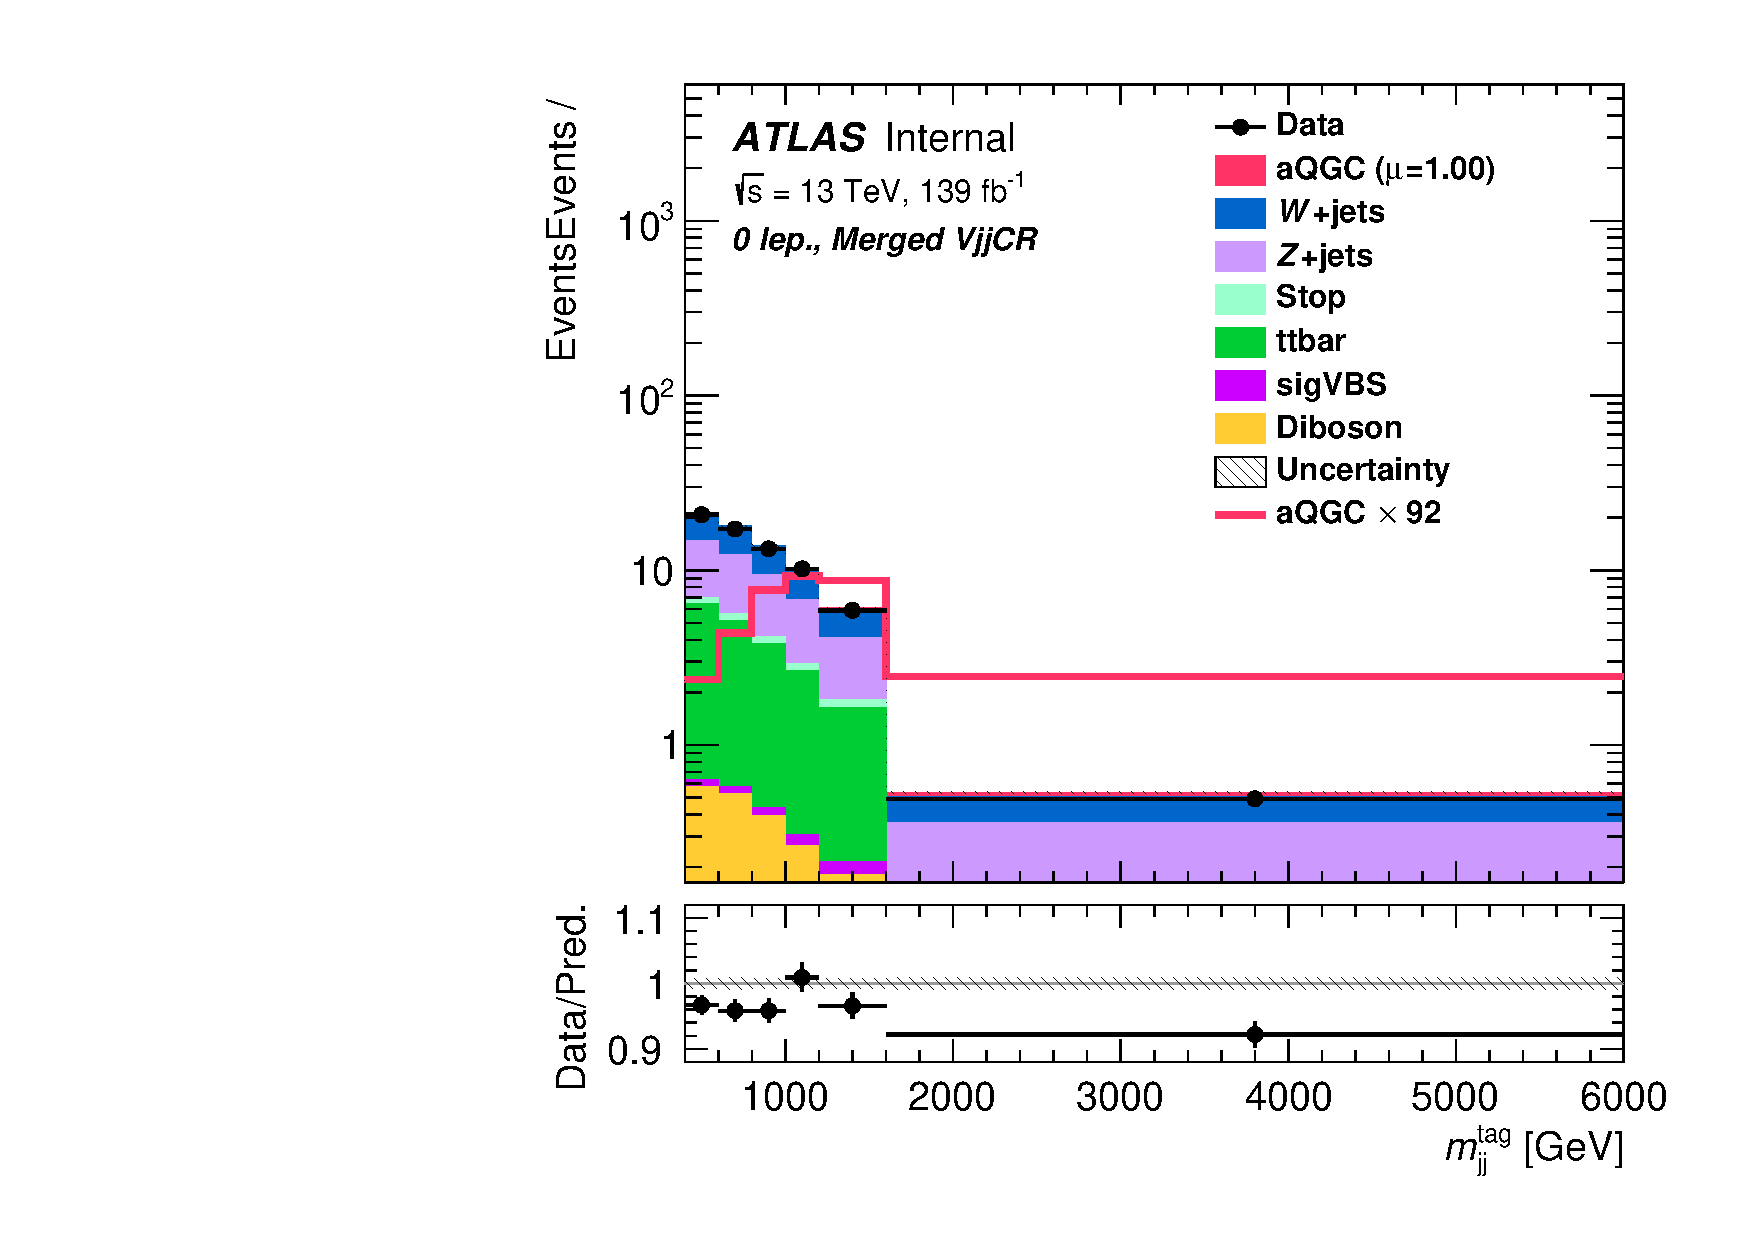
\includegraphics[width=0.35\textwidth]{figures/aQGC/Region_distMTagJets_DCRVjetMer_BMin0_J0_incJet1_L0_T0_incFat1_Y6051_incTag1_Fat1_Prefitlog.pdf}
    	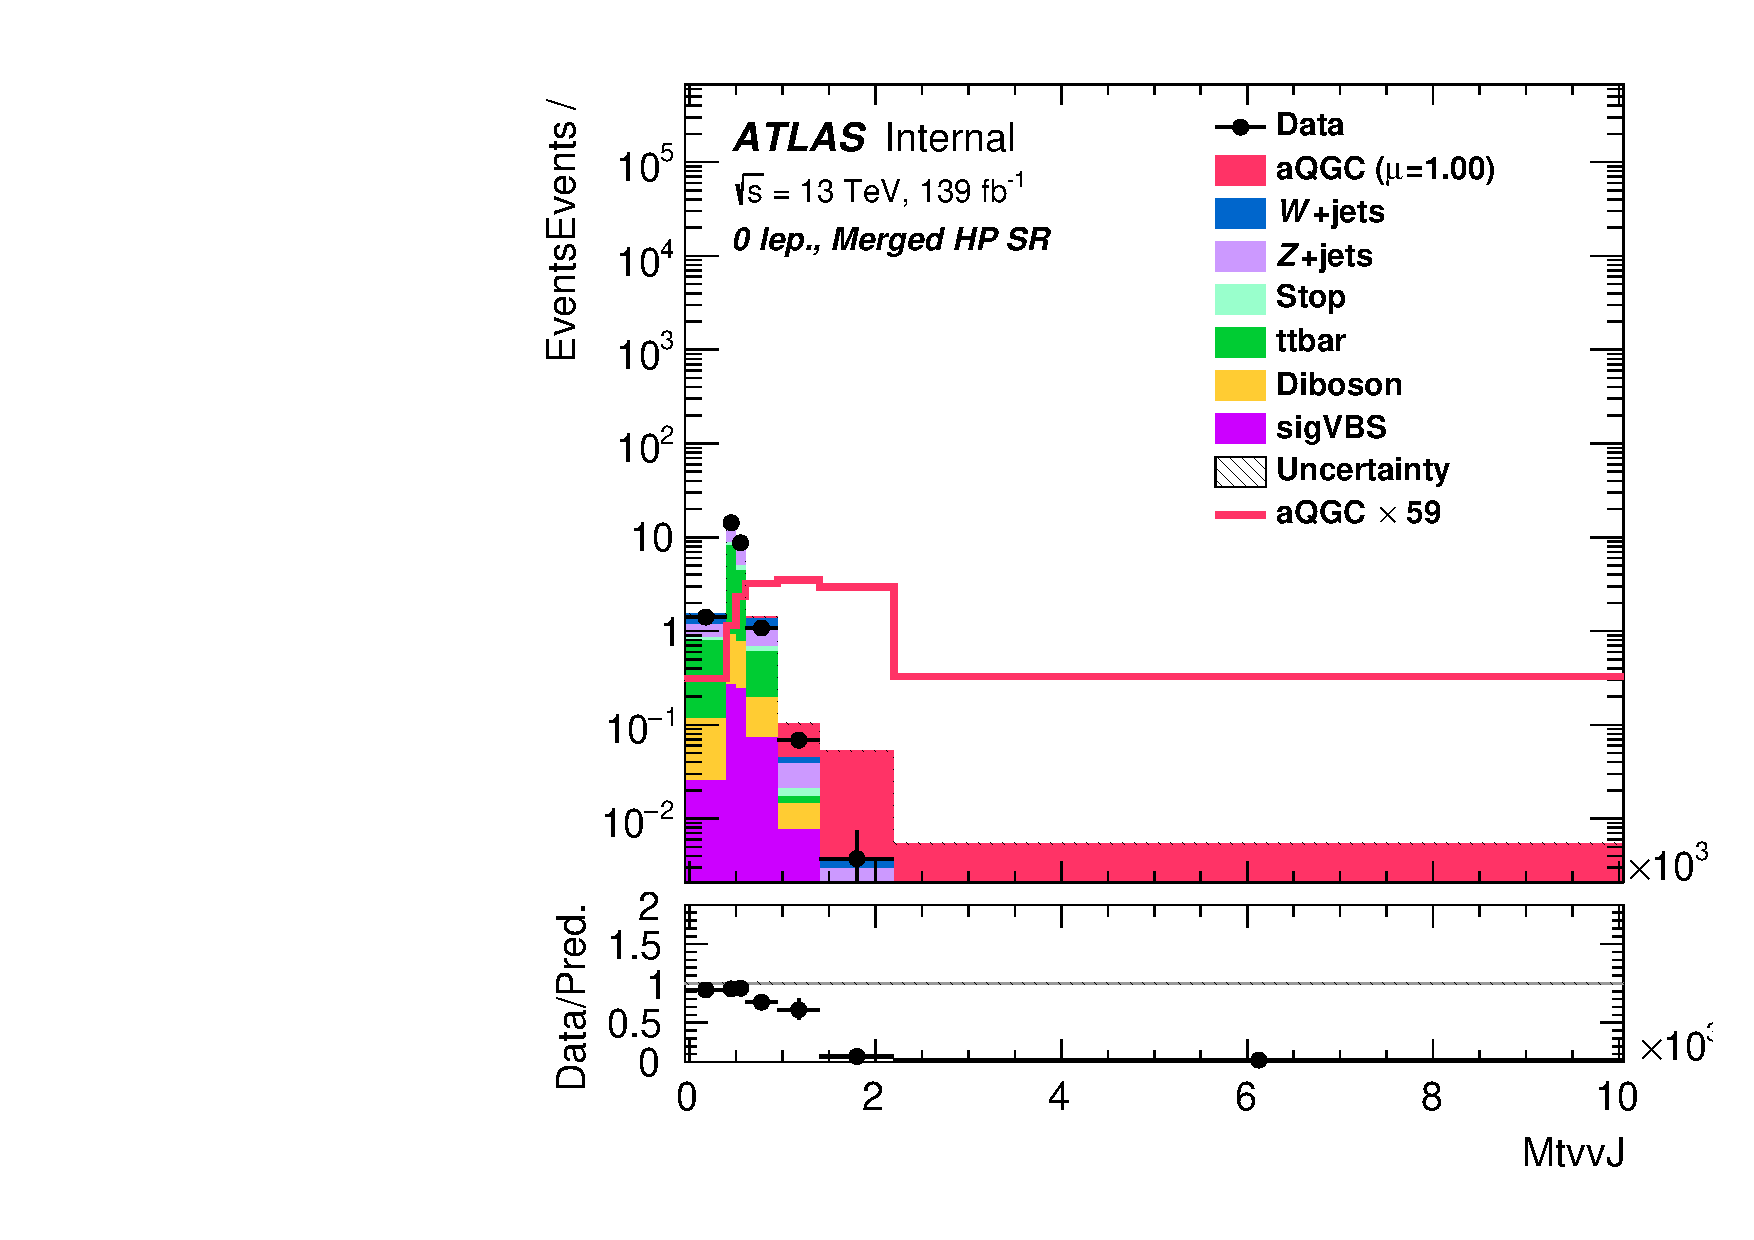
\includegraphics[width=0.35\textwidth]{figures/aQGC/Region_distMtvvJ_DSRVBSHP_BMin0_J0_incJet1_L0_T0_incFat1_Y6051_incTag1_Fat1_Prefitlog.pdf}
    	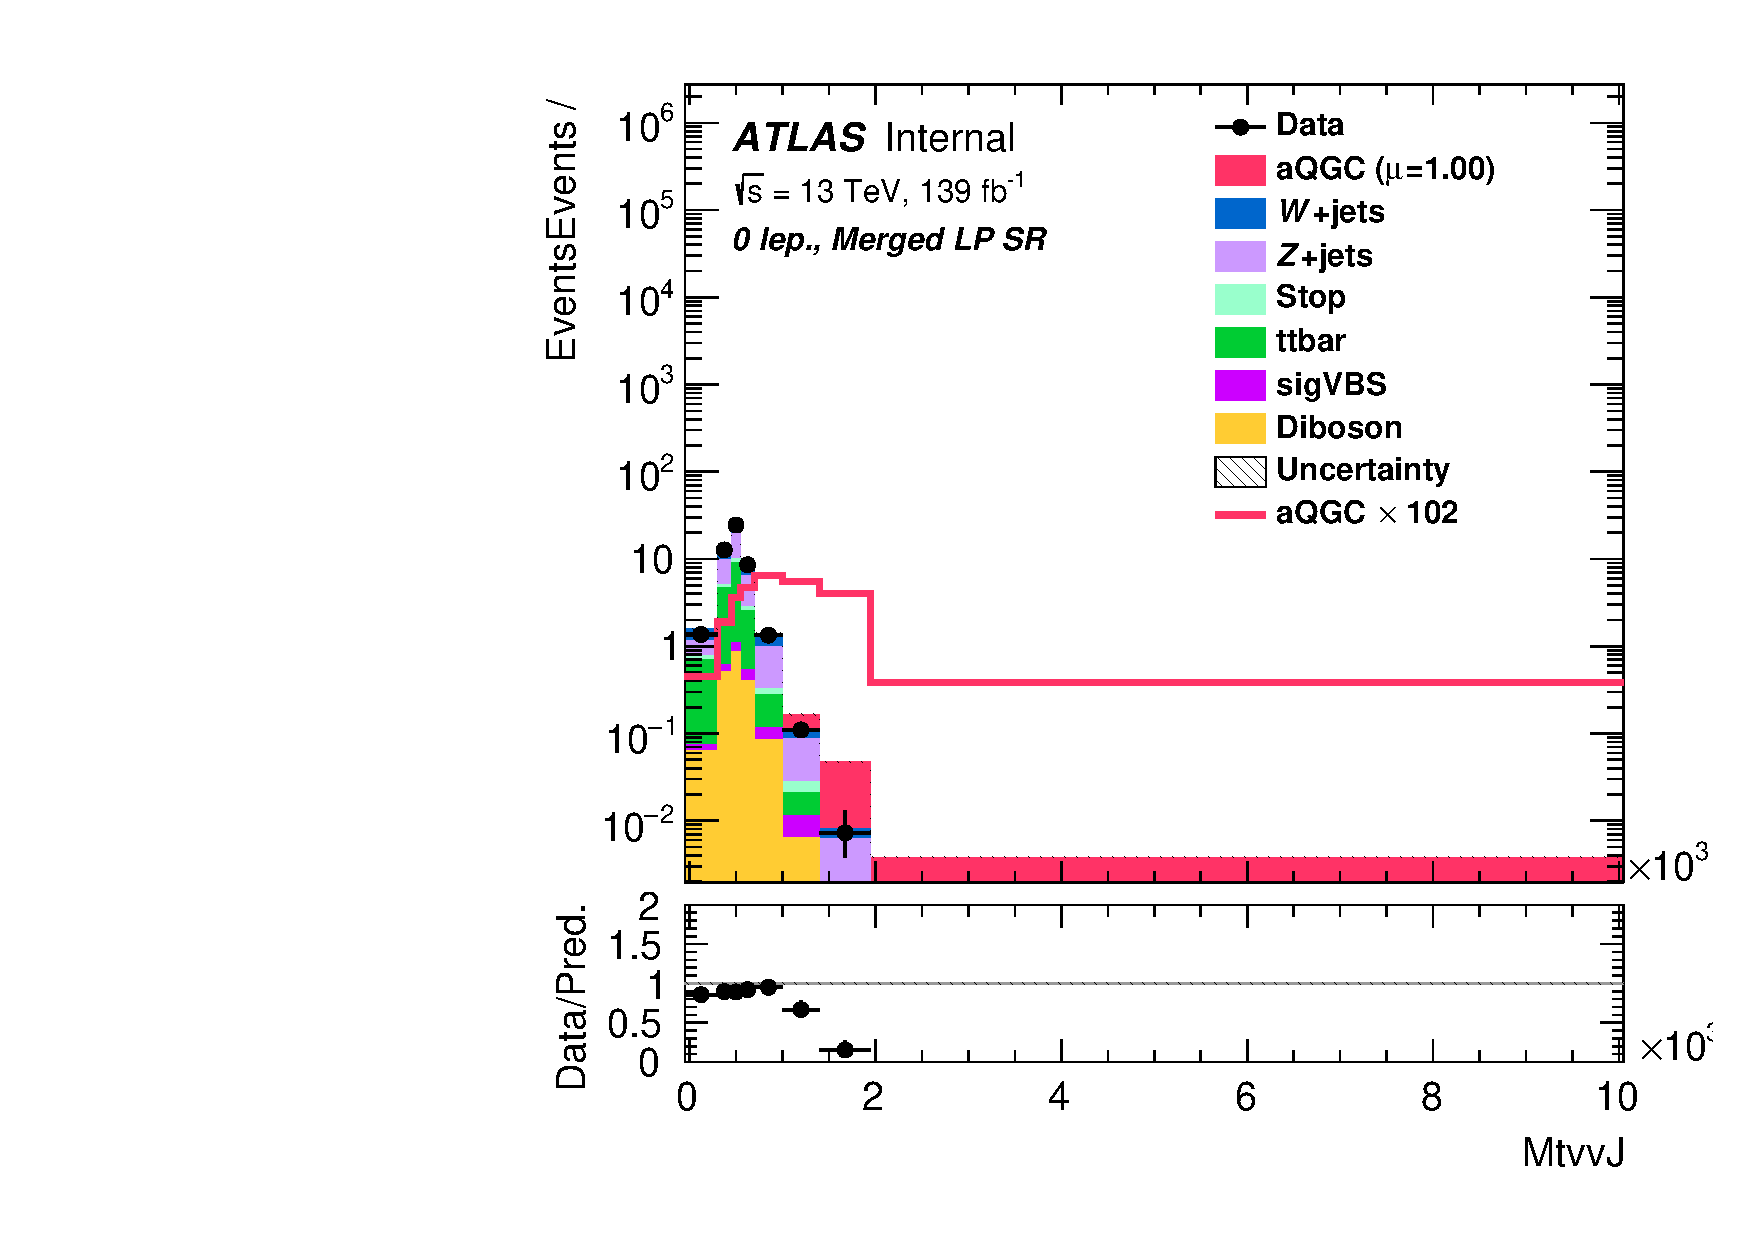
\includegraphics[width=0.35\textwidth]{figures/aQGC/Region_distMtvvJ_DSRVBSLP_BMin0_J0_incJet1_L0_T0_incFat1_Y6051_incTag1_Fat1_Prefitlog.pdf}
    	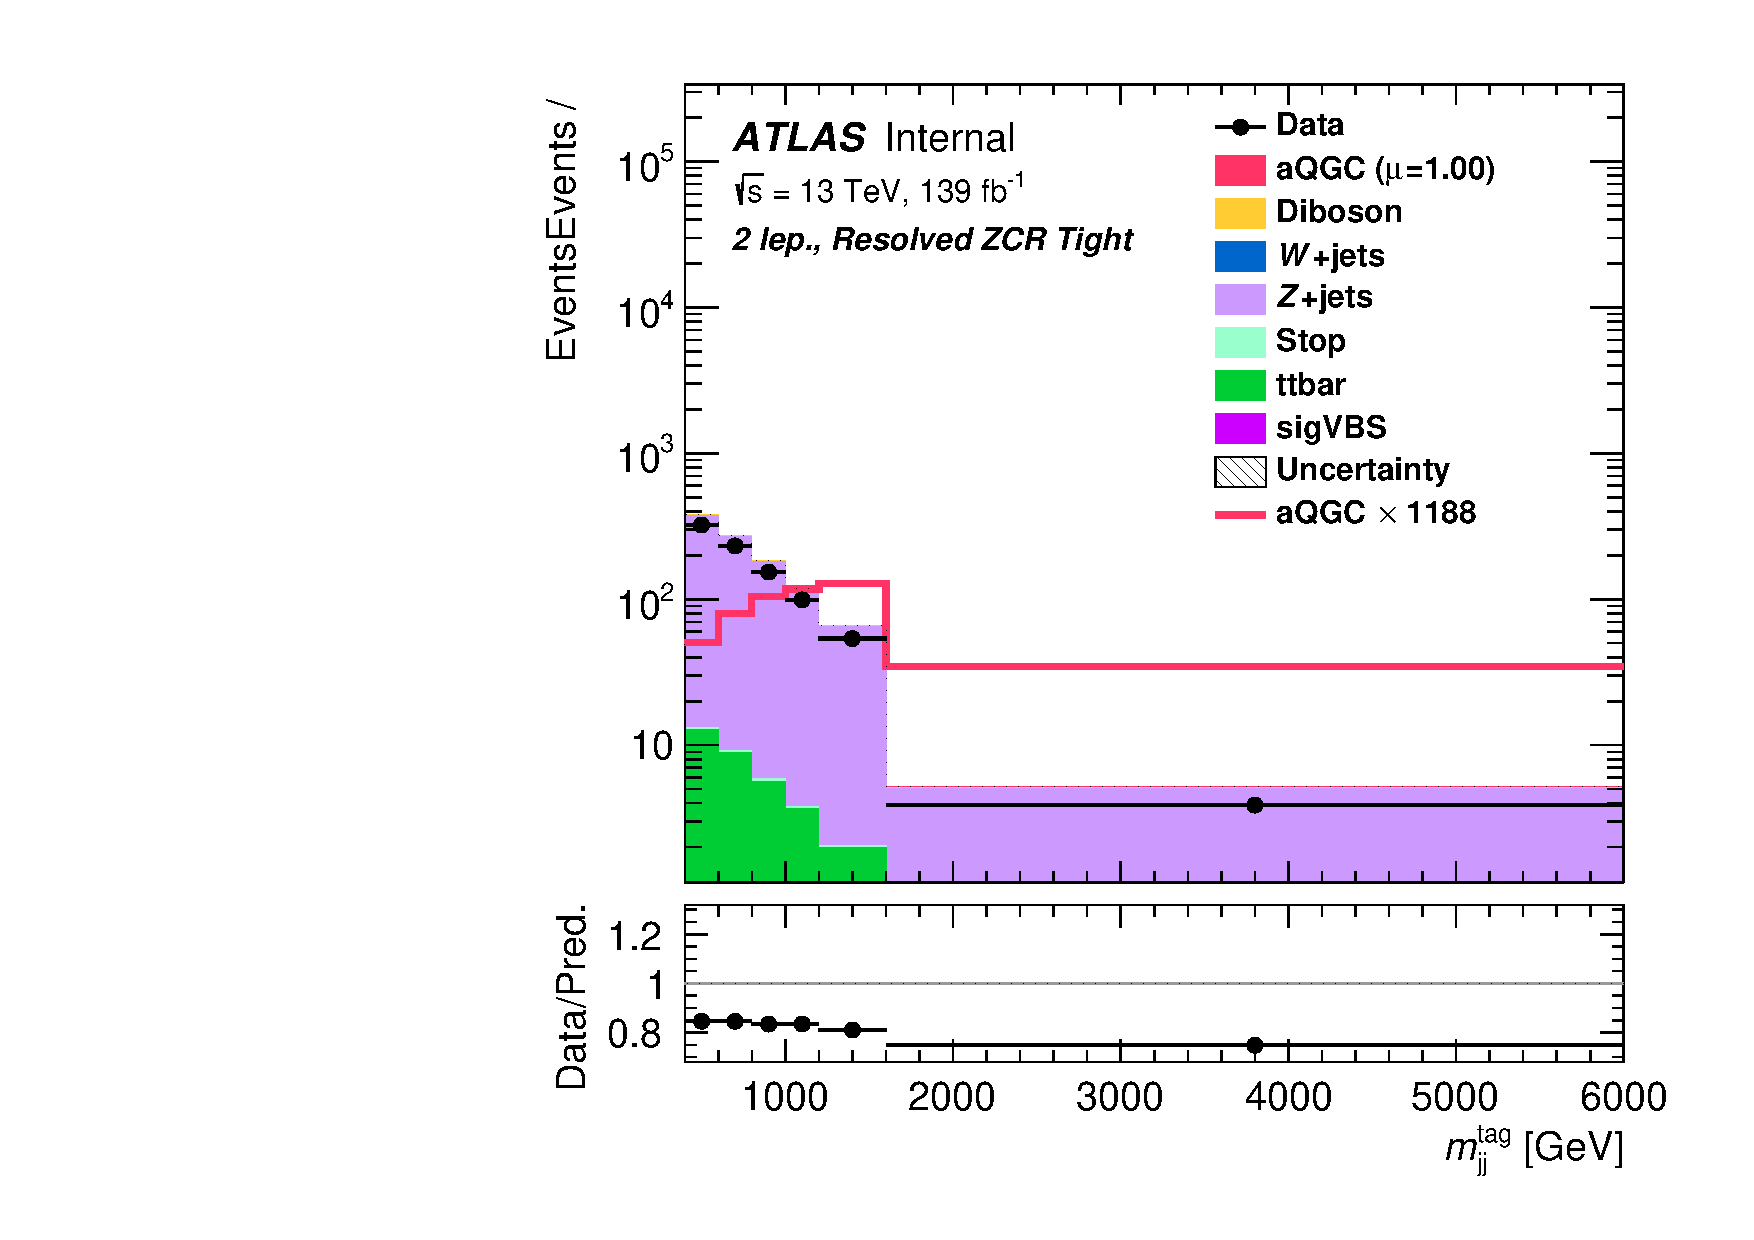
\includegraphics[width=0.35\textwidth]{figures/aQGC/Region_distMTagResJets_DCRVjetFid_BMin0_T0_Y6051_incTag1_J2_L2_incJet1_Prefitlog.pdf}
    	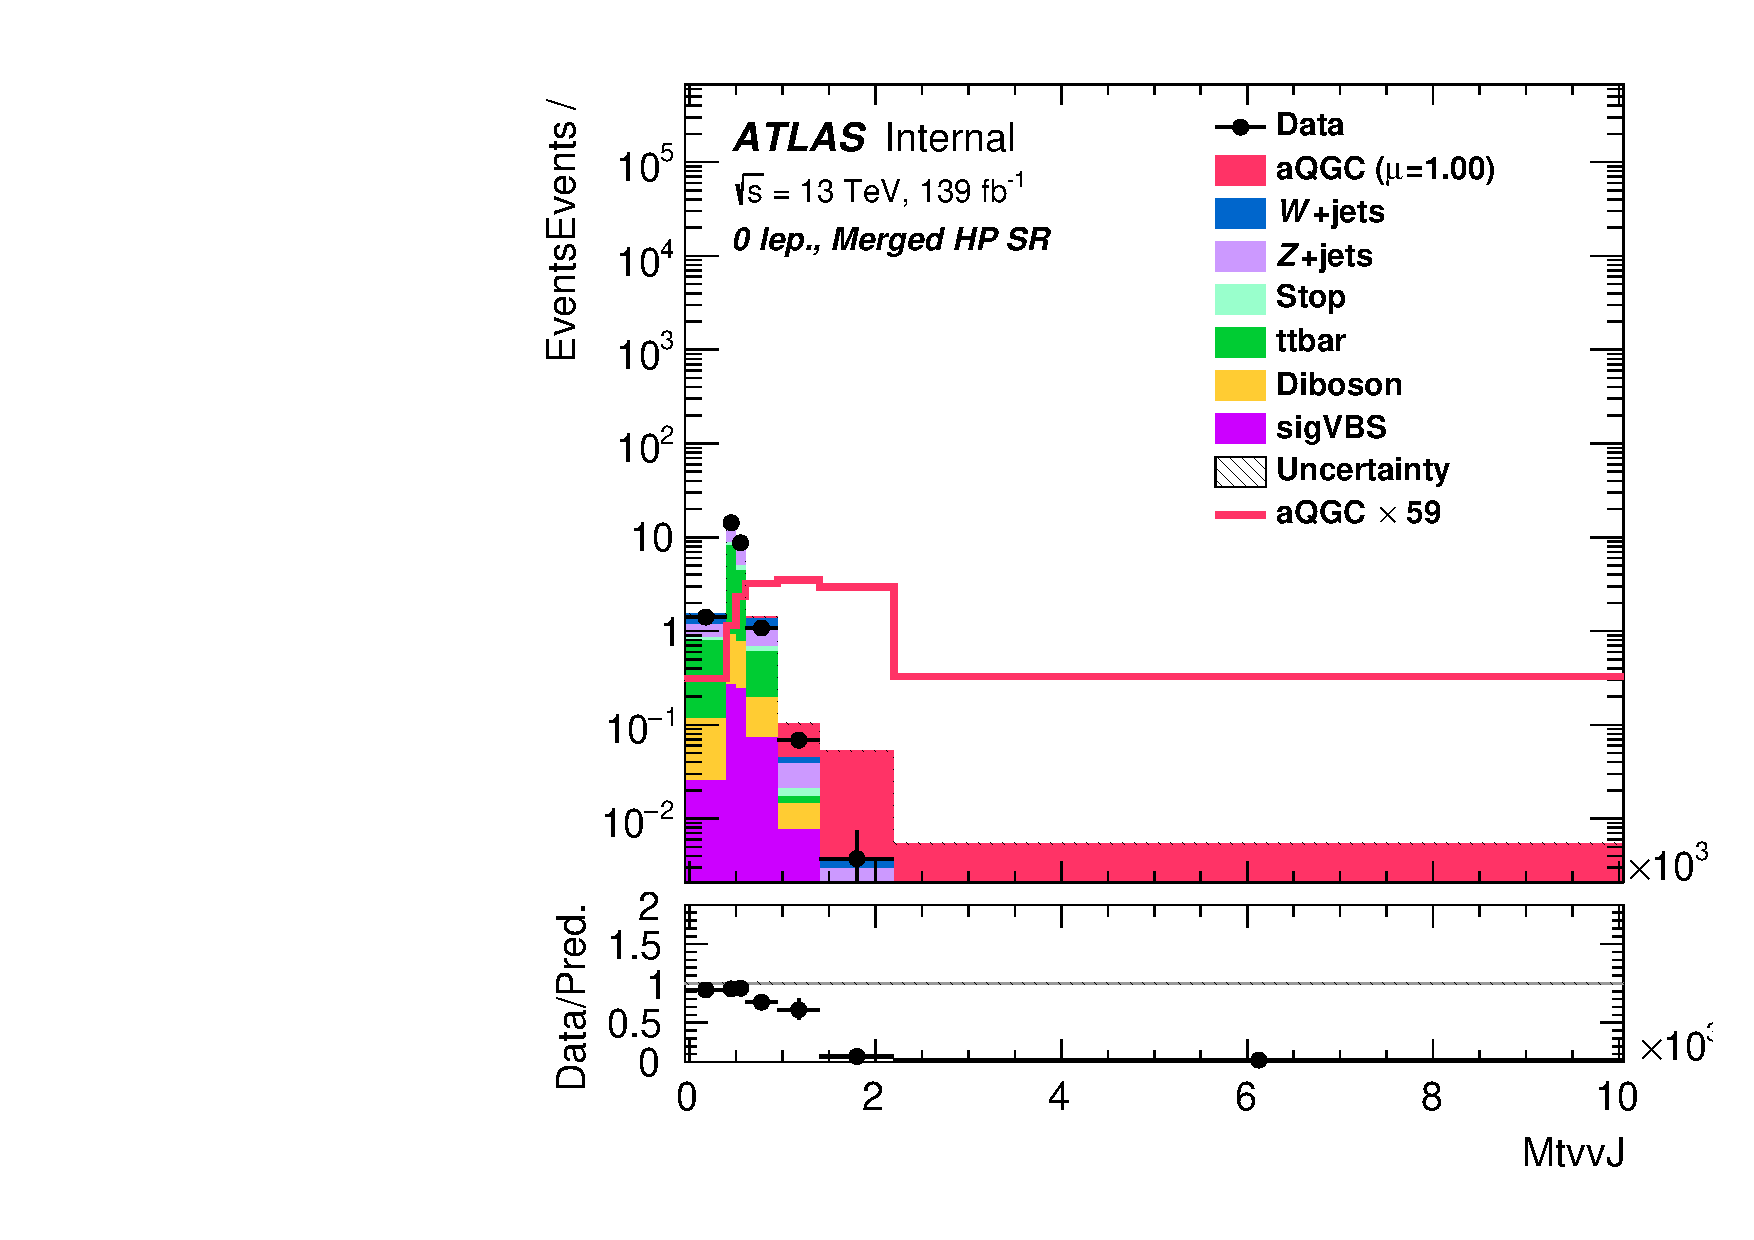
\includegraphics[width=0.35\textwidth]{figures/aQGC/Region_distMtvvJ_DSRVBSHP_BMin0_J0_incJet1_L0_T0_incFat1_Y6051_incTag1_Fat1_Prefitlog.pdf}
        \caption{Prefit plots for operator FT0 in \zlep channel are shown. The standard model EW signal is floated as the background.}
        \label{fig:0lepFT0}
\end{figure}

\begin{figure}[ht]
    \centering
    	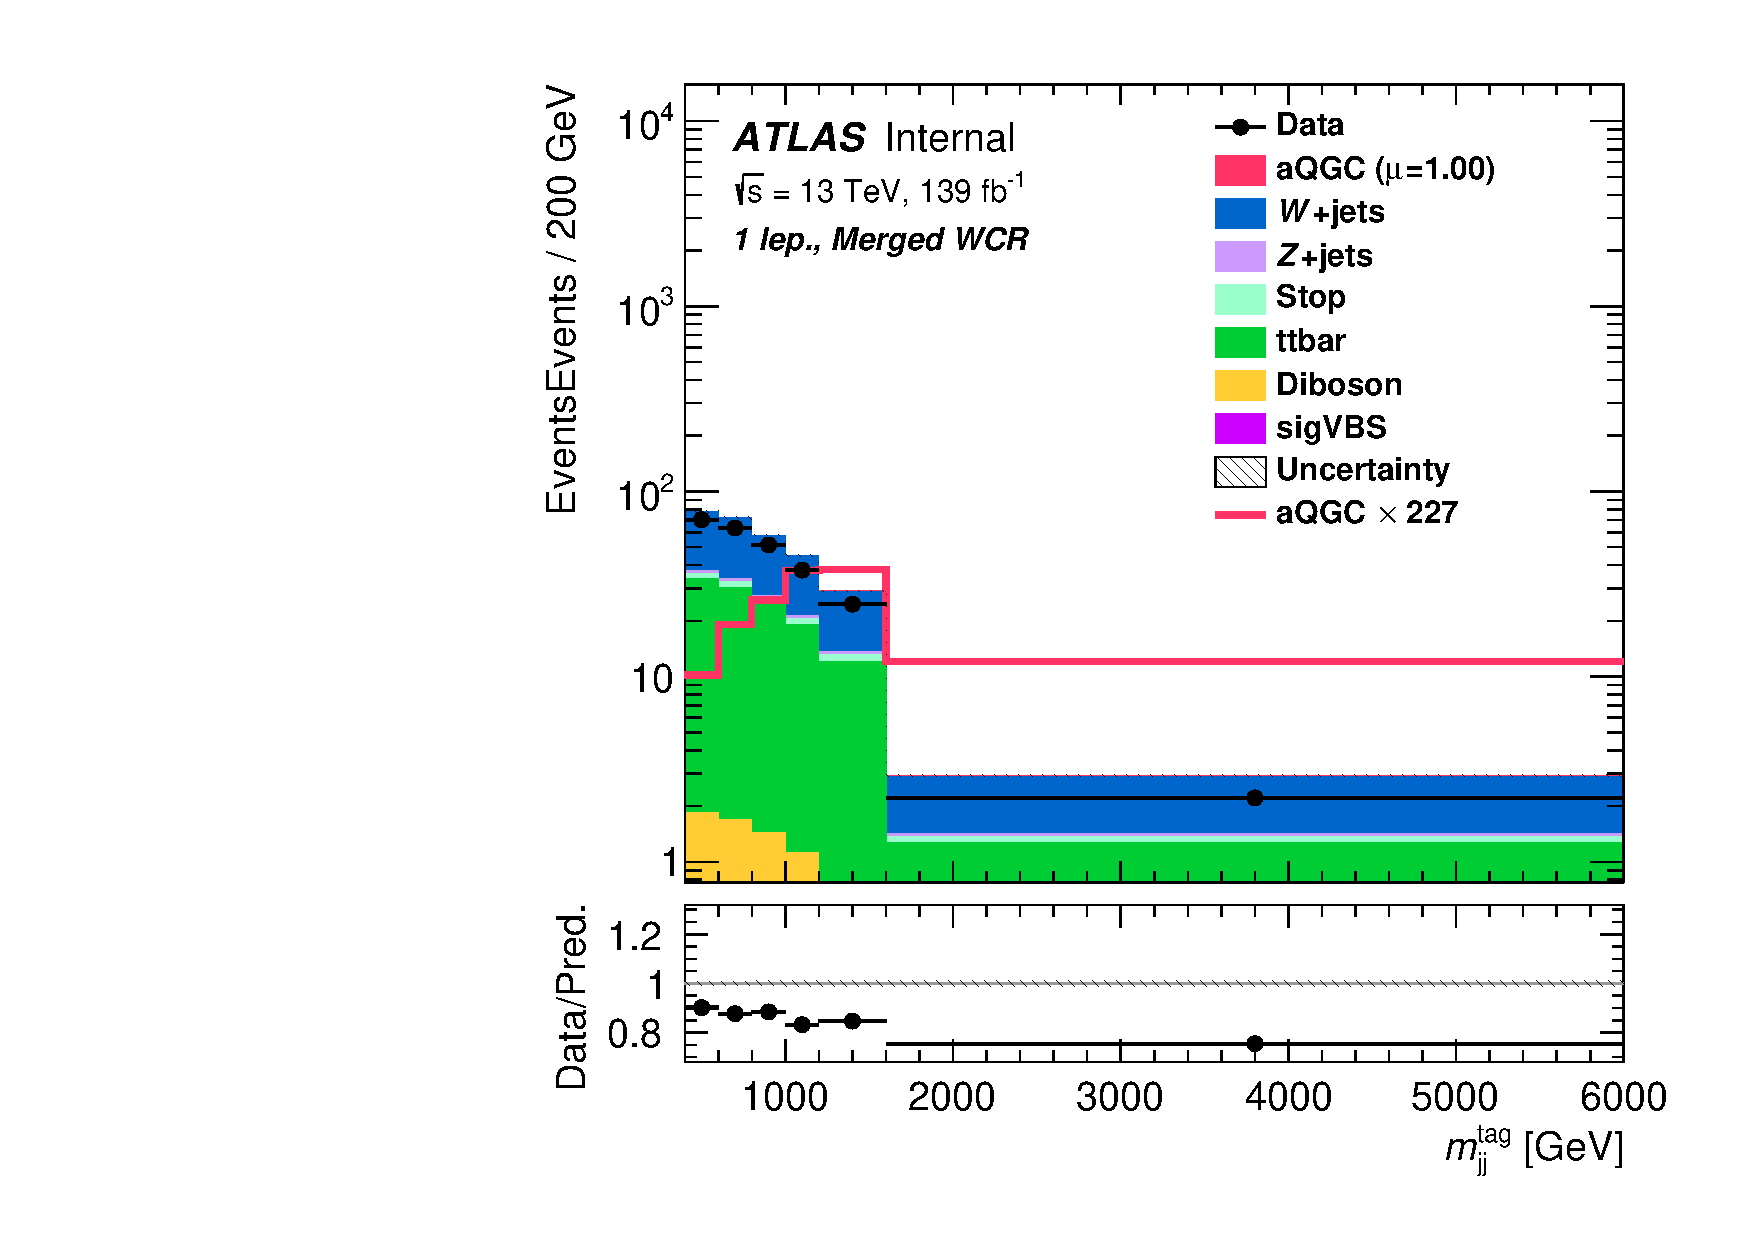
\includegraphics[width=0.35\textwidth]{figures/aQGC/Region_disttagMjj_DCRVjetMerged_BMin0_J0_incJet1_L1_T0_incFat1_Y6051_incTag1_Fat1_Prefitlog.pdf}
    	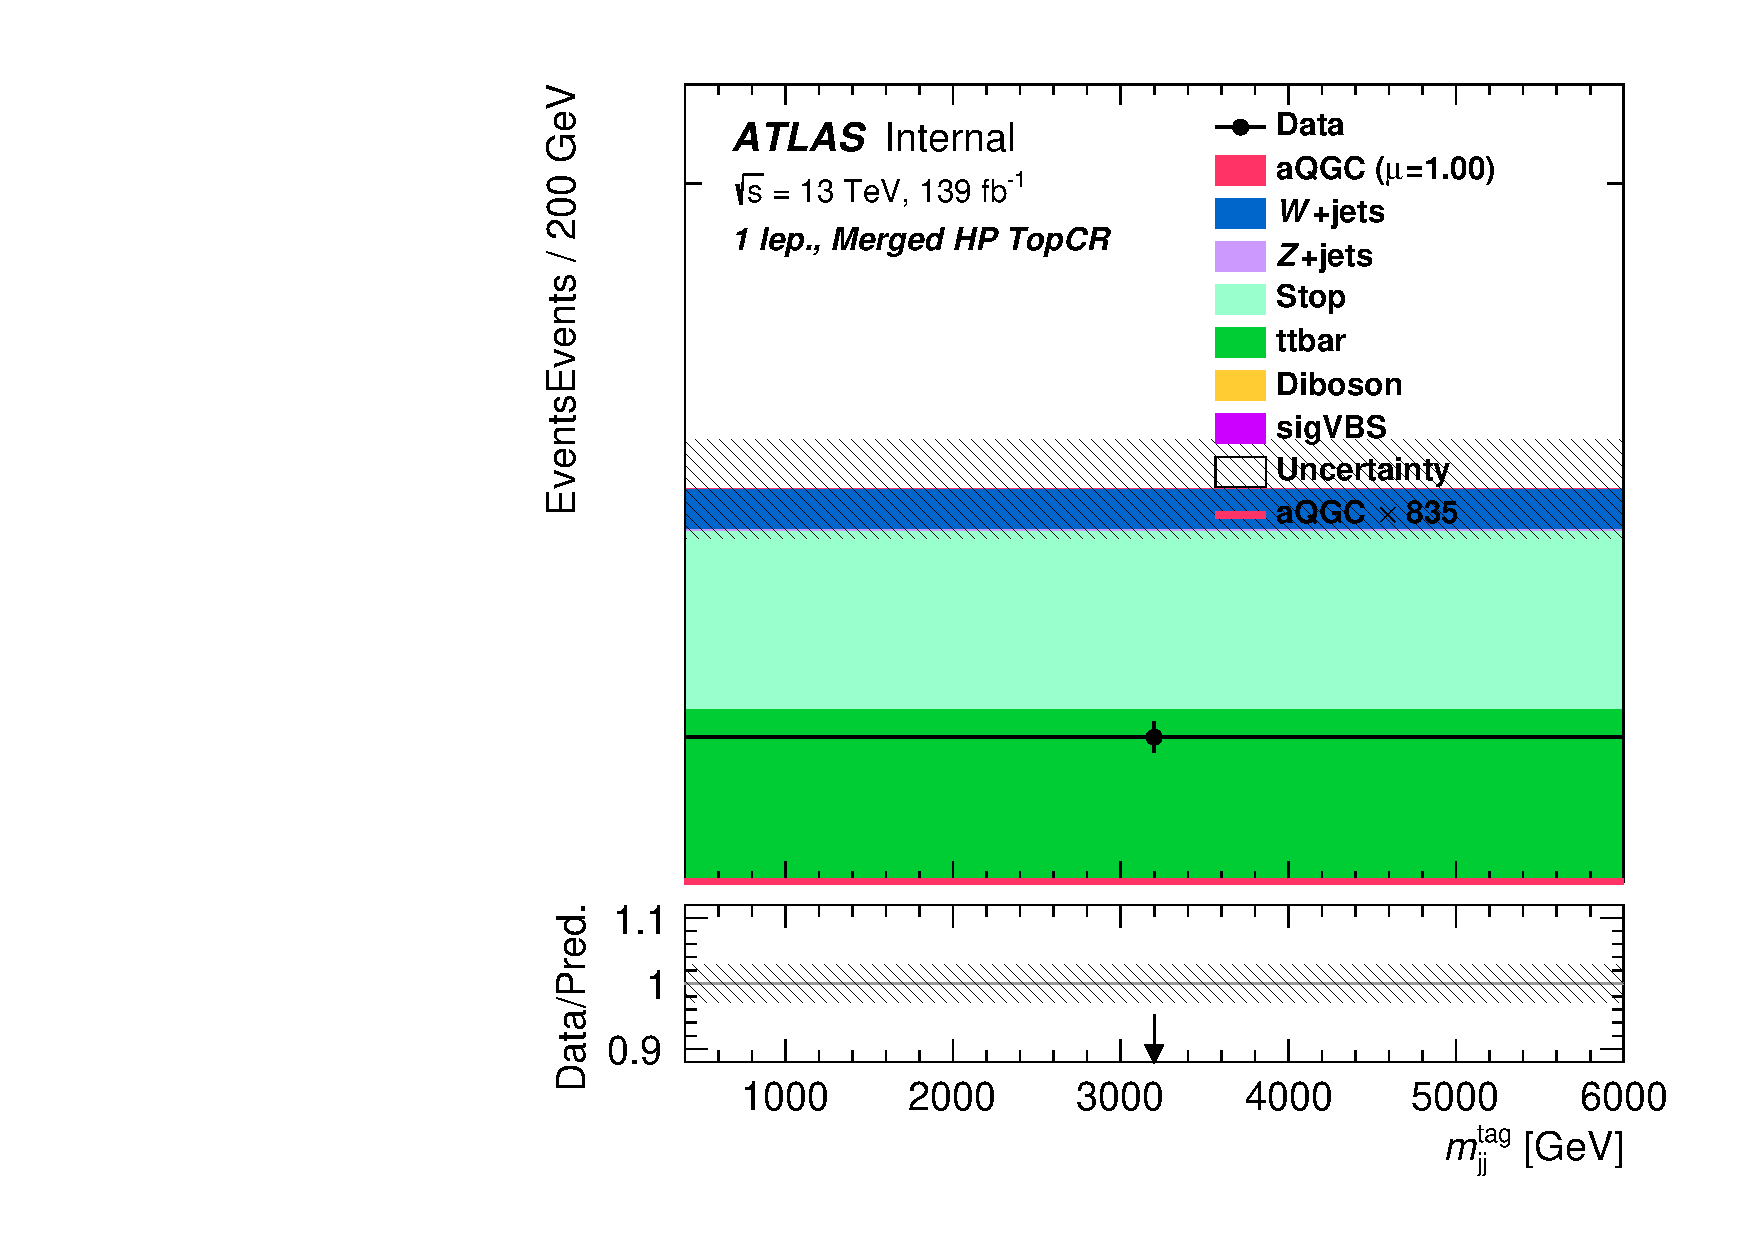
\includegraphics[width=0.35\textwidth]{figures/aQGC/Region_disttagMjj_DCRTopHP_BMin0_J0_incJet1_L1_T0_incFat1_Y6051_incTag1_Fat1_Prefitlog.pdf}
    	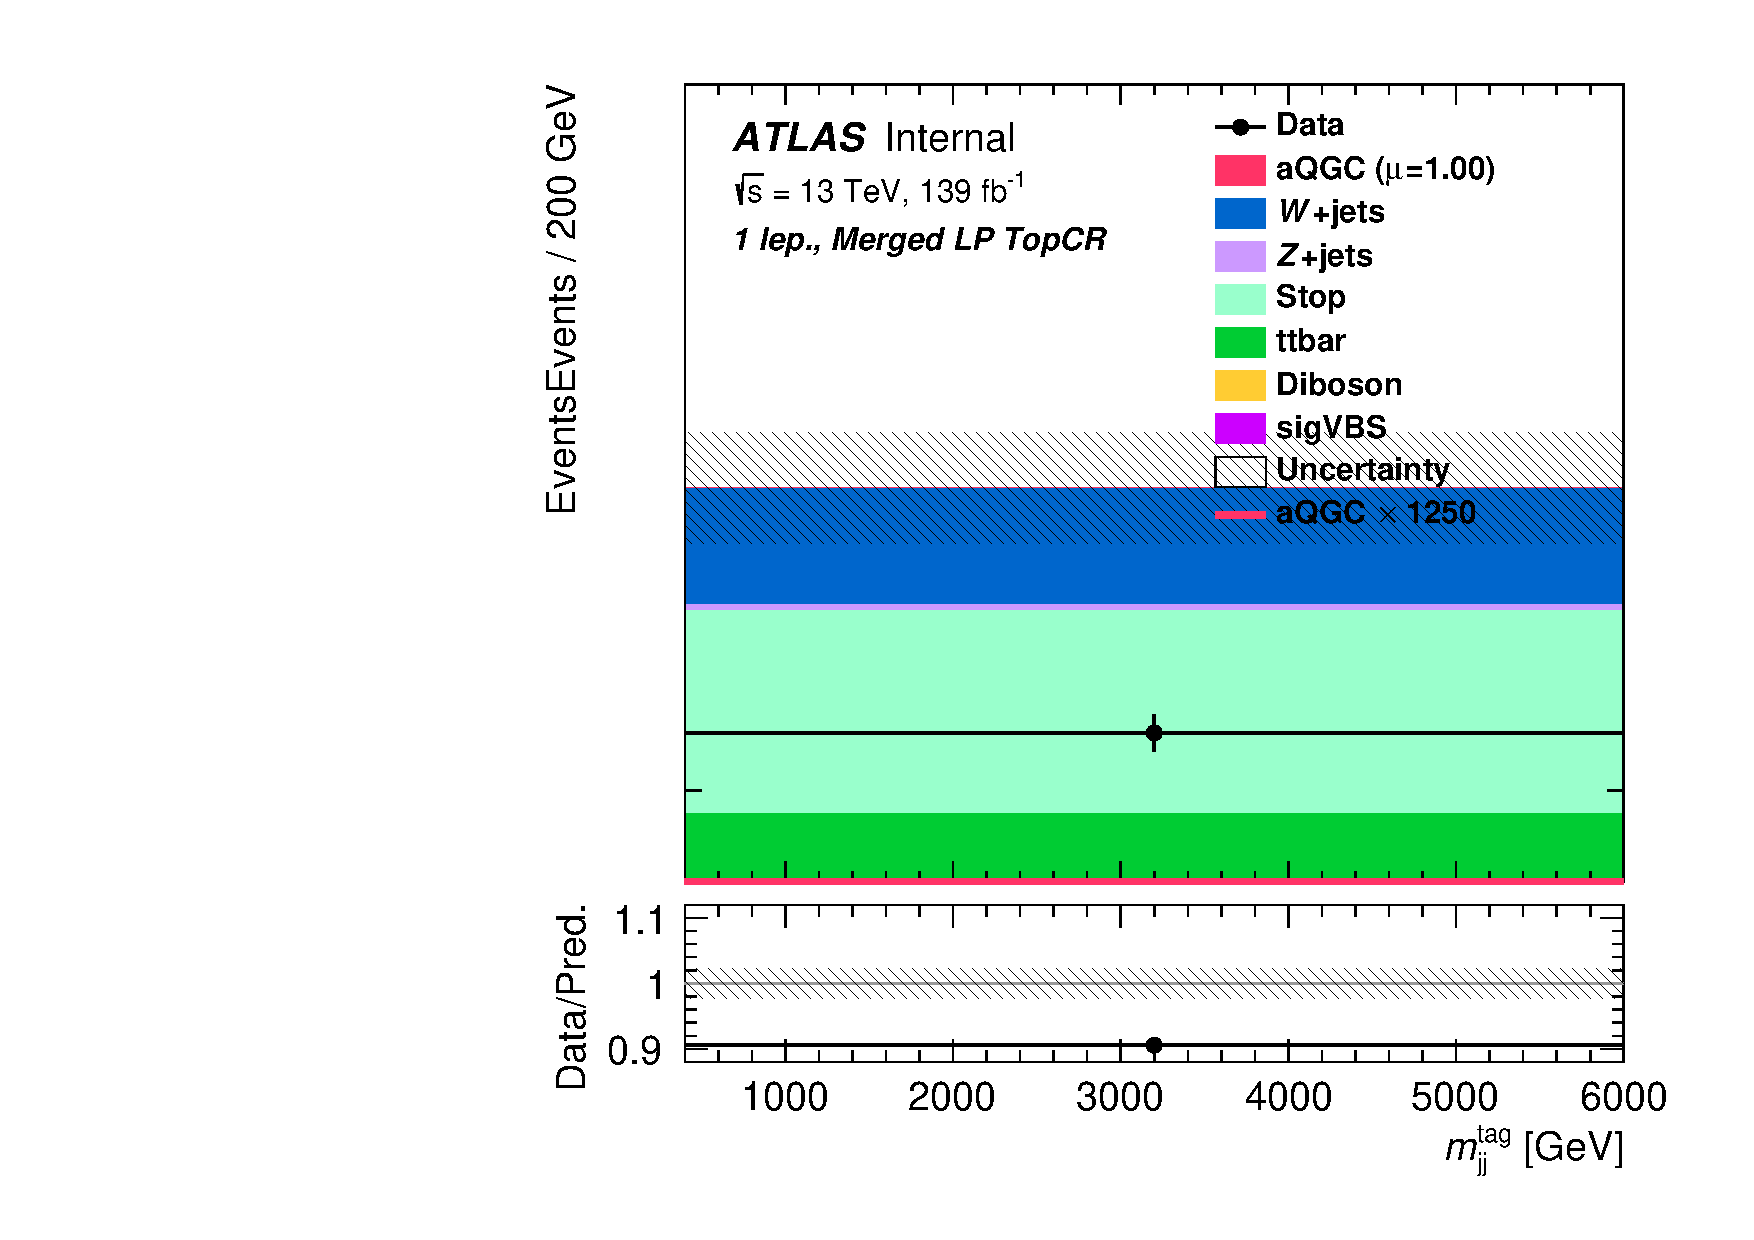
\includegraphics[width=0.35\textwidth]{figures/aQGC/Region_disttagMjj_DCRTopLP_BMin0_J0_incJet1_L1_T0_incFat1_Y6051_incTag1_Fat1_Prefitlog.pdf}
    	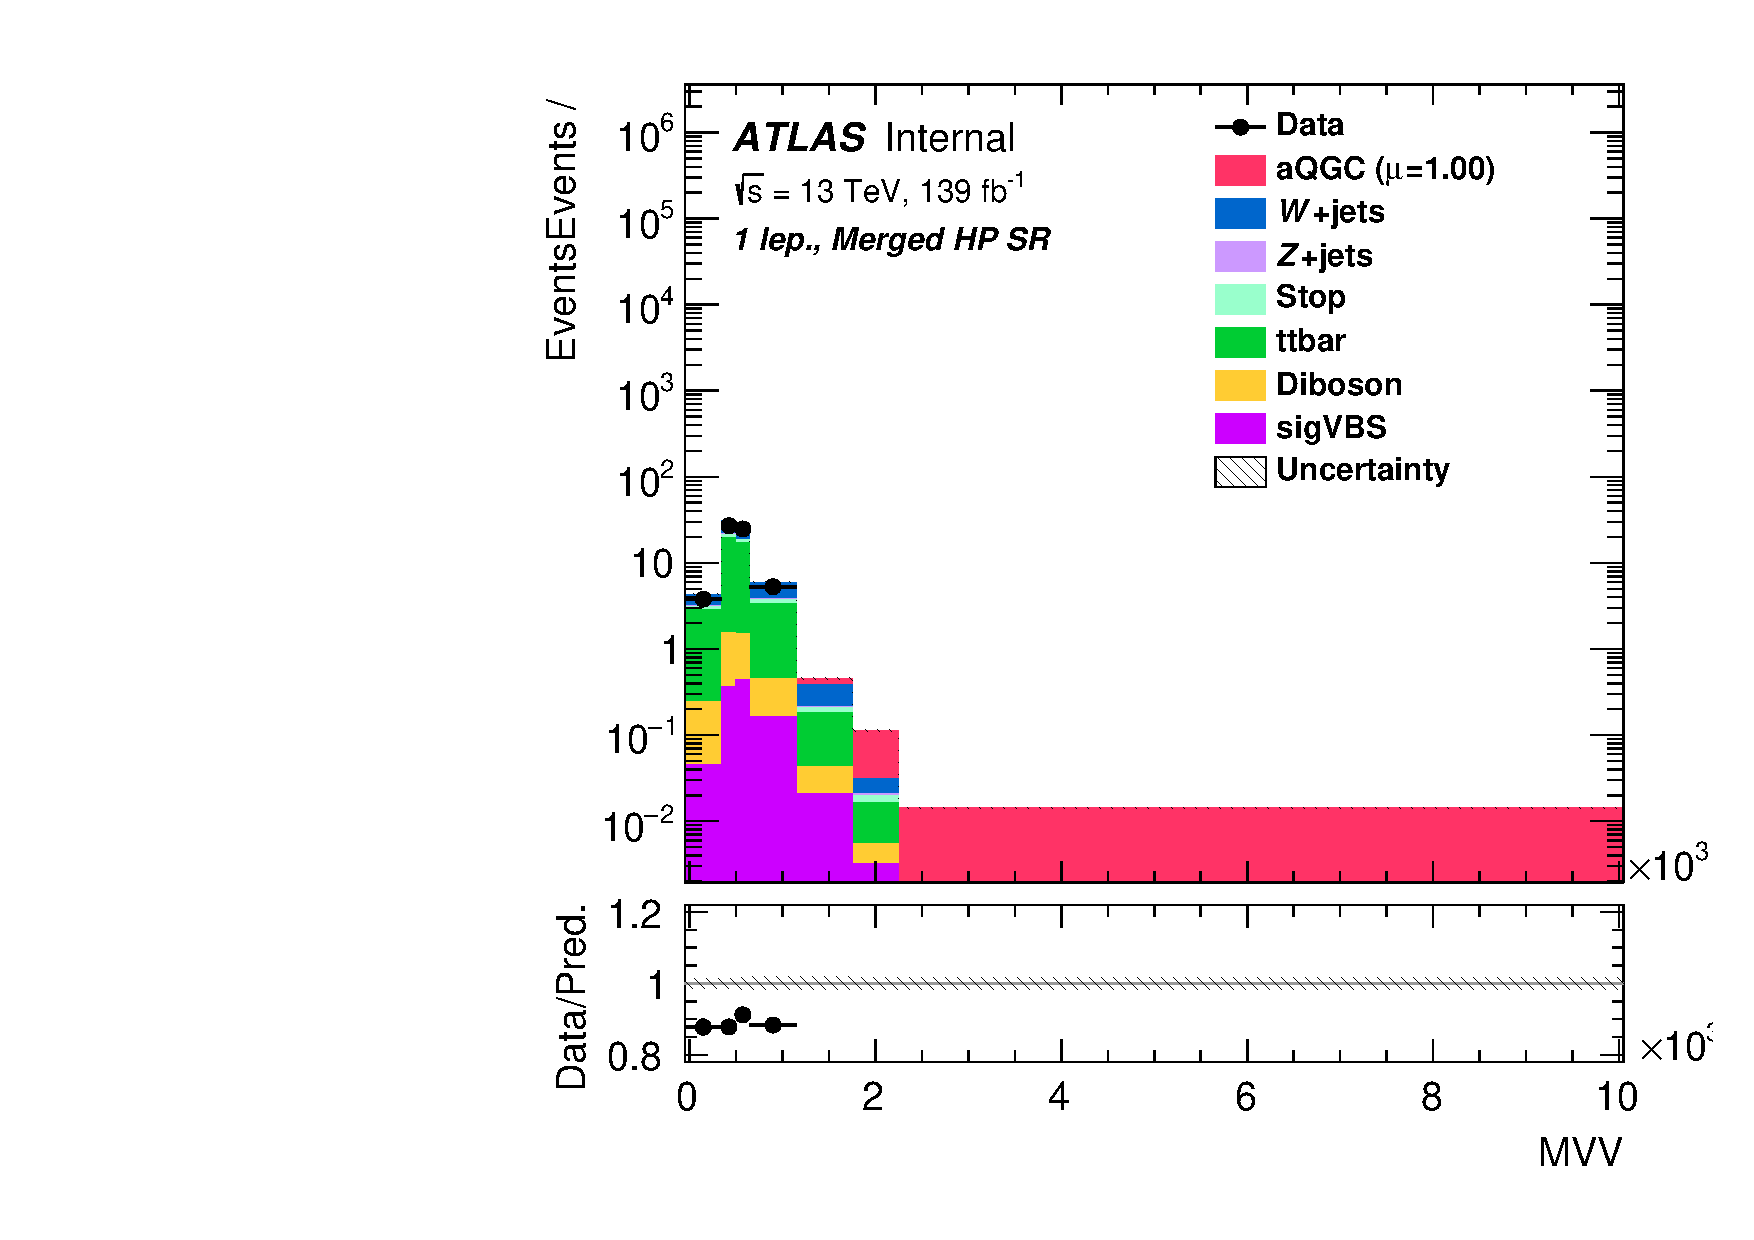
\includegraphics[width=0.35\textwidth]{figures/aQGC/Region_distMVV_DSRVBSHP_BMin0_J0_incJet1_L1_T0_incFat1_Y6051_incTag1_Fat1_Prefitlog.pdf}
    	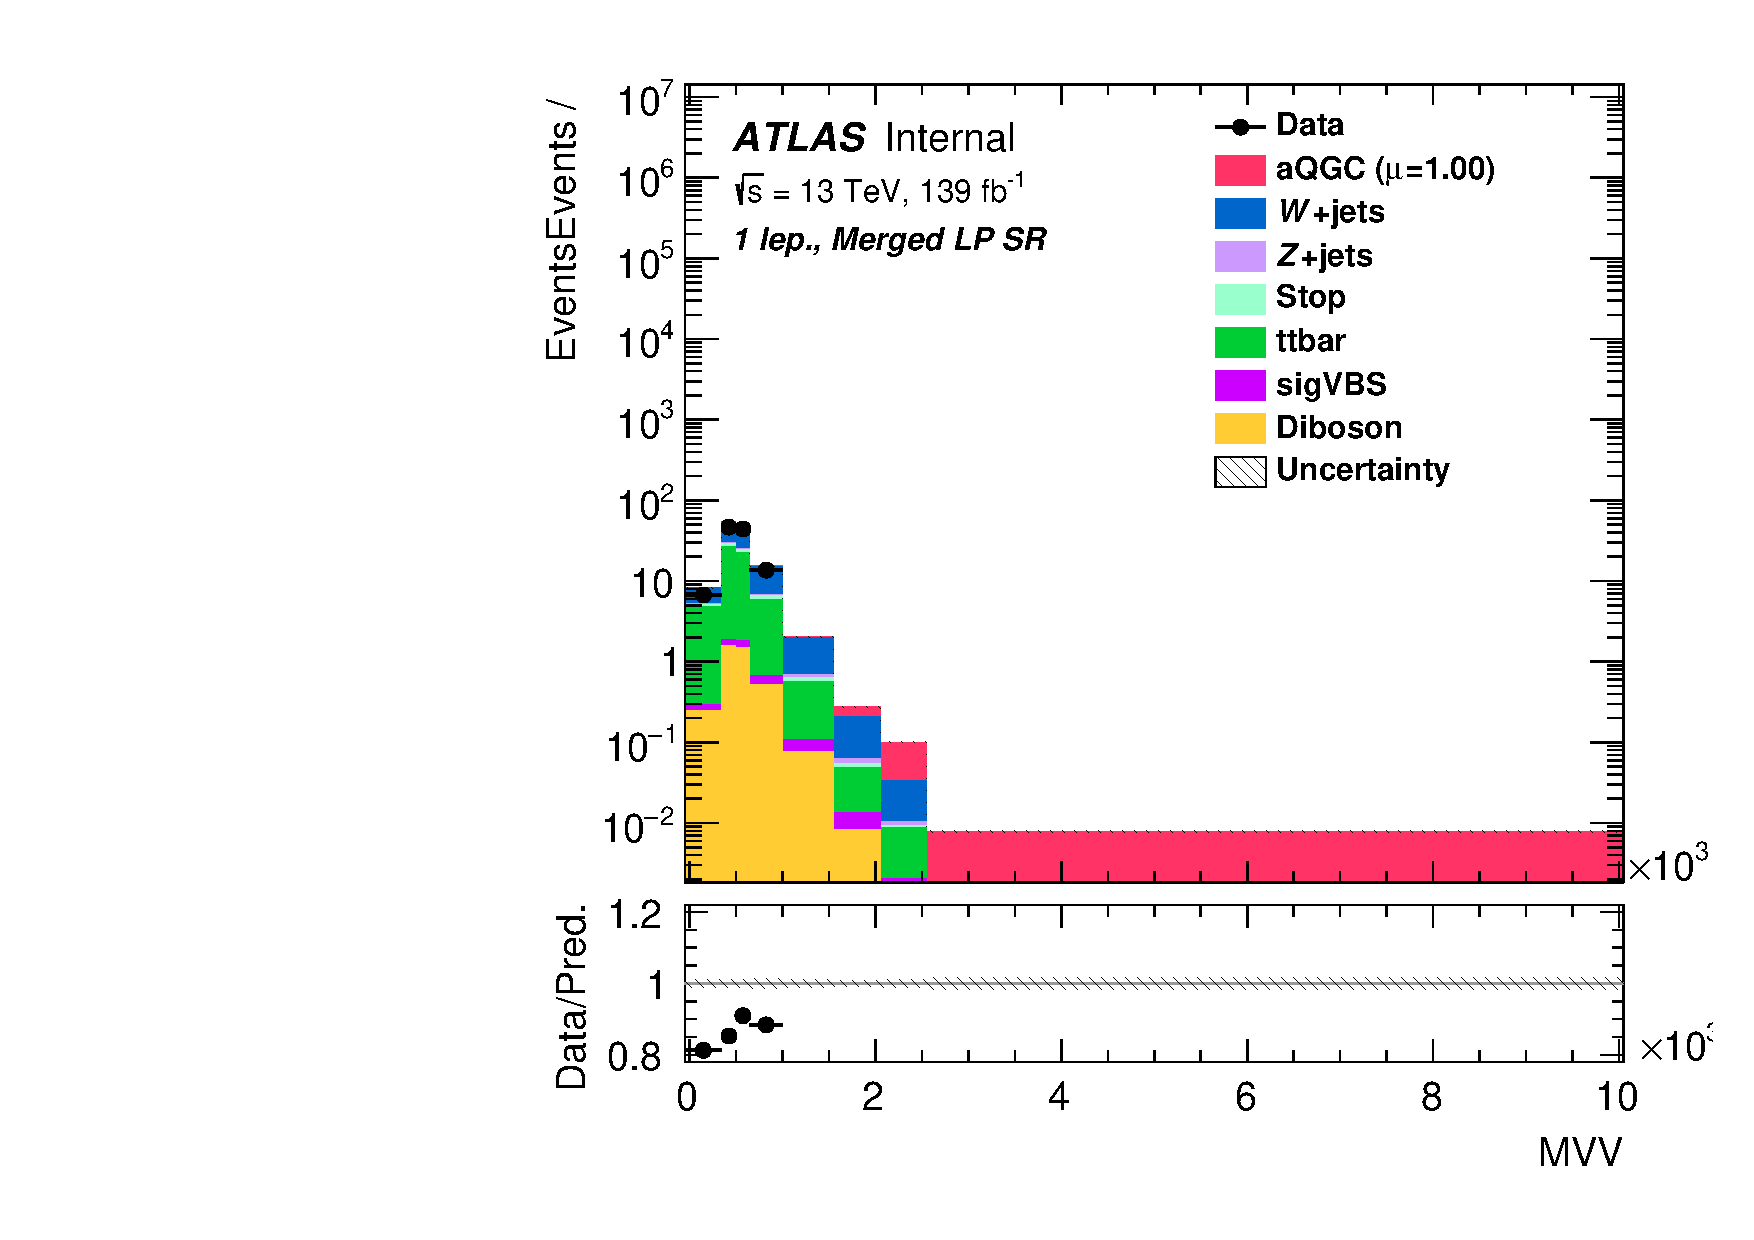
\includegraphics[width=0.35\textwidth]{figures/aQGC/Region_distMVV_DSRVBSLP_BMin0_J0_incJet1_L1_T0_incFat1_Y6051_incTag1_Fat1_Prefitlog.pdf}
    	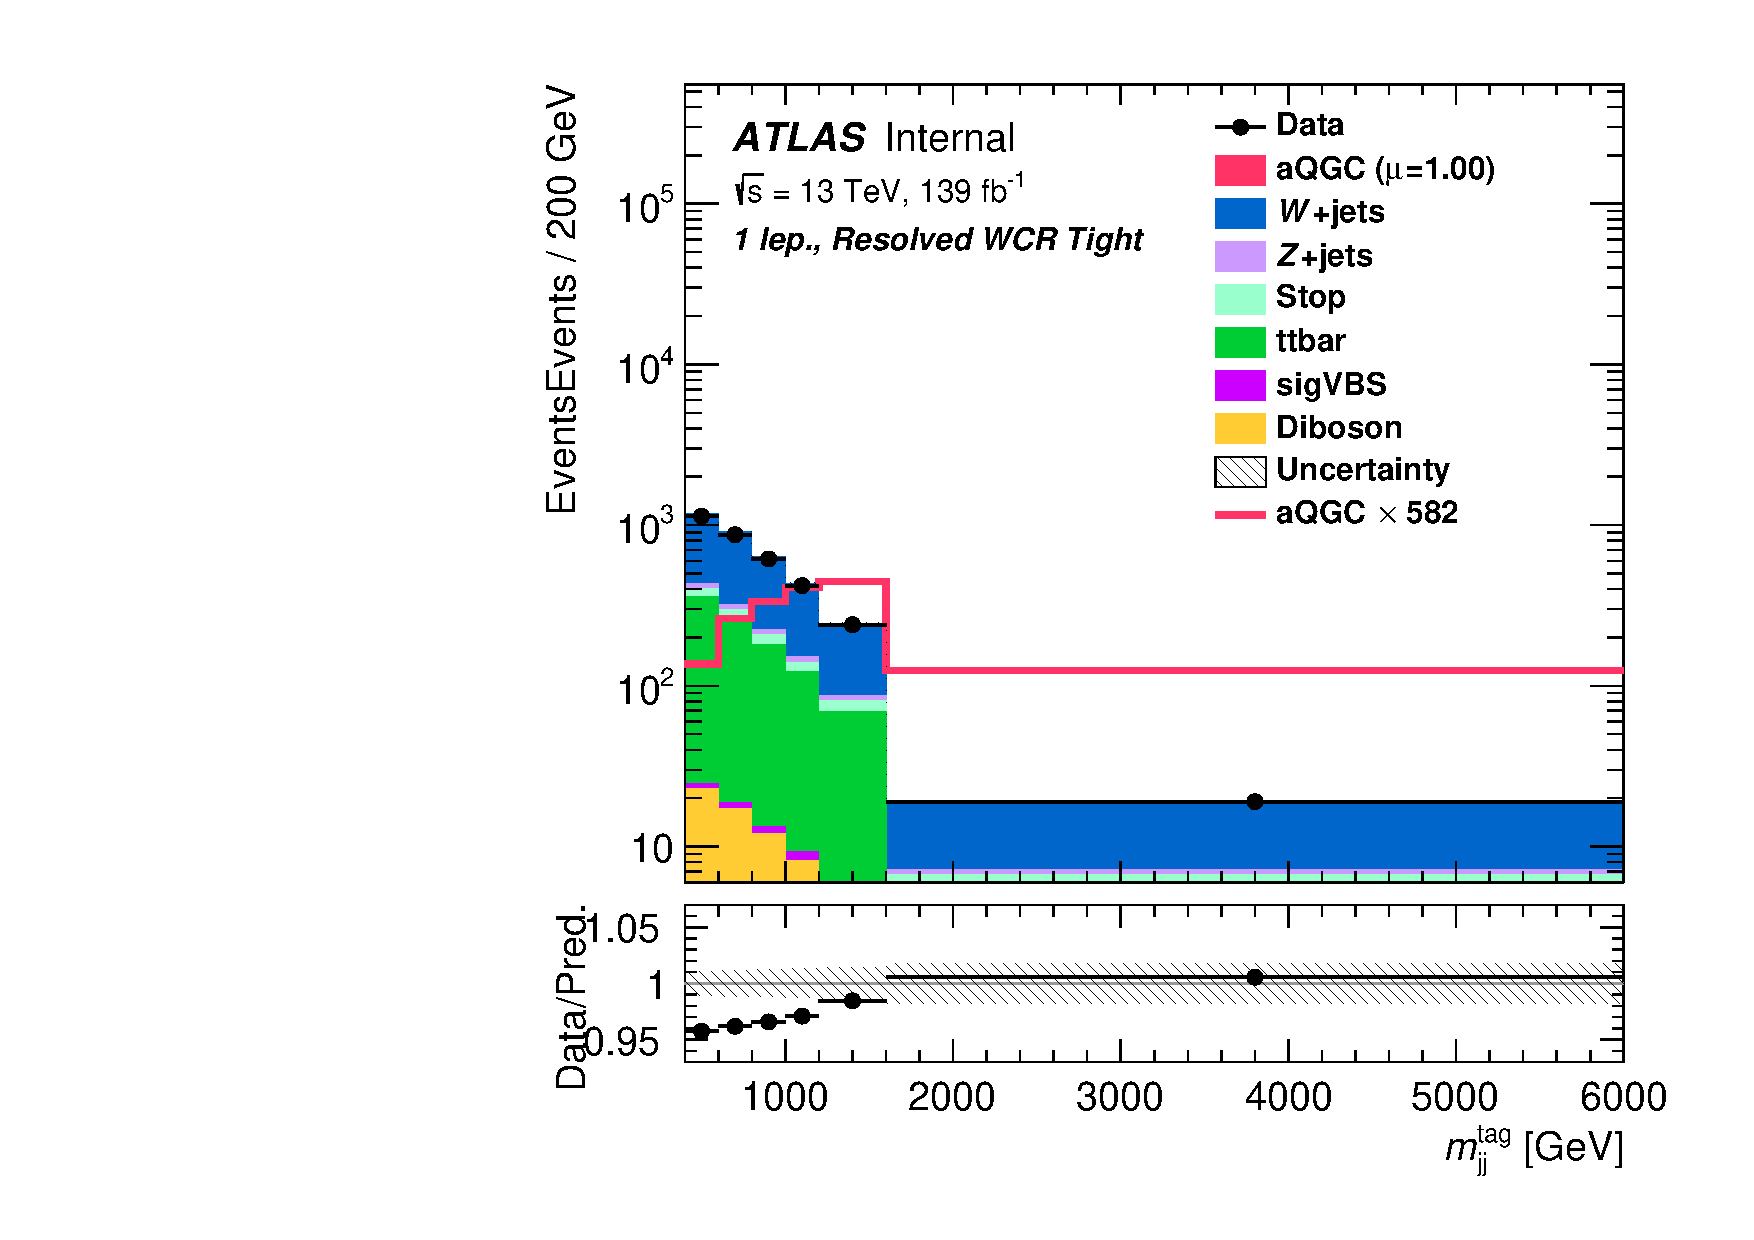
\includegraphics[width=0.35\textwidth]{figures/aQGC/Region_disttagMjj_DCRVjetTight_BMin0_T0_Y6051_incTag1_J2_L1_incJet1_Prefitlog.pdf}
    	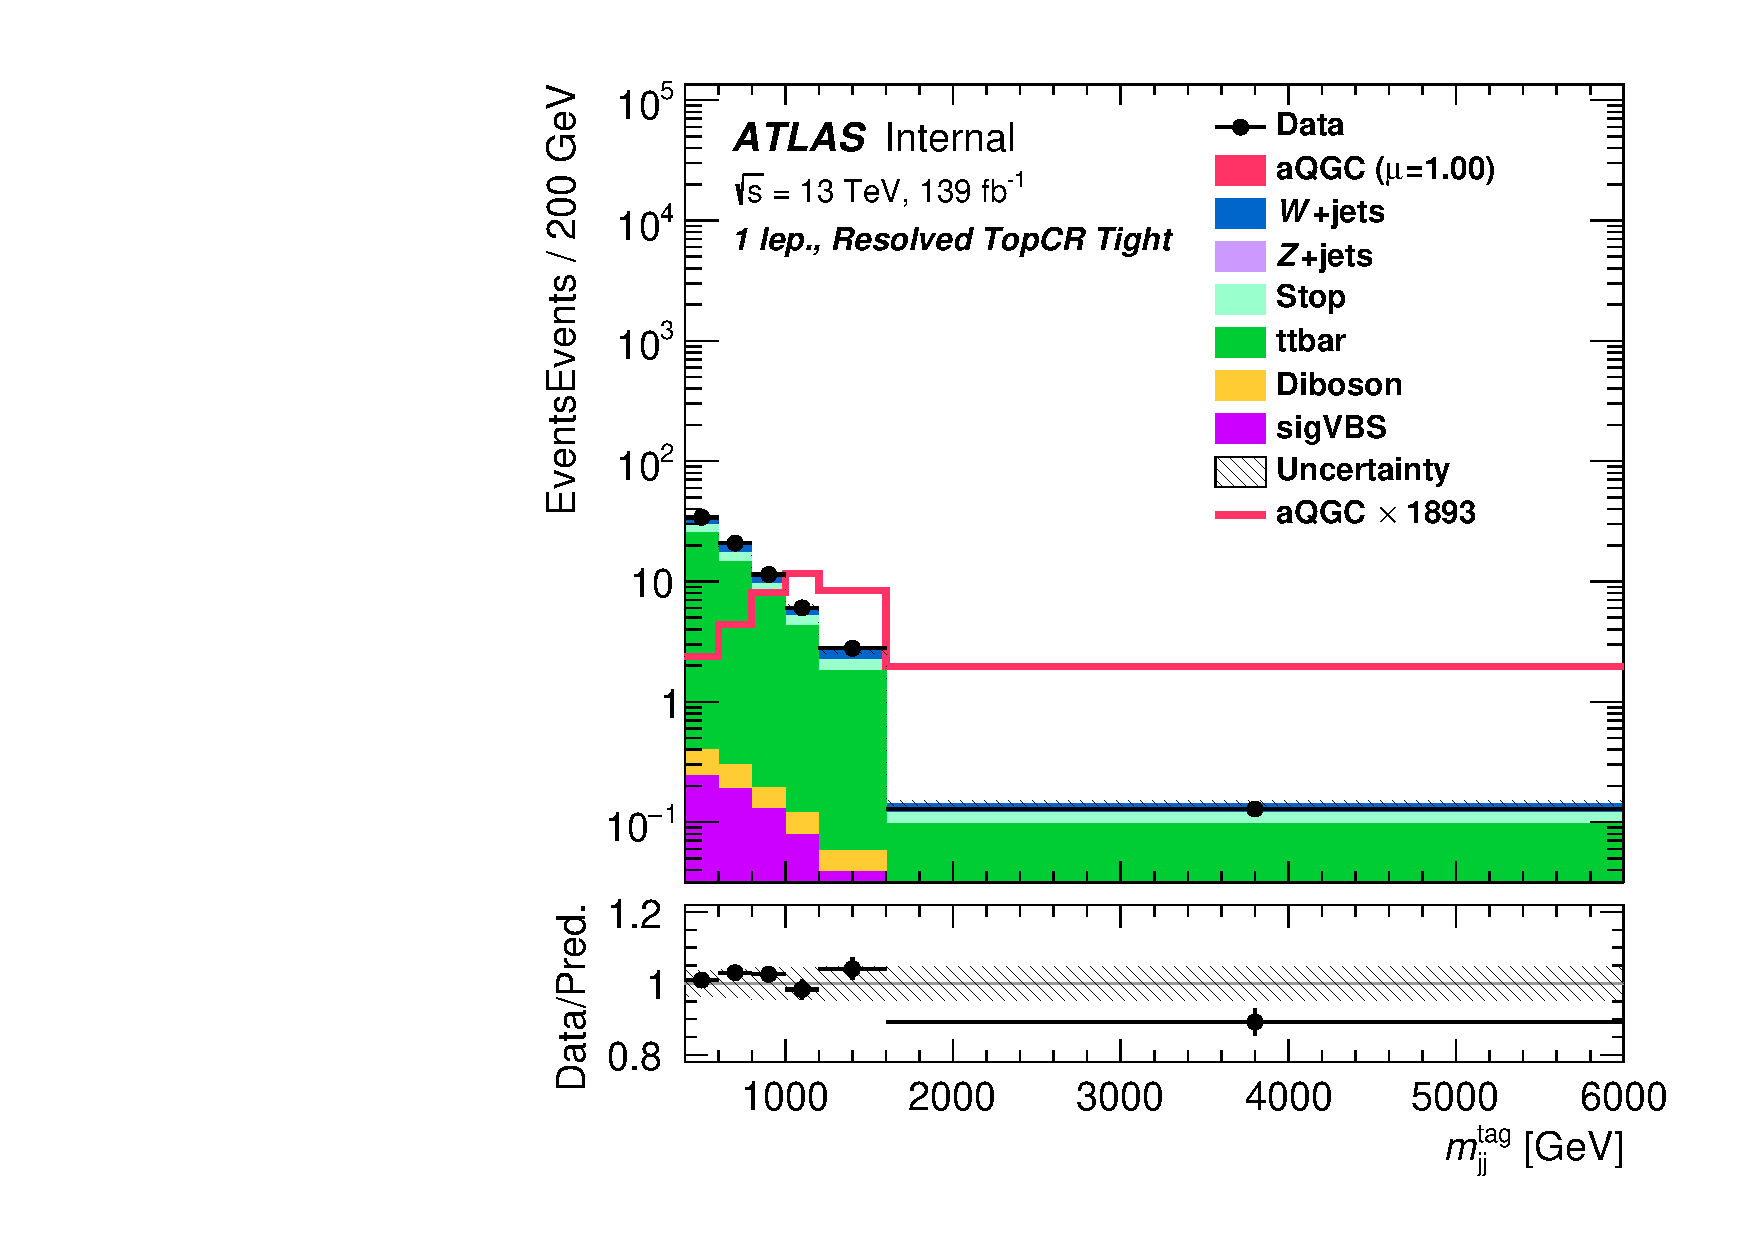
\includegraphics[width=0.35\textwidth]{figures/aQGC/Region_disttagMjj_DCRTopTight_BMin0_T0_Y6051_incTag1_J2_L1_incJet1_Prefitlog.pdf}
    	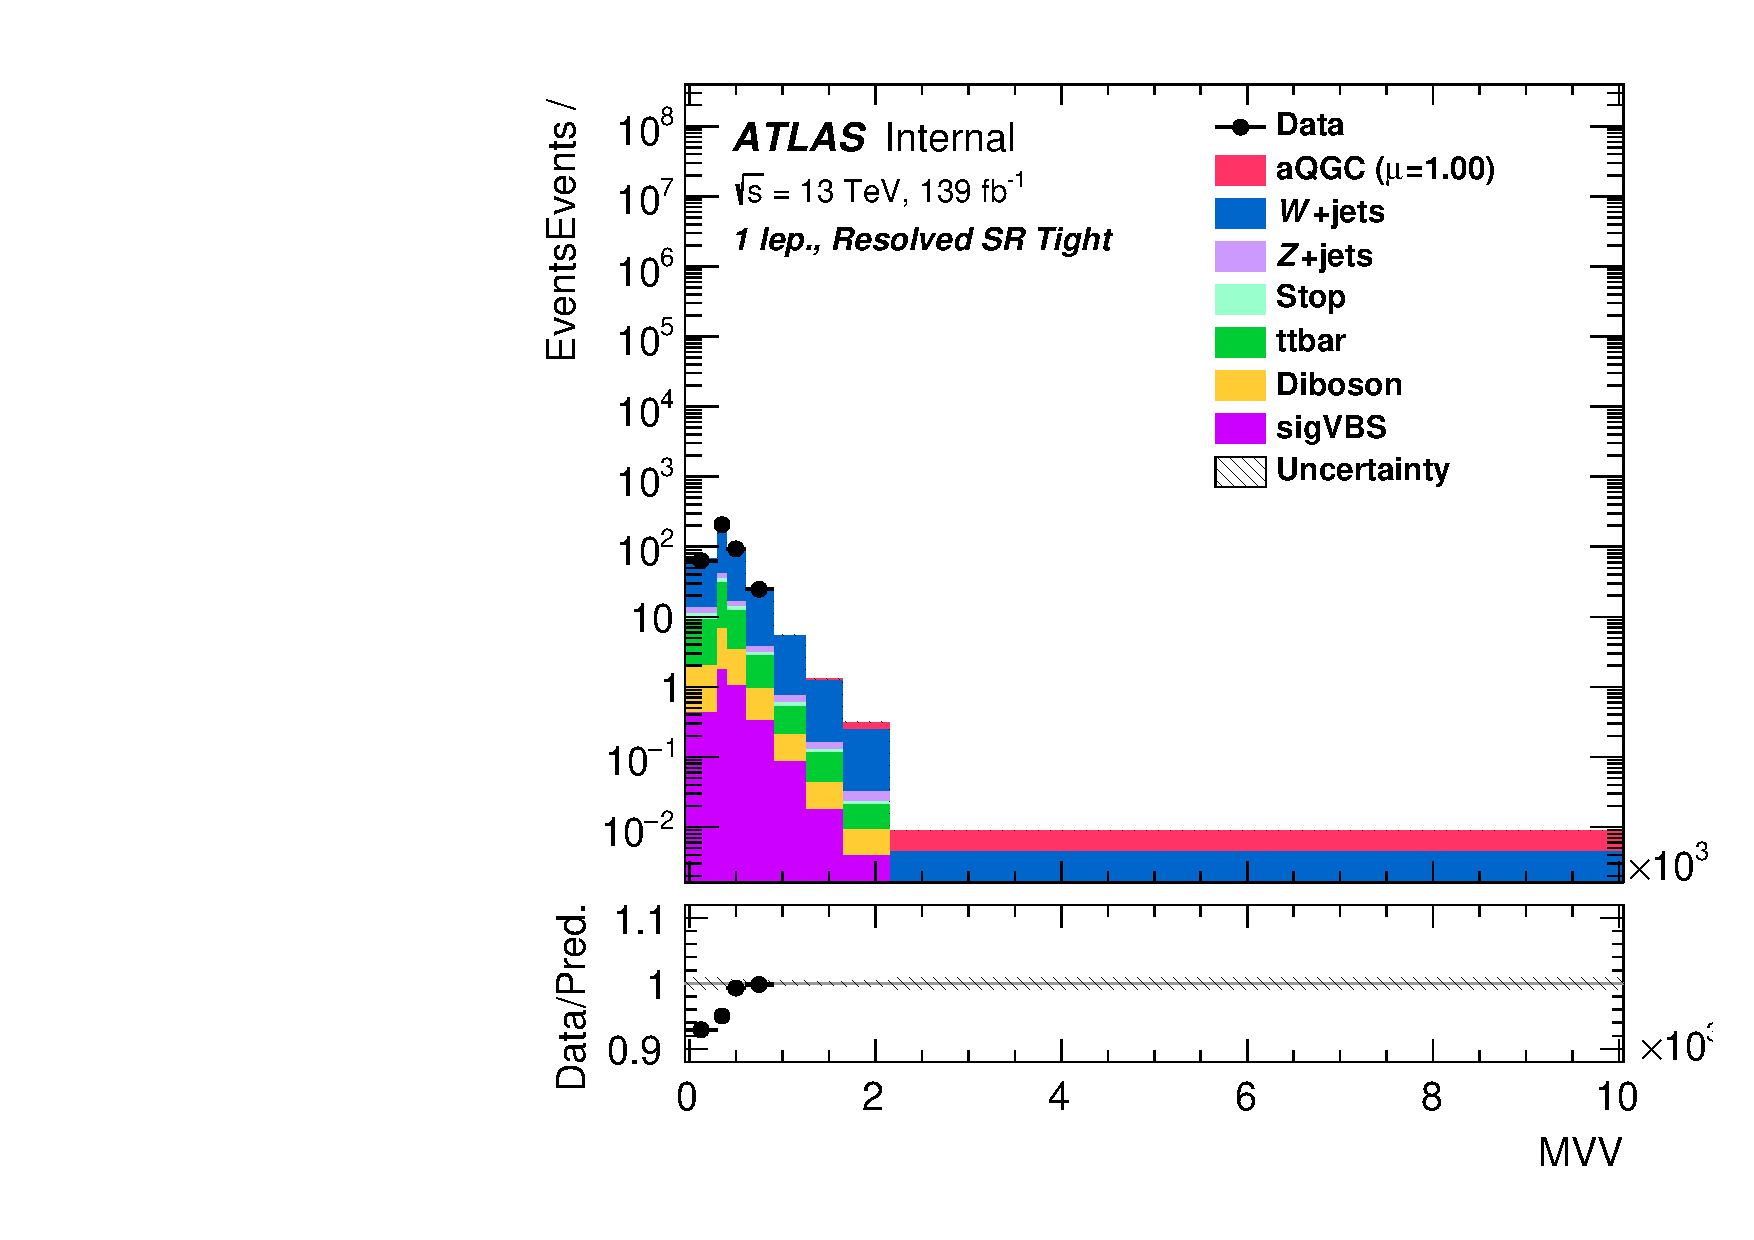
\includegraphics[width=0.35\textwidth]{figures/aQGC/Region_distMVV_DSRVBSTight_BMin0_T0_Y6051_incTag1_J2_L1_incJet1_Prefitlog.pdf}
        \caption{Prefit plots for operator FT0 in \olep channel are shown. The standard model EW signal is floated as the background.}
        \label{fig:1lepFT0}
\end{figure}

\begin{figure}[ht]
    \centering
    	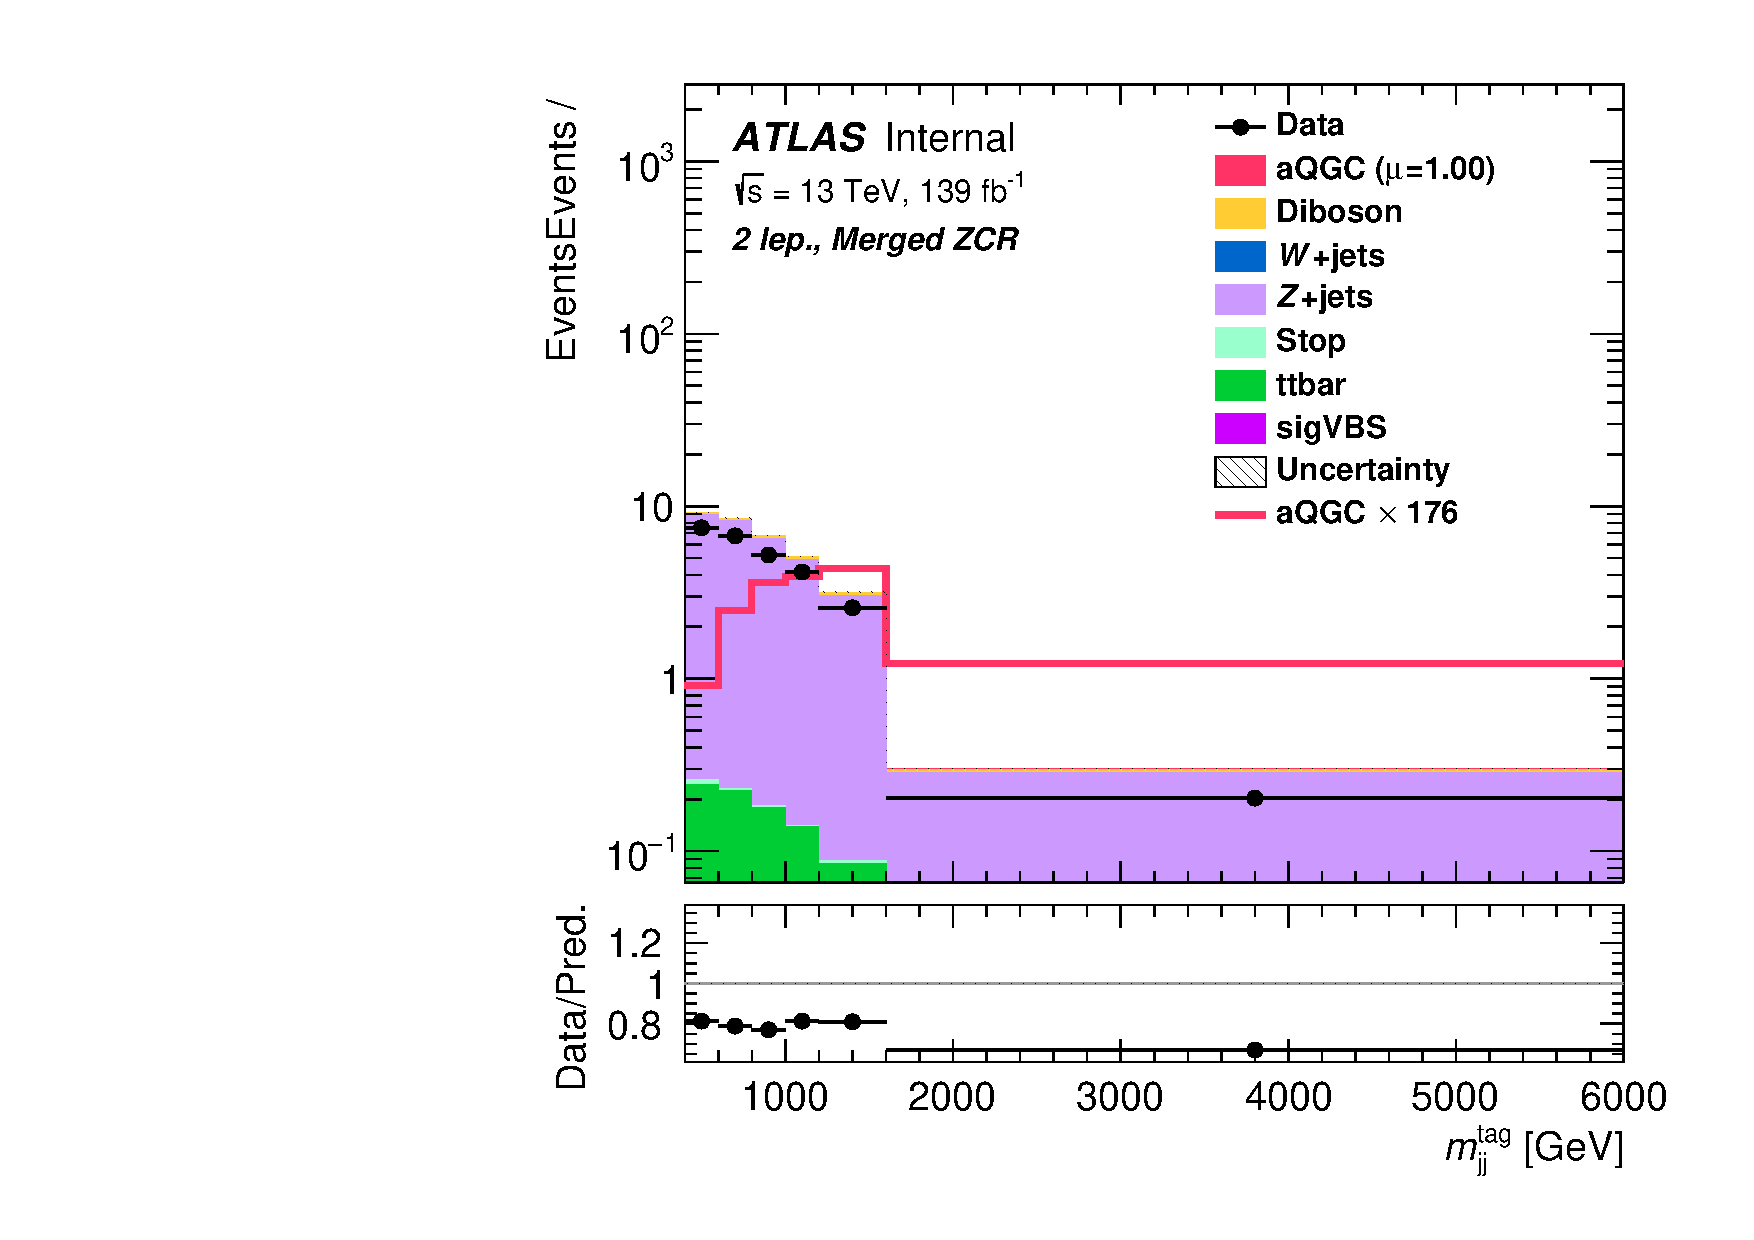
\includegraphics[width=0.35\textwidth]{figures/aQGC/Region_distMTagMerJets_DCRVjet_BMin0_J0_incJet1_L2_T0_incFat1_Y6051_incTag1_Fat1_Prefitlog.pdf}
    	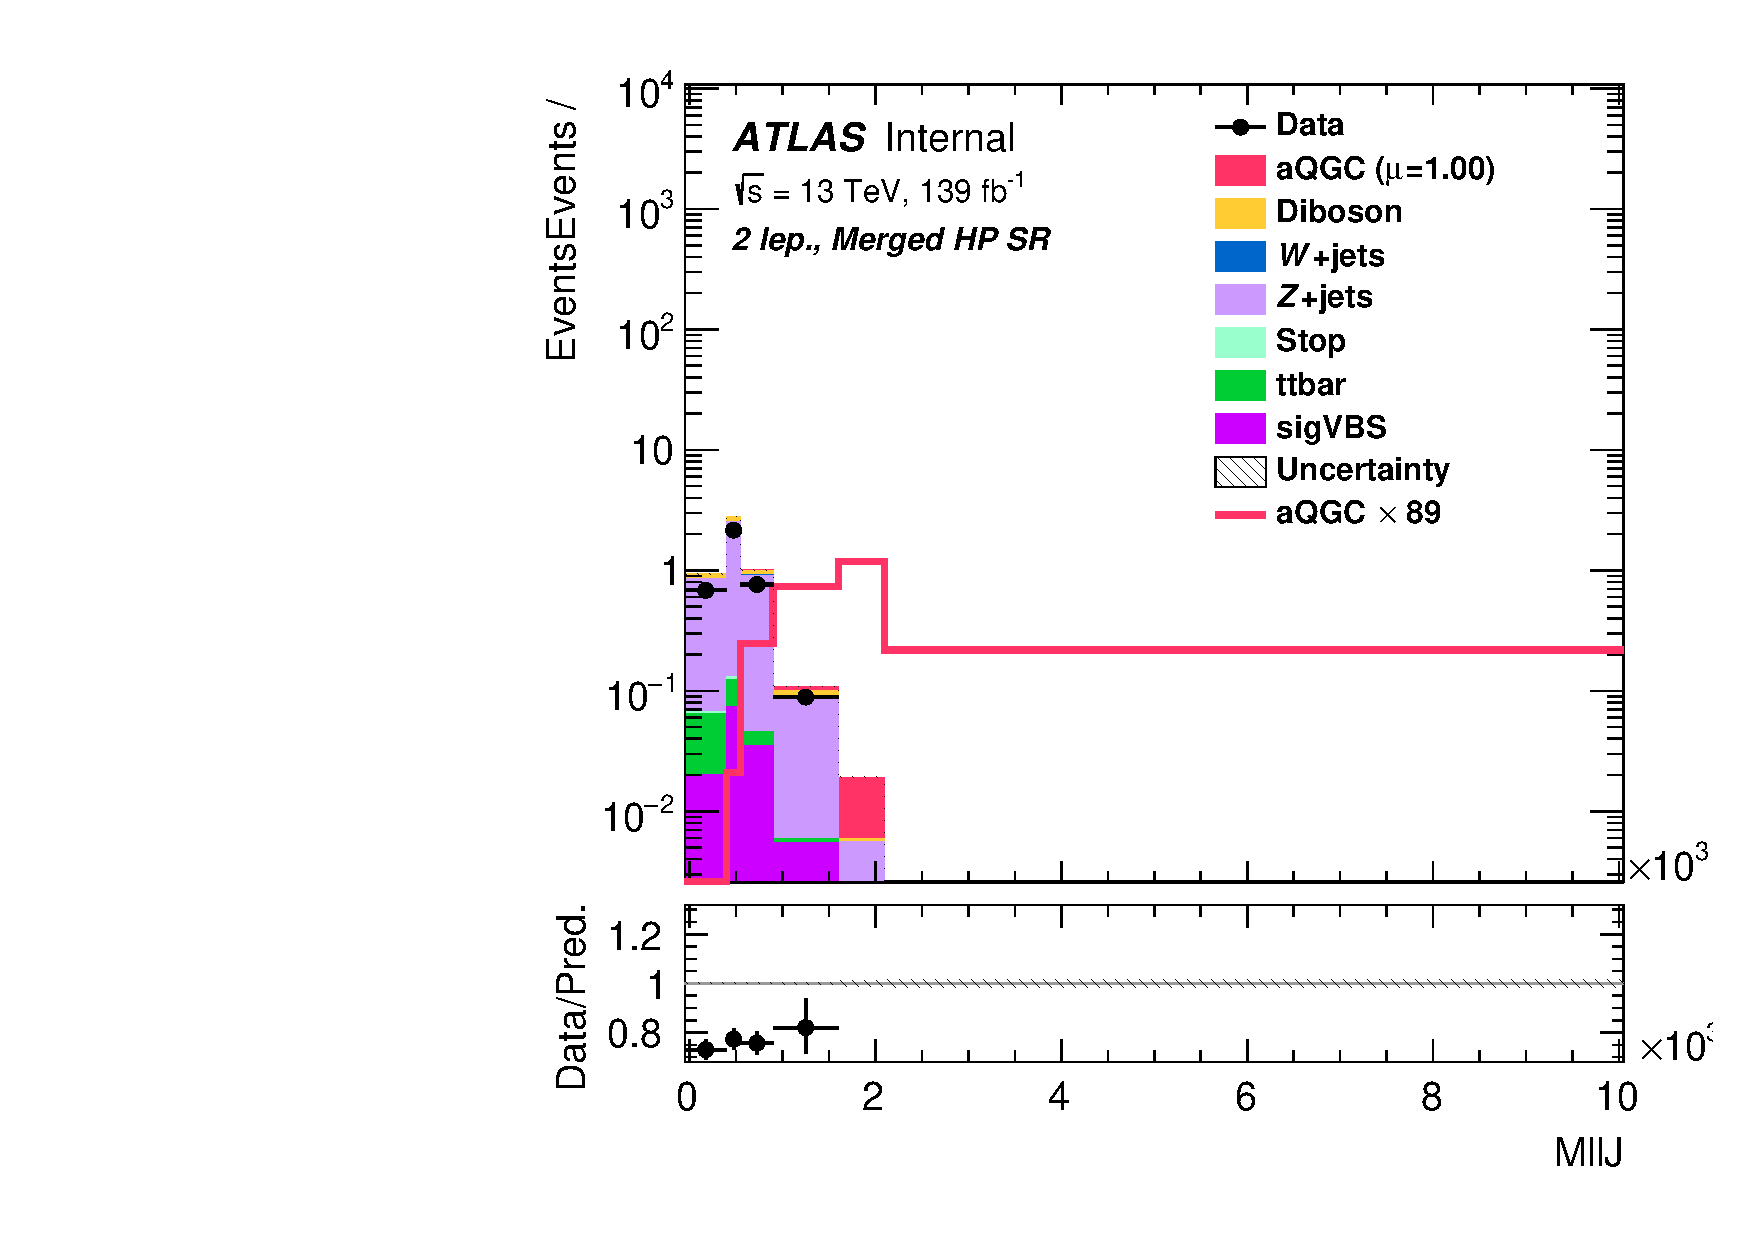
\includegraphics[width=0.35\textwidth]{figures/aQGC/Region_distMllJ_DSRVBSHP_BMin0_J0_incJet1_L2_T0_incFat1_Y6051_incTag1_Fat1_Prefitlog.pdf}
    	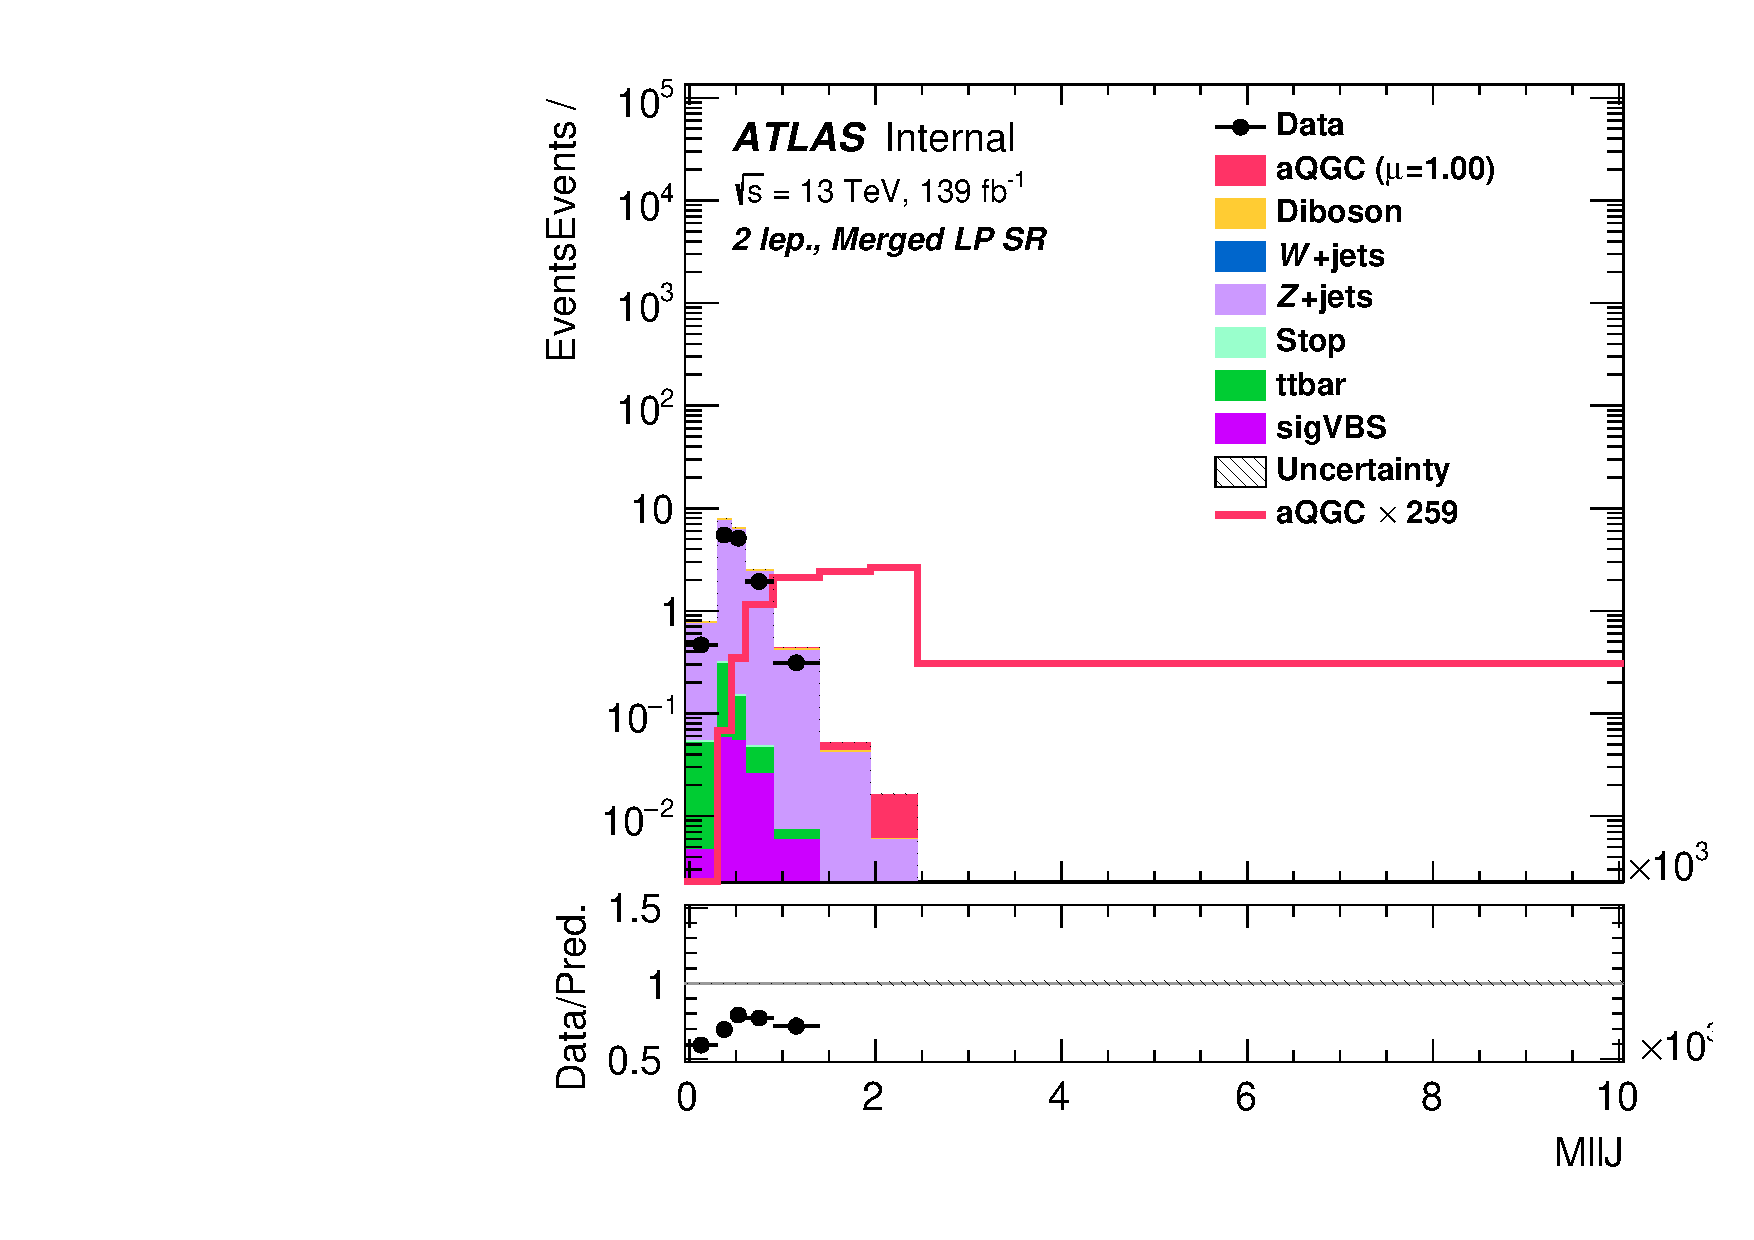
\includegraphics[width=0.35\textwidth]{figures/aQGC/Region_distMllJ_DSRVBSLP_BMin0_J0_incJet1_L2_T0_incFat1_Y6051_incTag1_Fat1_Prefitlog.pdf}
    	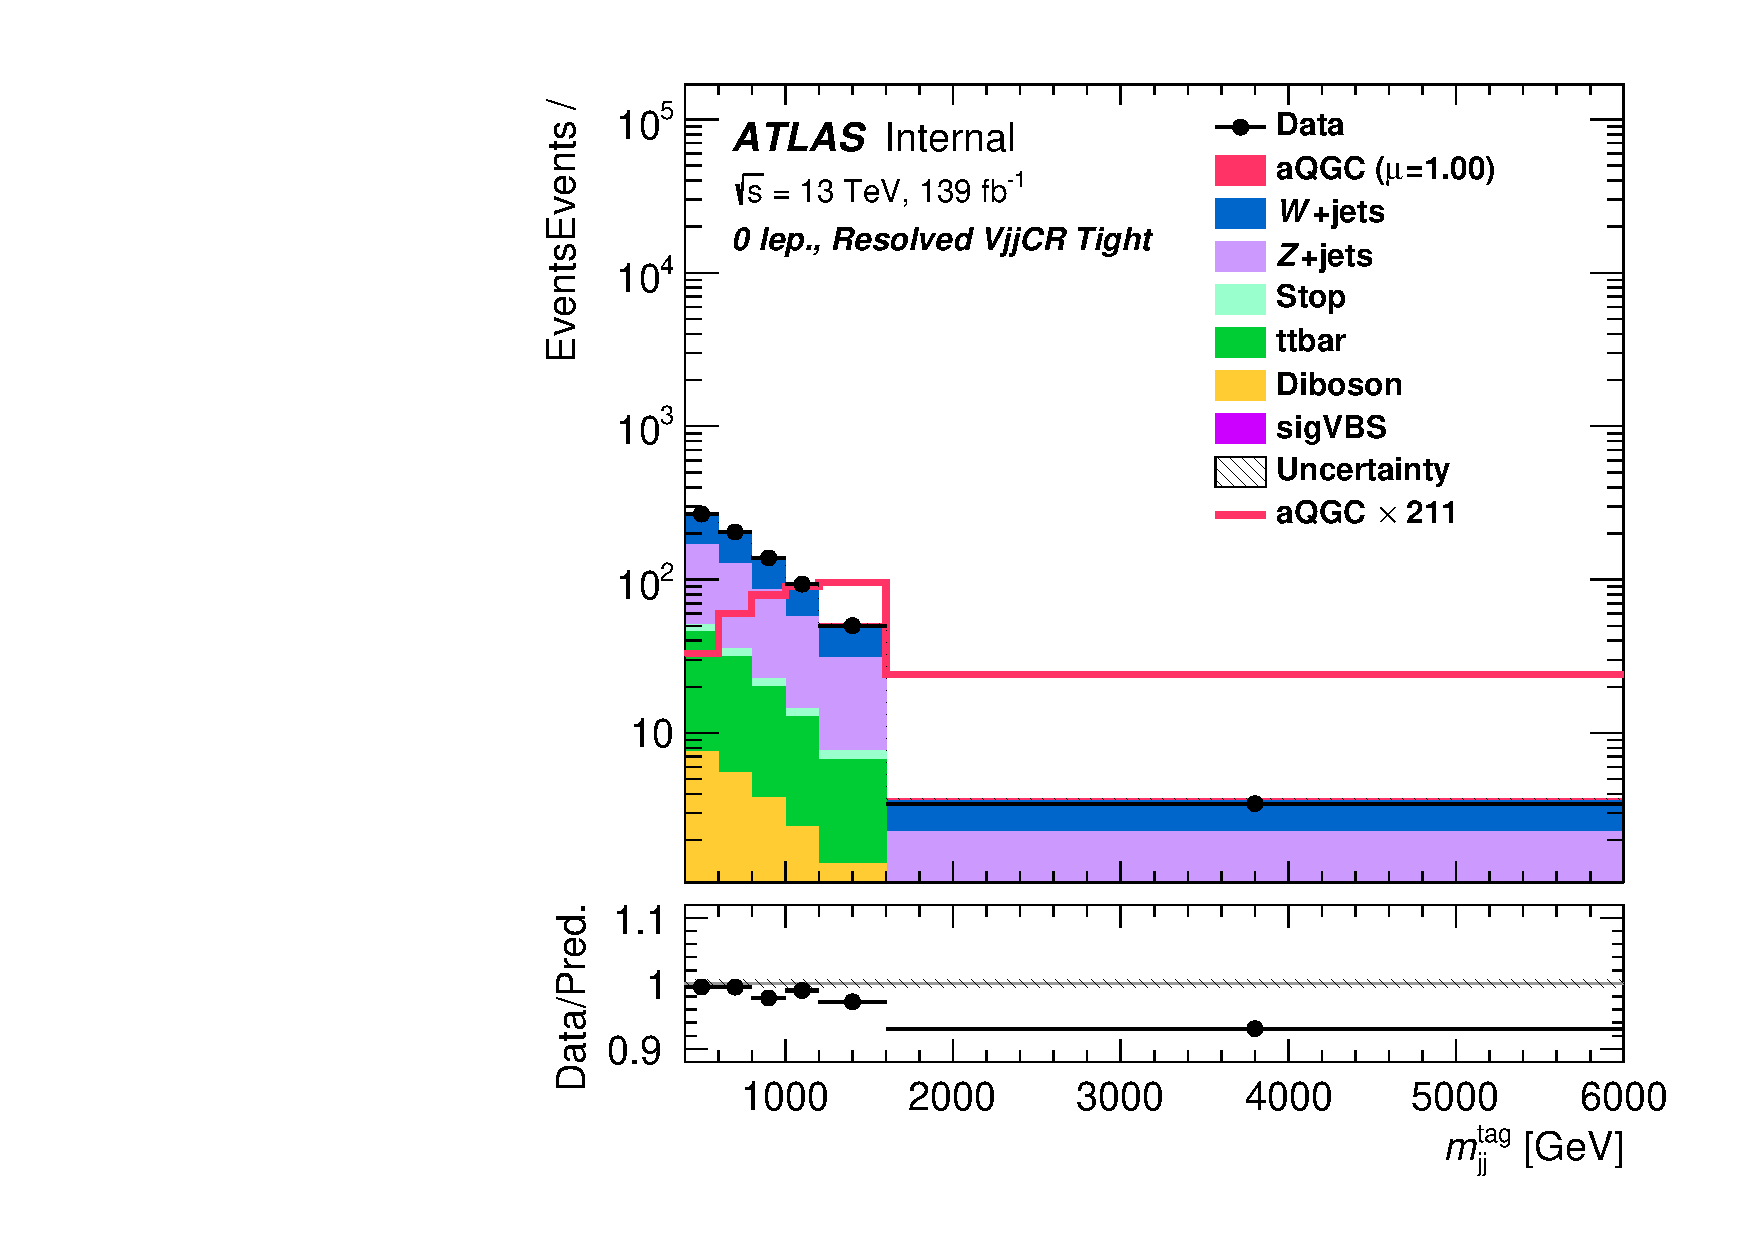
\includegraphics[width=0.35\textwidth]{figures/aQGC/Region_distMTagJets_DCRVjetFid_BMin0_T0_Y6051_incTag1_J2_L0_incJet1_Prefitlog.pdf}
    	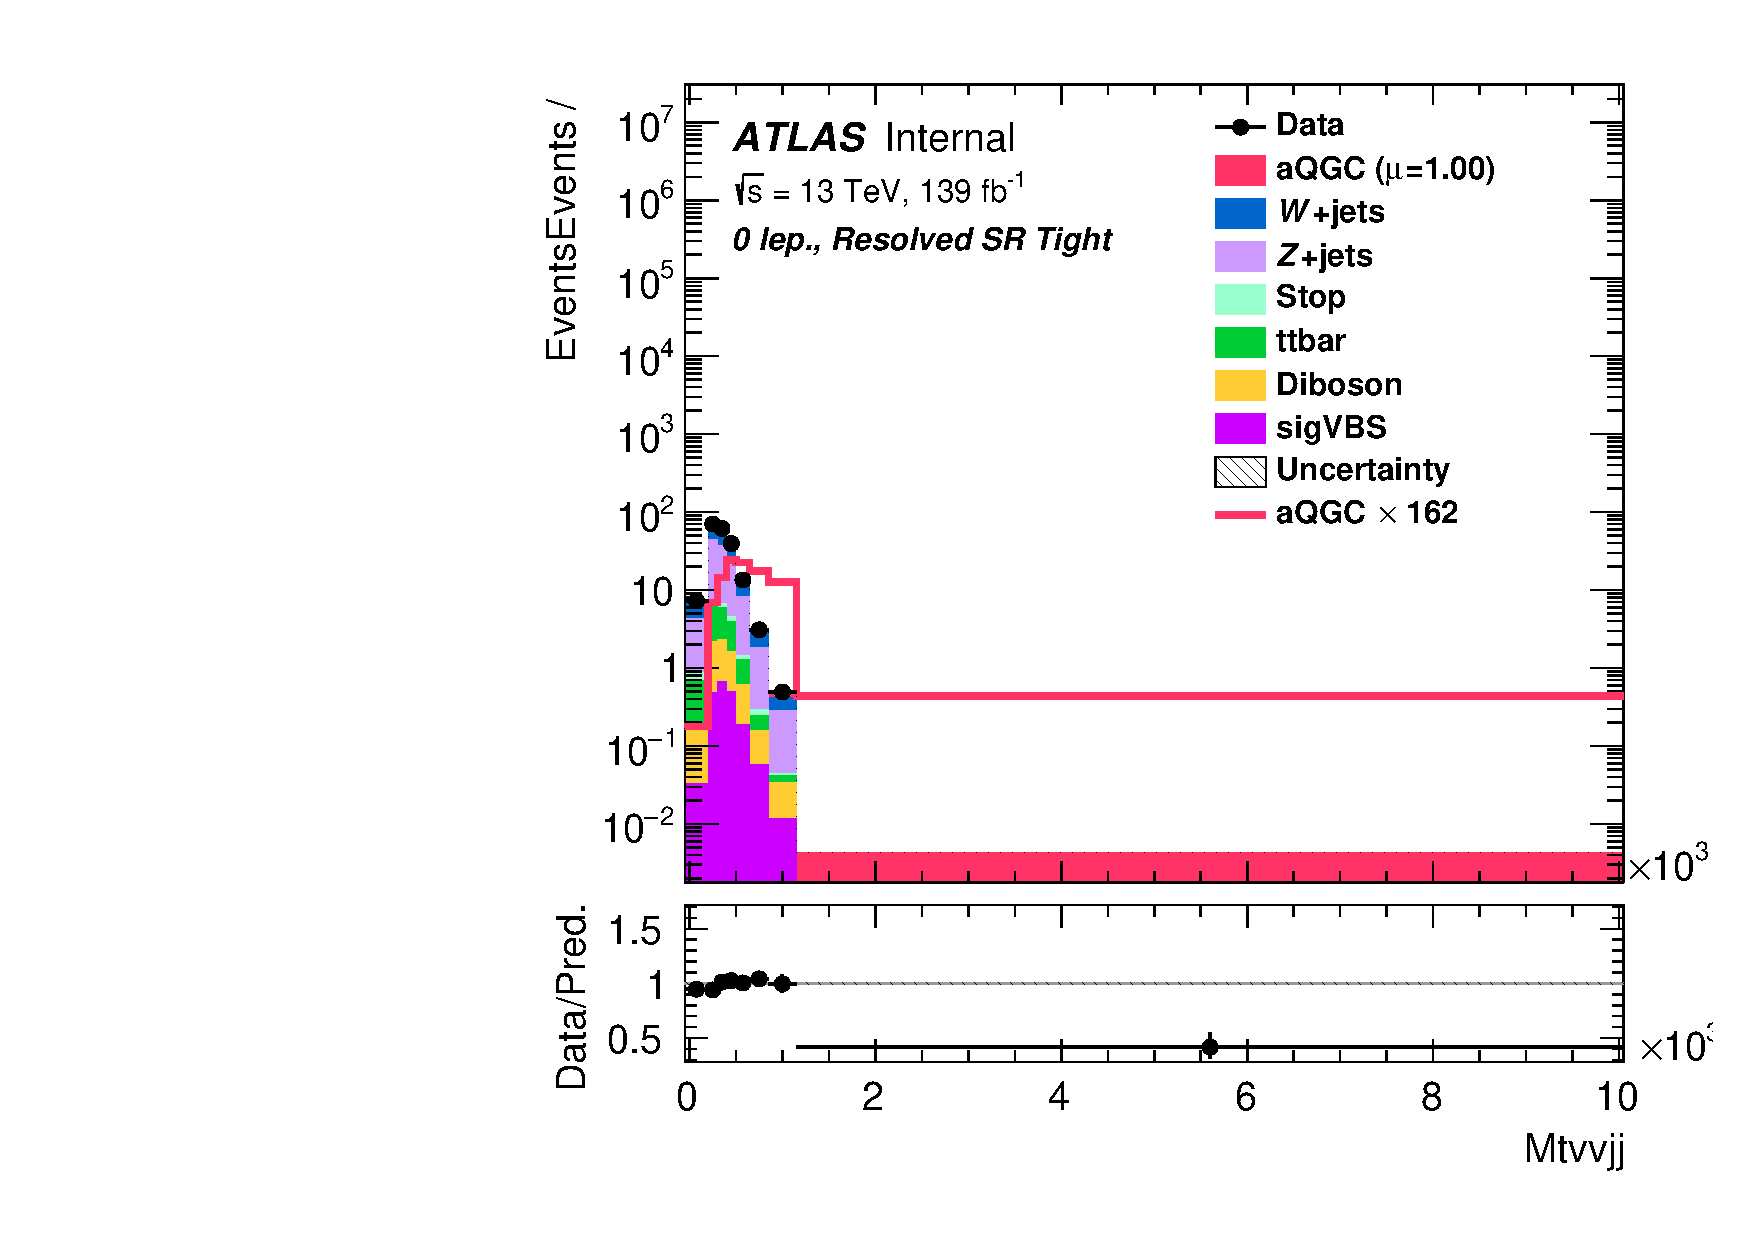
\includegraphics[width=0.35\textwidth]{figures/aQGC/Region_distMtvvjj_DSRVBSFid_BMin0_T0_Y6051_incTag1_J2_L0_incJet1_Prefitlog.pdf}
        \caption{Prefit plots for operator FT0 in \tlep channel are shown. The standard model EW signal is floated as the background.}
        \label{fig:2lepFT0}
\end{figure}


\section{Clipping method}
\label{subsec:clipping}
As the EFT violates unitarity at large energy scale, the clipping method is used to preserve the unitarity at high center-of-mass energies. In order to guarantee that the extracted limit does not exceed valid energy scales, the EFT signal is set to zero at truth$m_{VV} > E_{clip}$, where the $E_{clip}$ is [2,3,4,5,$\infty$]~TeV. 5 points are chosen as recommended from the aGC coupling taskforce.\cite{ATL-COM-PHYS-2017-433} 
The expected limit with all 3 channels with each of the clipping points are shown in figure~\ref{fig:ClippedLimits}. 
The all systematics uncertainties identical to the standard model fitting is included, thought they don't effect to the fitting results since at the tail of the diboson mass ($m_{VV}$) distribution where affects the sensitivity, the statistical uncertainties are dominant source of the uncertainty and the effect of the systematics uncertainty is not so large.

The unitarity bound can be calculated theoretically for each Wilson coefficient.
If the limits obtained by the experiment is lower than the limit calculated theoretically, it means the theoretical constraints are more strict than experiment can give. The calculated unitarity bound is overlaid in the Figure~\ref{}.

\section{Systematic interpretation}
The likelihood function is defined in the same way as the standard model fitting described in Chapter{}. According to the Wilk's theorem~\ref{}, the likelihood distribution asymptotically converges to a $\chi^2$ distribution. 
Therefore the $\chi^2$ distribution can be used to approximately estimate limits for $f/\Lambda^4$. For a 95\% level of confidence, the limits are derived as the boundaries of the corresponding interval of the $\chi^2$ distribution.
The limit on $f/\Rambda^4$ is directly obtained from the interval of the likelihood function. The interference term is accounted for the aQGC signal with the quadratic term by interpreting as $\mu_{QUAD} = \mu_{INT}^2$. 
The all limits in each clipping value are shown here. \\
%what's with the error of the obtained limit value??
\textcolor{red}{The following plots are to be replaced with CI ones}

\begin{figure}[ht]
    \centering
    	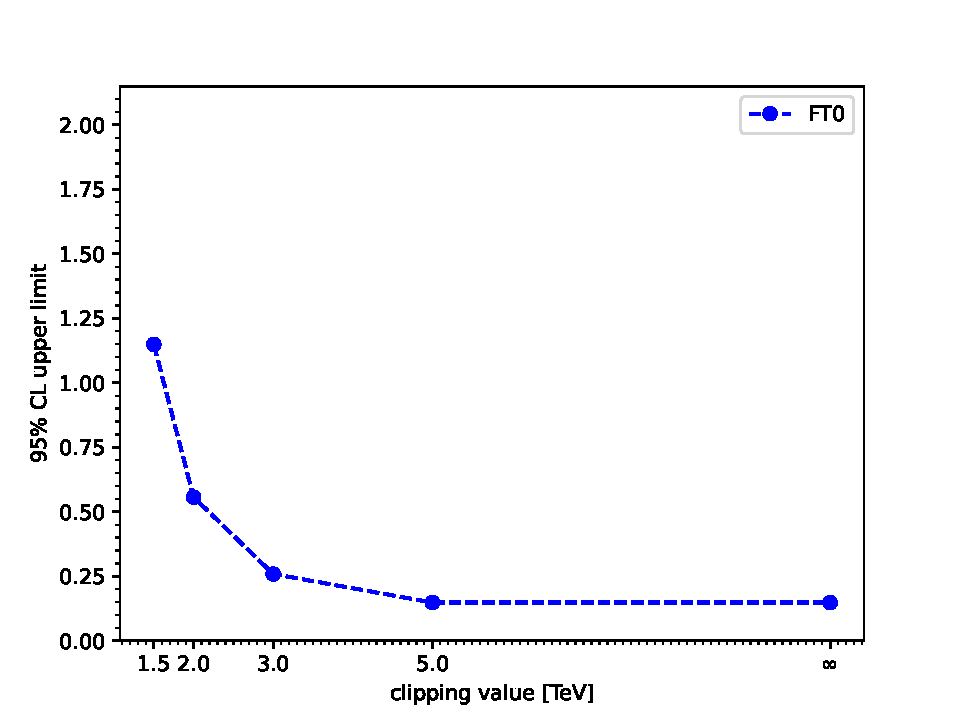
\includegraphics[width=0.35\textwidth]{figures/aQGC/ClippedFT0.pdf}
    	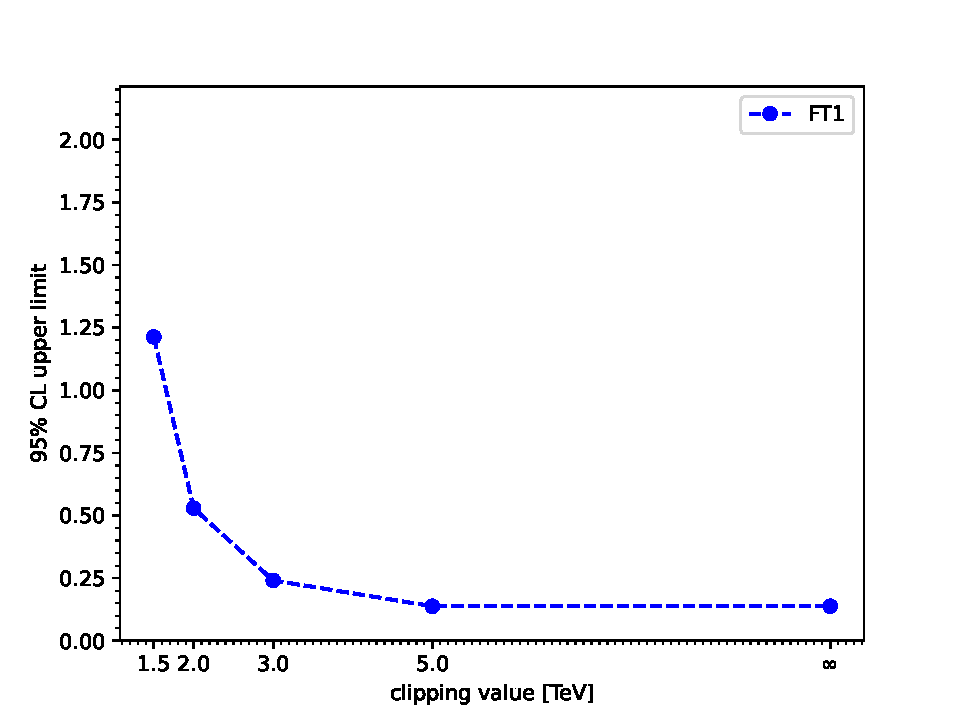
\includegraphics[width=0.35\textwidth]{figures/aQGC/ClippedFT1.pdf}
    	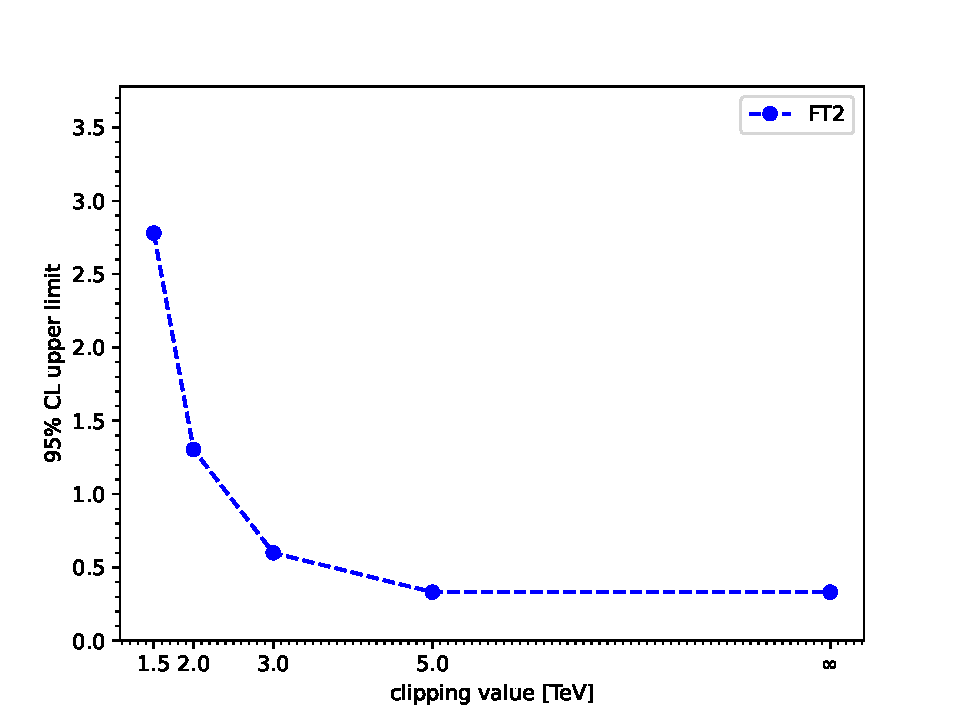
\includegraphics[width=0.35\textwidth]{figures/aQGC/ClippedFT2.pdf}
        \caption{Expected limits for 5 clipping points are shown for each coefficient FT0, FS02, and FM0.}
        \label{fig:ClippedLimits}
\end{figure}

\begin{figure}[ht]
    \centering
    	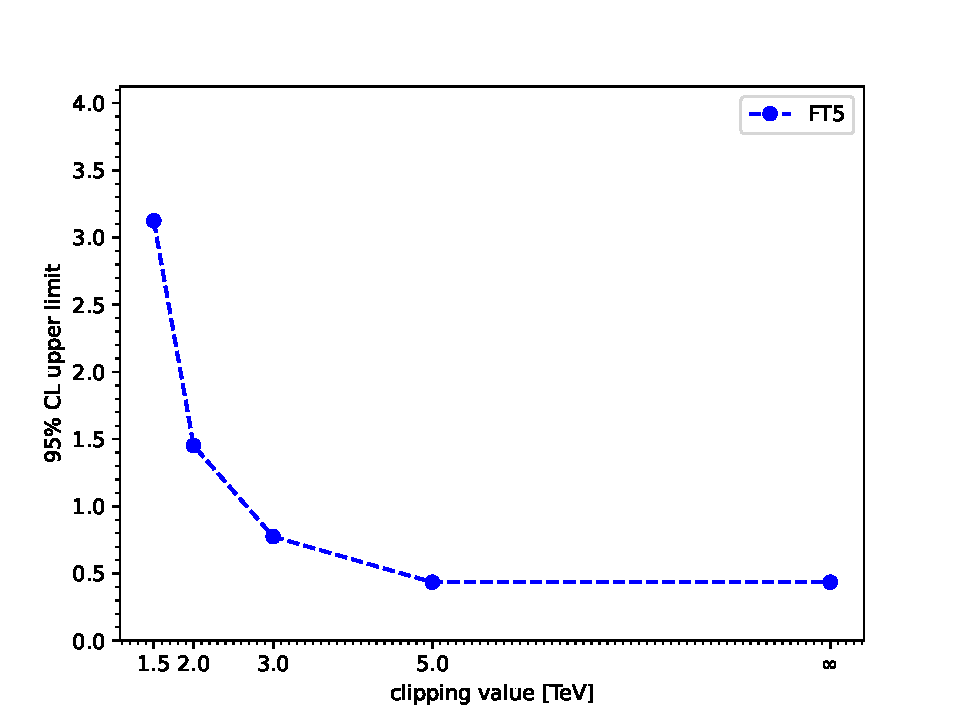
\includegraphics[width=0.35\textwidth]{figures/aQGC/ClippedFT5.pdf}
    	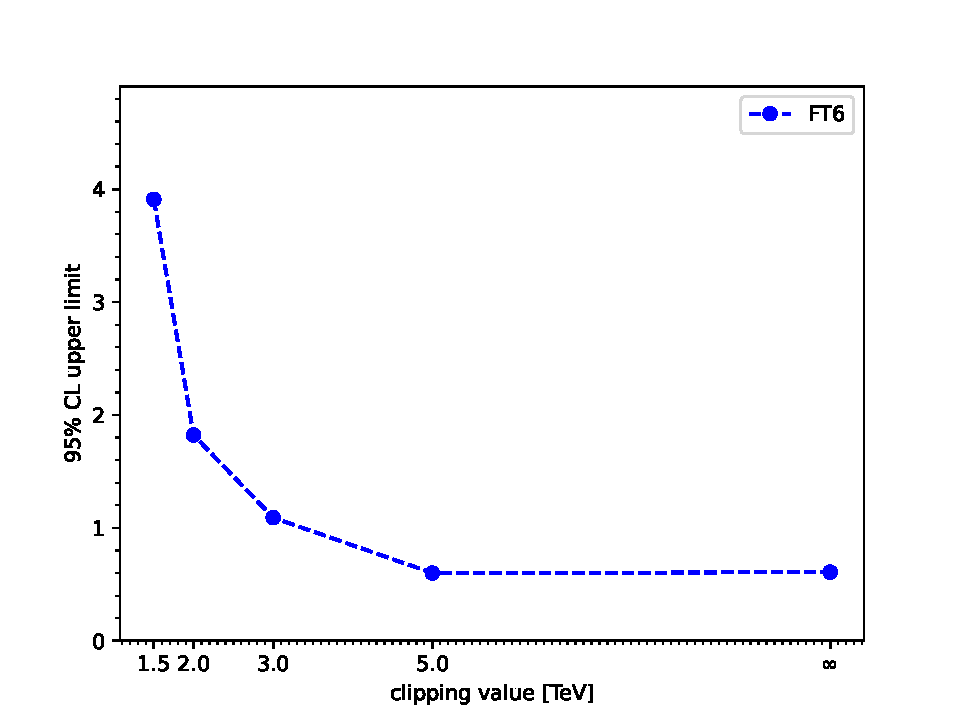
\includegraphics[width=0.35\textwidth]{figures/aQGC/ClippedFT6.pdf}
    	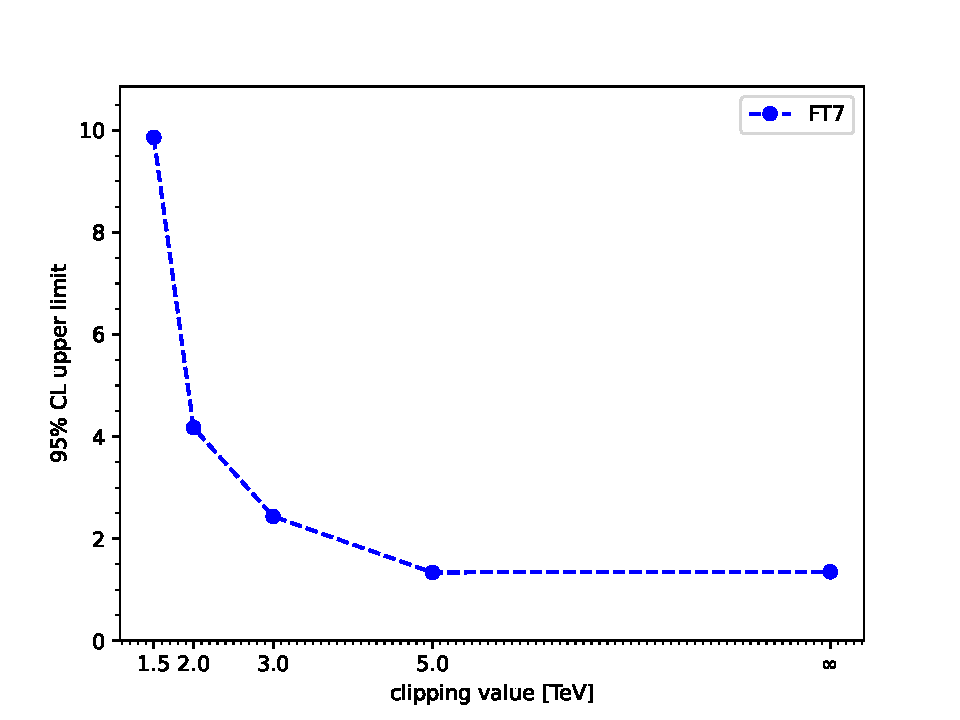
\includegraphics[width=0.35\textwidth]{figures/aQGC/ClippedFT7.pdf}
        \caption{Expected limits for 5 clipping points are shown for each coefficient FT5, FT6, and FT7.}
\end{figure}

\begin{figure}[ht]
    \centering
    	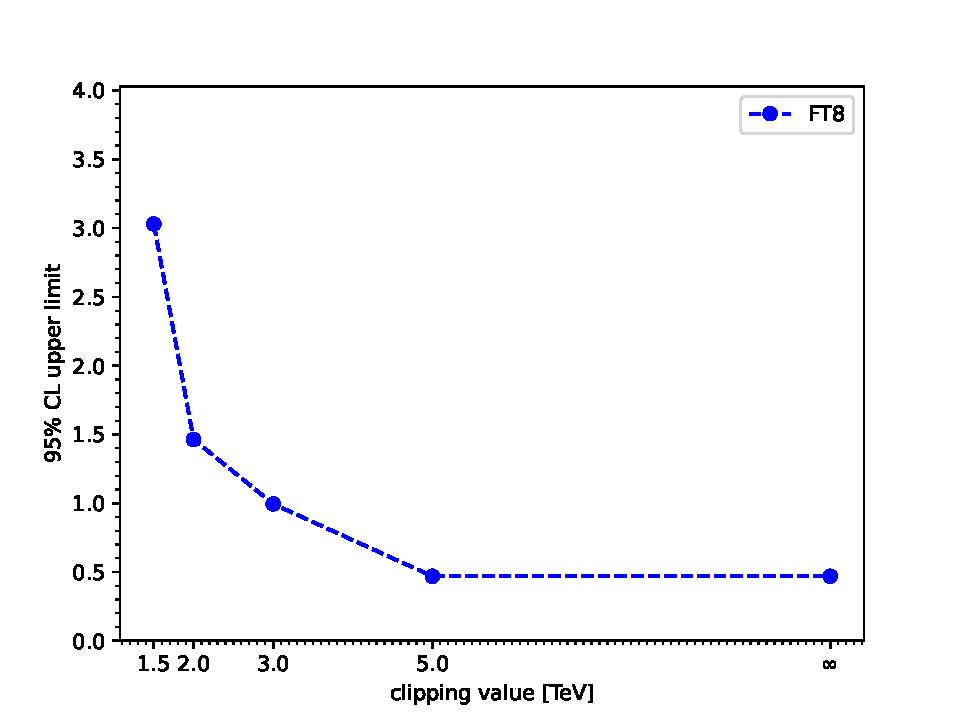
\includegraphics[width=0.35\textwidth]{figures/aQGC/ClippedFT8.pdf}
    	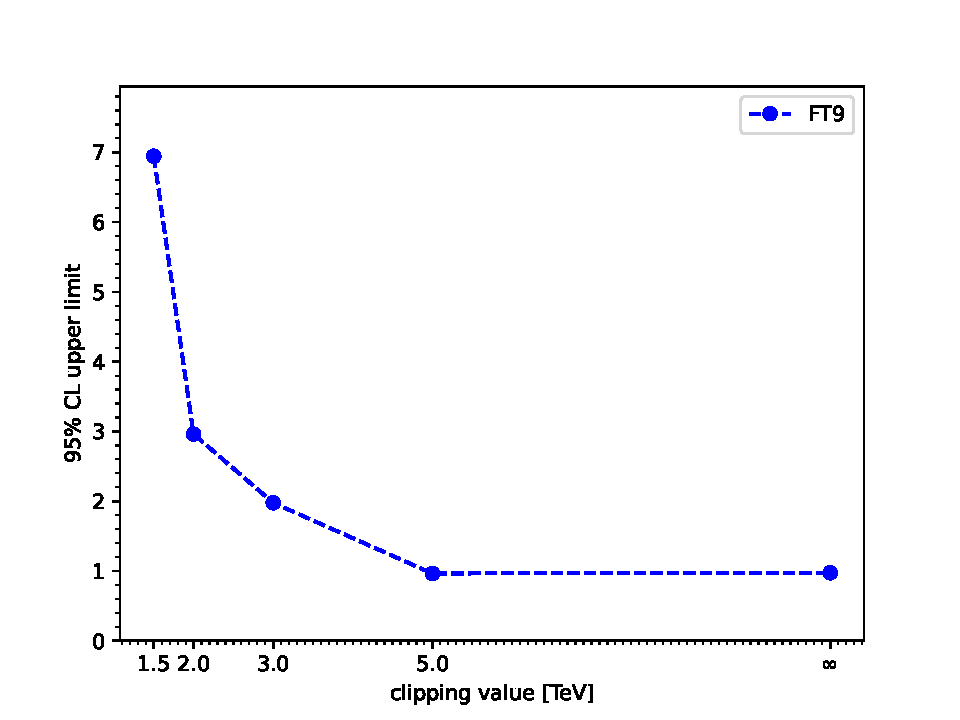
\includegraphics[width=0.35\textwidth]{figures/aQGC/ClippedFT9.pdf}
    	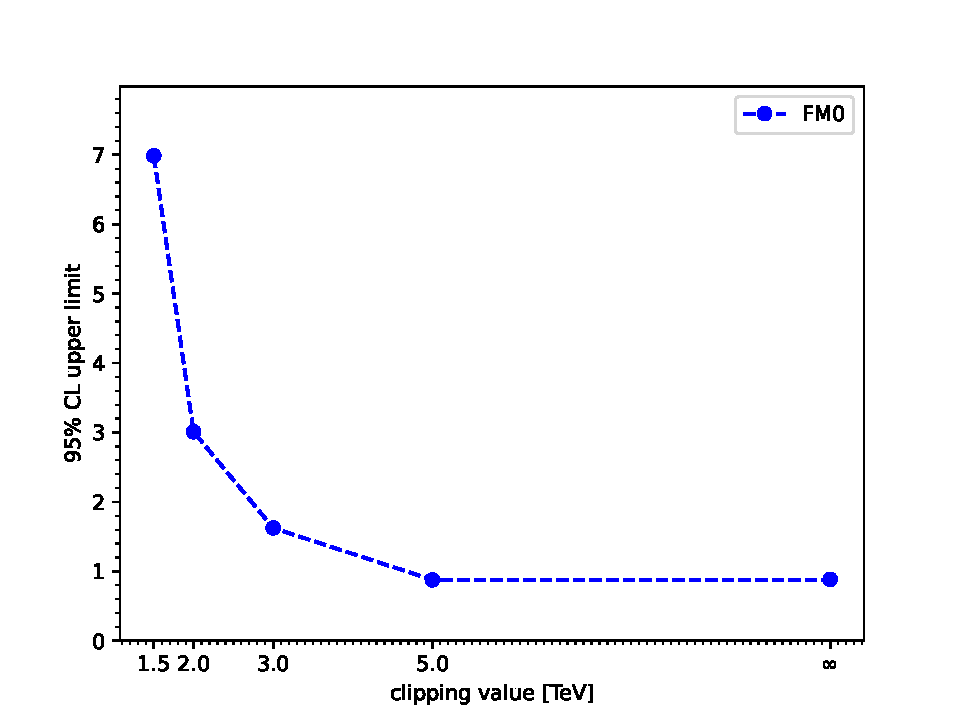
\includegraphics[width=0.35\textwidth]{figures/aQGC/ClippedFM0.pdf}
        \caption{Expected limits for 5 clipping points are shown for each coefficient FT8, FT9, and FM0.}
\end{figure}

\begin{figure}[ht]
    \centering
    	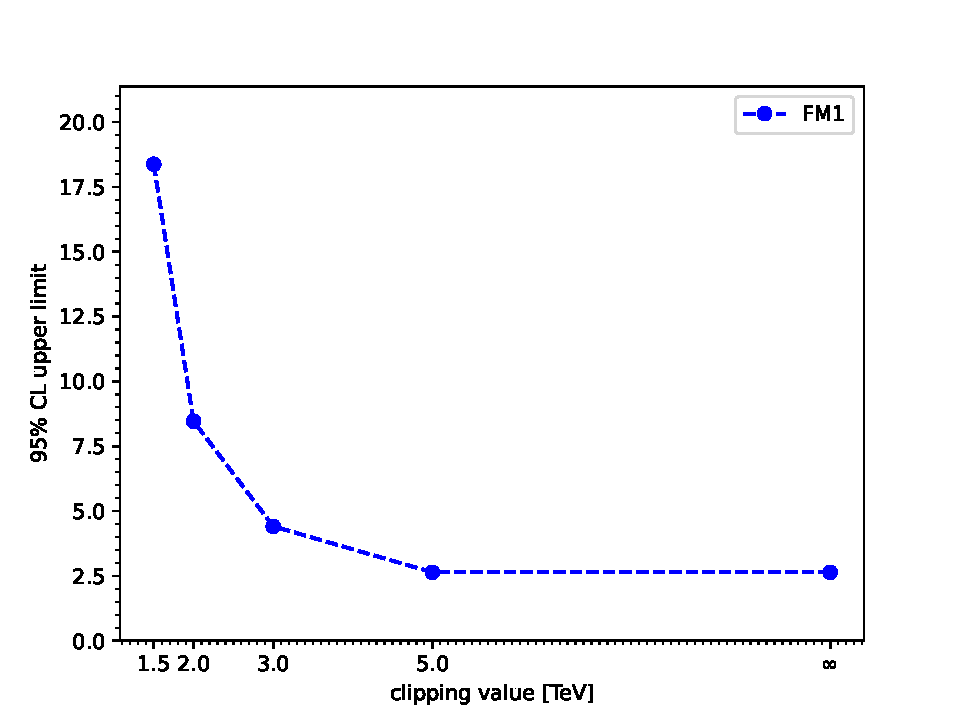
\includegraphics[width=0.35\textwidth]{figures/aQGC/ClippedFM1.pdf}
    	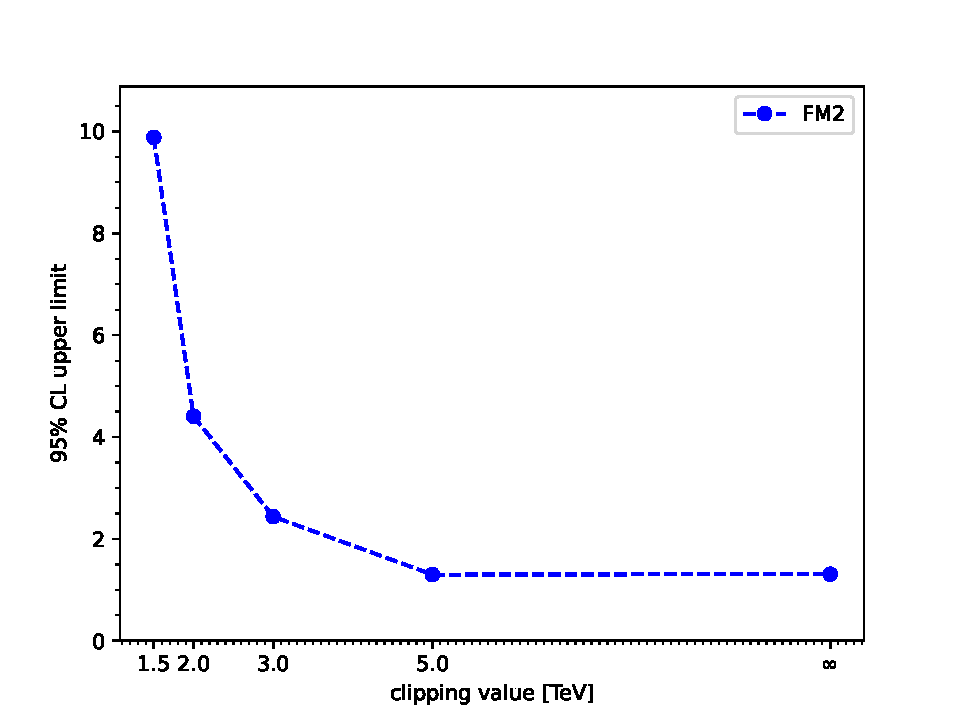
\includegraphics[width=0.35\textwidth]{figures/aQGC/ClippedFM2.pdf}
    	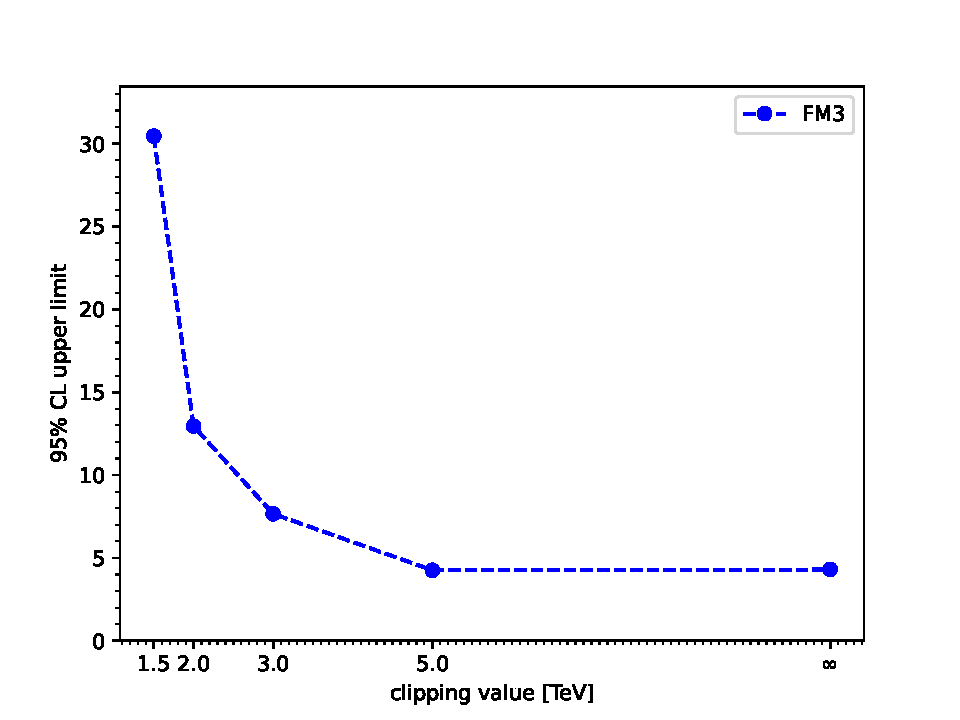
\includegraphics[width=0.35\textwidth]{figures/aQGC/ClippedFM3.pdf}
        \caption{Expected limits for 5 clipping points are shown for each coefficient FM1, FM2, and FM3.}
\end{figure}

\begin{figure}[ht]
    \centering
    	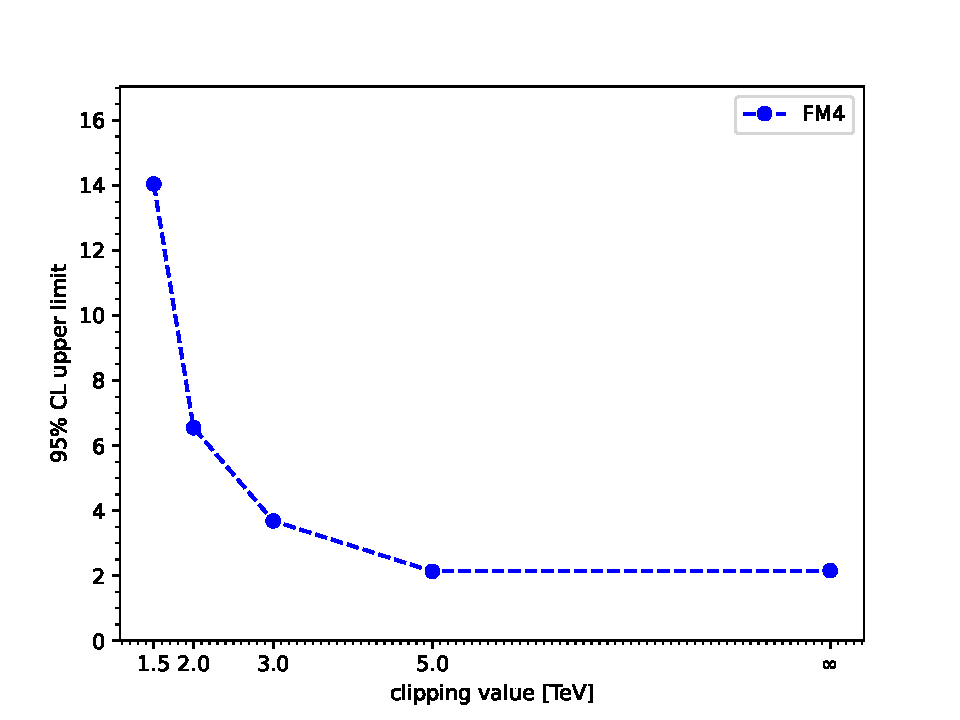
\includegraphics[width=0.35\textwidth]{figures/aQGC/ClippedFM4.pdf}
    	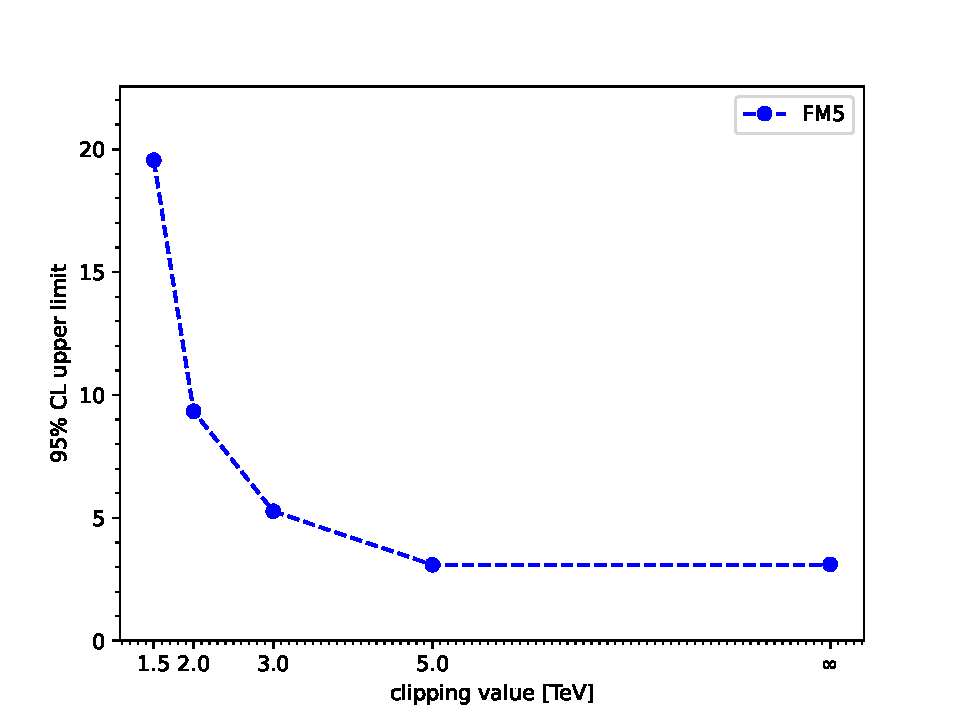
\includegraphics[width=0.35\textwidth]{figures/aQGC/ClippedFM5.pdf}
    	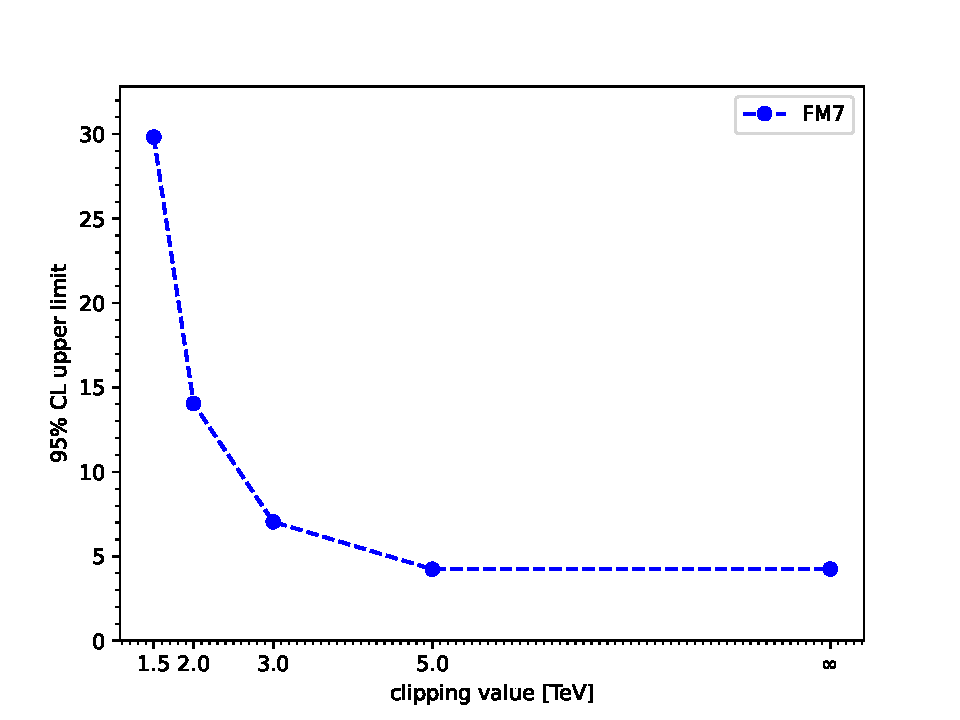
\includegraphics[width=0.35\textwidth]{figures/aQGC/ClippedFM7.pdf}
        \caption{Expected limits for 5 clipping points are shown for each coefficient FT4, FT5, and FM7.}
\end{figure}

\begin{figure}[ht]
    \centering
    	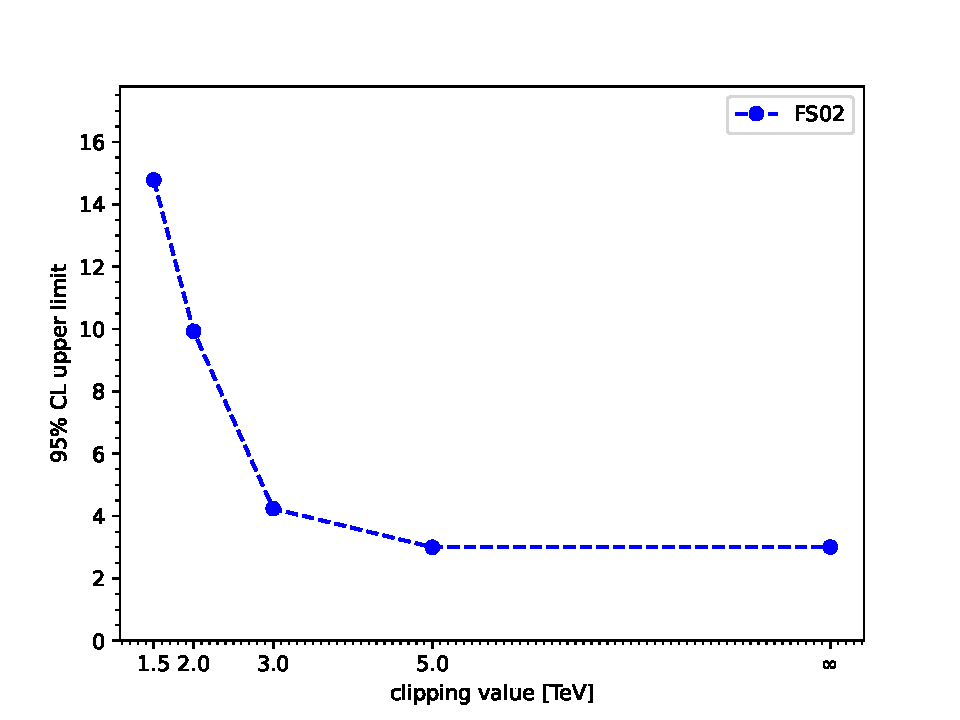
\includegraphics[width=0.35\textwidth]{figures/aQGC/ClippedFS02.pdf}
    	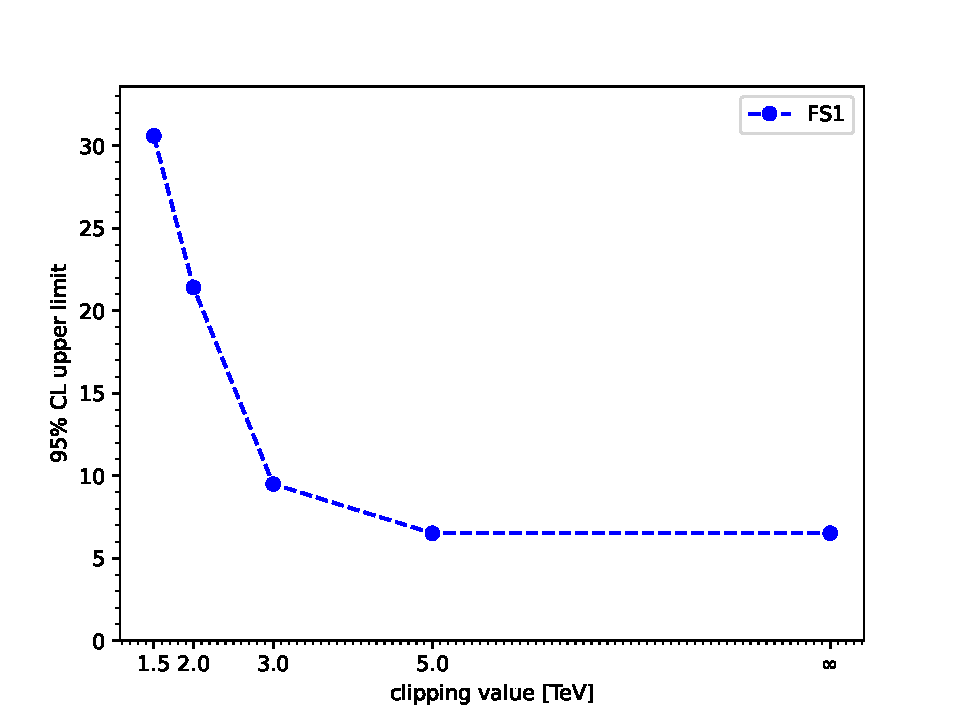
\includegraphics[width=0.35\textwidth]{figures/aQGC/ClippedFS1.pdf}
        \caption{Expected limits for 5 clipping points are shown for each cefficient FS02, FS1.}
\end{figure}

The expected limits for each Wilson coefficient is shown in the Table~\ref{}, in two cases. One is when the clipping value is 2~TeV and the other is when clipping value is $\infinity$, which means no clipping value is set.


\section{2-bin $m_{VV}$ approach}
\label{subsec:2binapproach}

There is a problem when we use the $m_{VV}$ distribution in the fit.
The normalization of the SM electroweak signal cannot be determined, since its shape is similar to the other background processes, as shown in Figure~\ref{fig:2lepaQGCshapeMVV}.
%RNN score shows the separation between standard model and the background, so the 2D fit of $m_{VV}$ and RNN score can be useful since we can use both separation powers. Spliting $m_{VV}$ in 2-bin is studied as the minimum case of 2D fit.

Unconditional asimov fit for FT0 signal in only \tlep channel is performed and compared in two options :
\begin{itemize}
  \item Fit $m_{VV}$ distribution as discriminant, as shown in section~\ref{subsec:aqgc_limit}
  \item Split the $m_{VV}$ into 2 bins ;  \\
        LowMVV : $m_{VV}$ $< 2000$~GeV \\
        HighMVV : $m_{VV}$ $\geq 2000$~GeV \\
        then fit simultaneously with RNN score as discriminant
\end{itemize}
Prefit plots are shown in figure~\ref{fig:2lepTwoBin} in the second option.
The expected limits and uncertainty of the expected signal strength of FT0 signal are shown in table~\ref{tab:2binlimit}.

\begin{figure}[ht]
    \centering
    	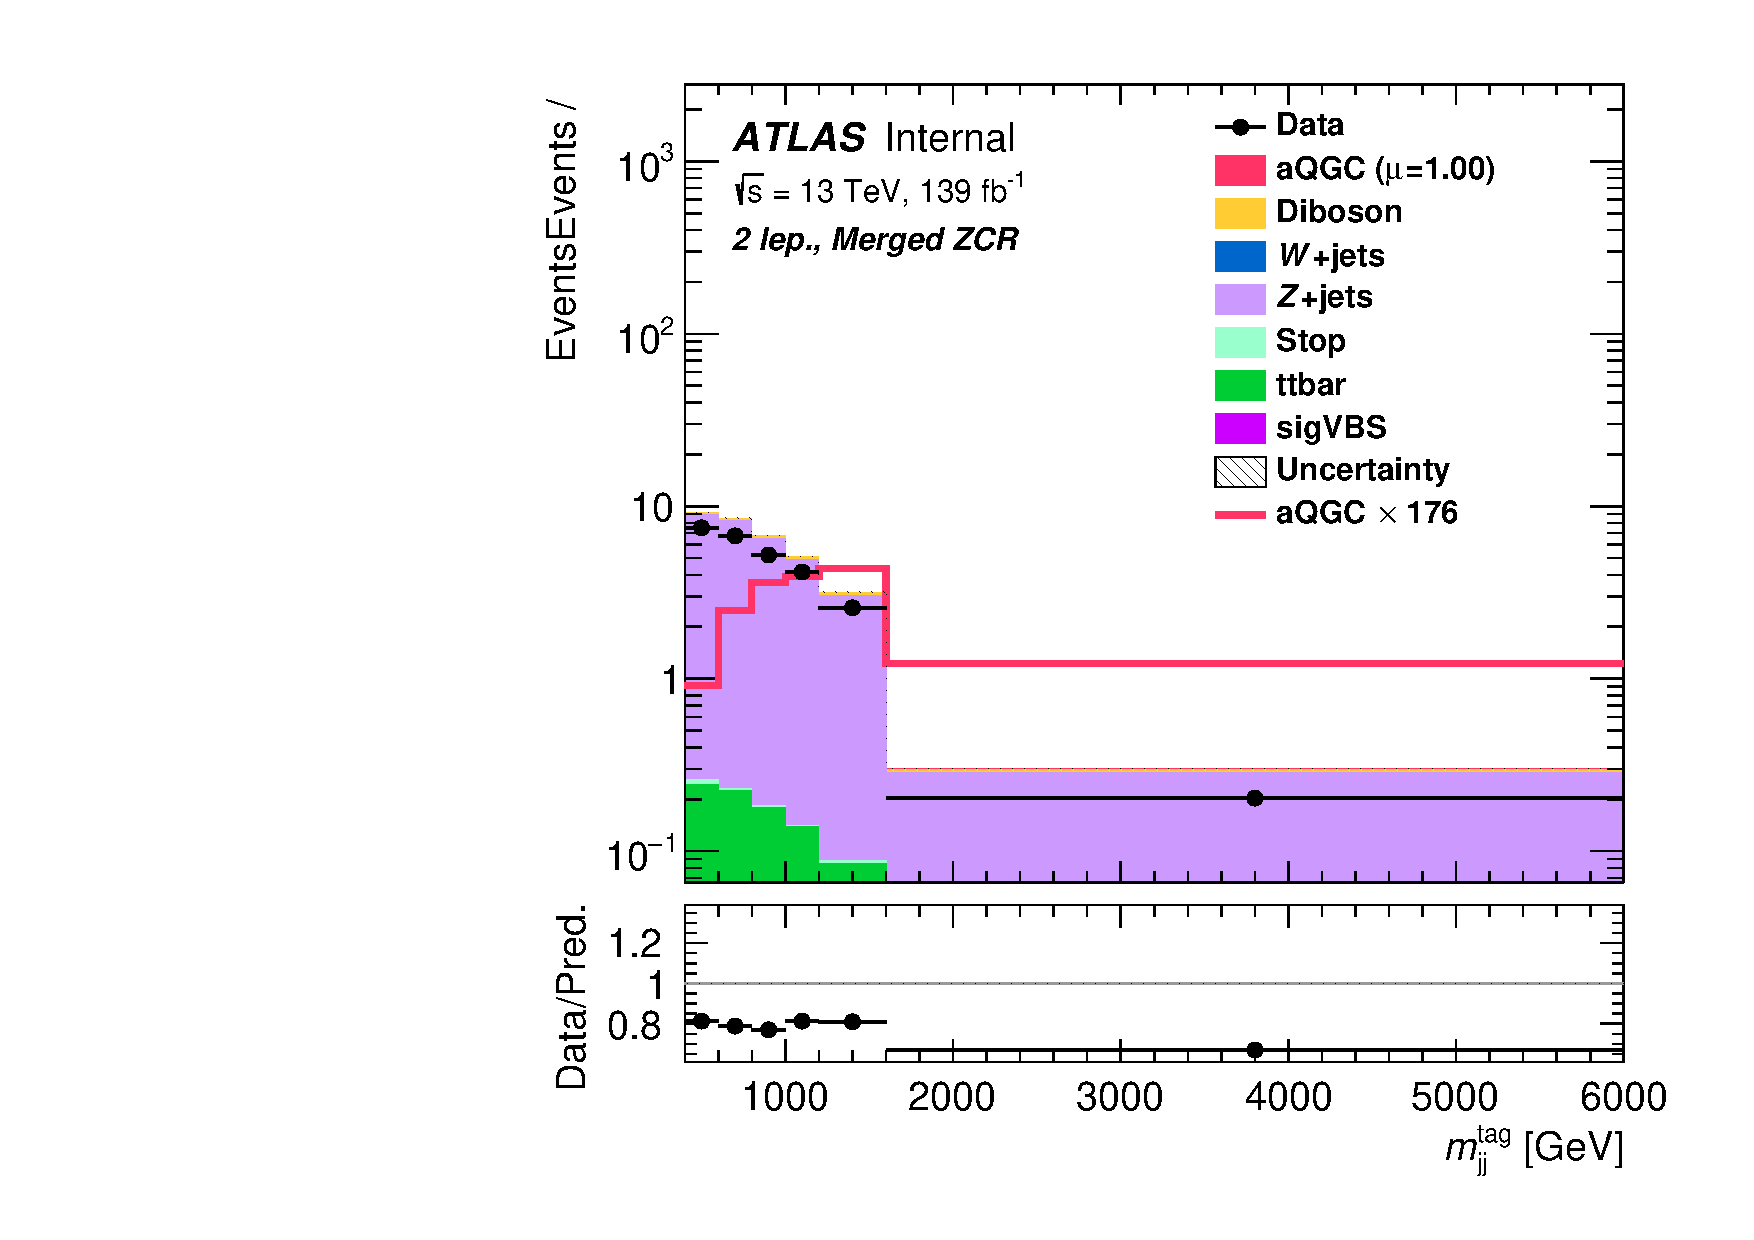
\includegraphics[width=0.35\textwidth]{figures/aQGC/Region_distMTagMerJets_DCRVjet_BMin0_J0_incJet1_L2_T0_incFat1_Y6051_incTag1_Fat1_Prefitlog.pdf}
    	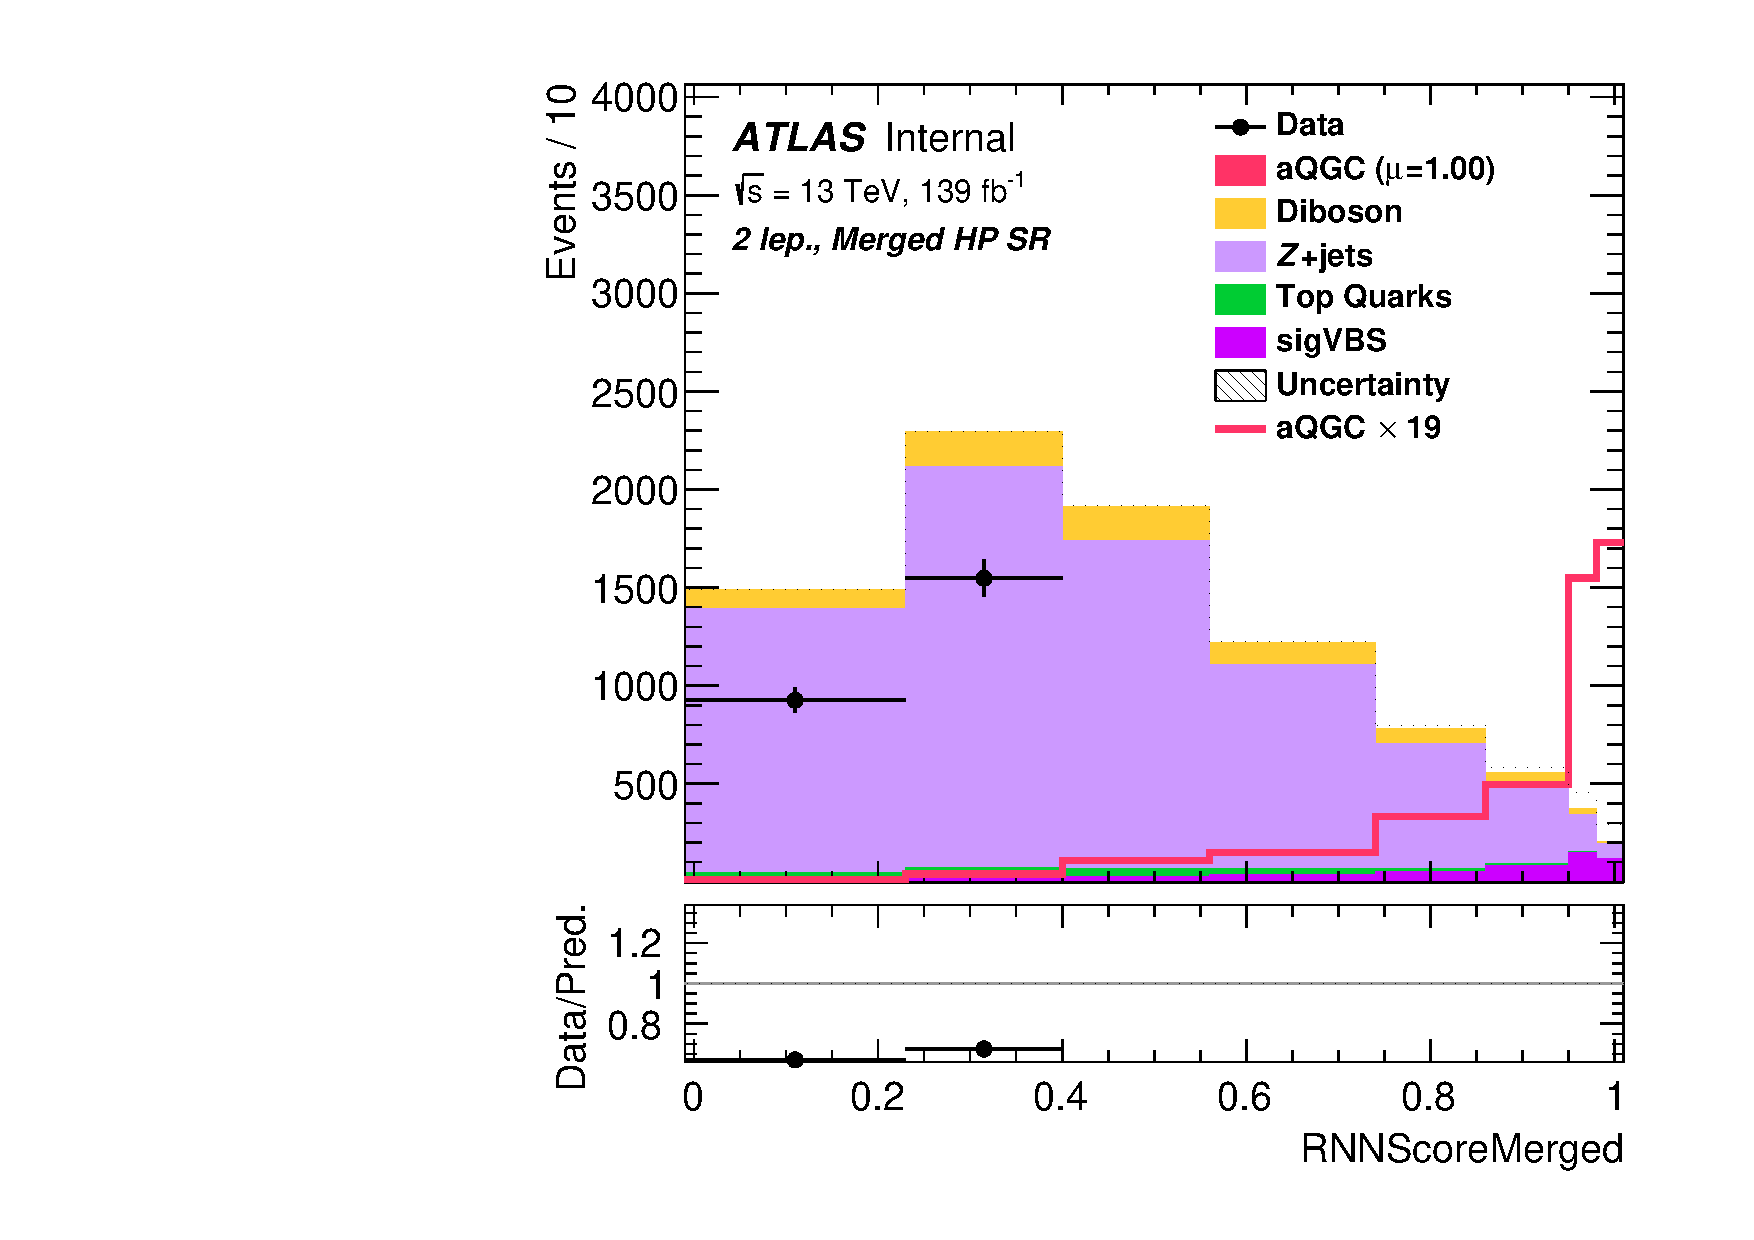
\includegraphics[width=0.35\textwidth]{figures/aQGC/Region_distRNNScoreMerged_DSRVBSHPLMVV_BMin0_J0_incJet1_L2_T0_incFat1_Y6051_incTag1_Fat1_Prefit.pdf}
    	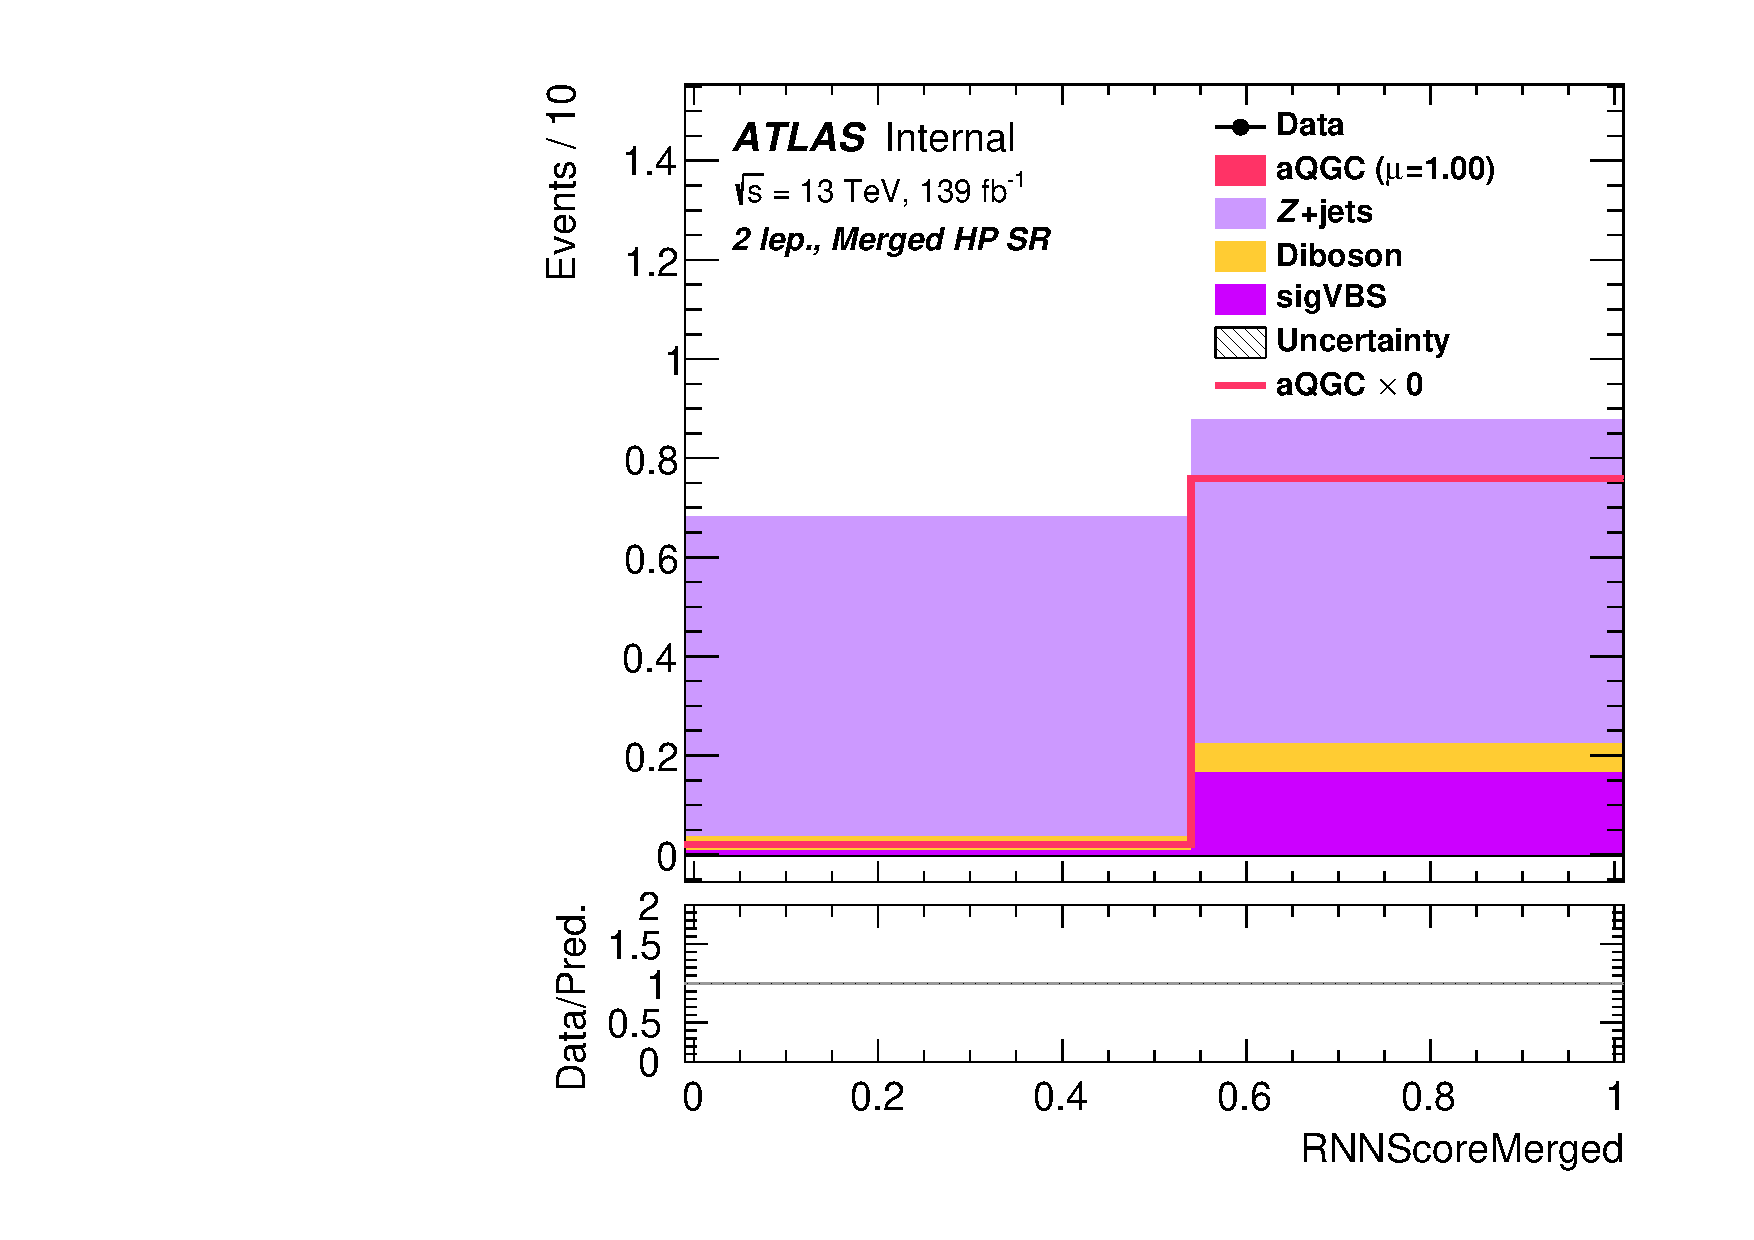
\includegraphics[width=0.35\textwidth]{figures/aQGC/Region_distRNNScoreMerged_DSRVBSHPHMVV_BMin0_J0_incJet1_L2_T0_incFat1_Y6051_incTag1_Fat1_Prefit.pdf}
    	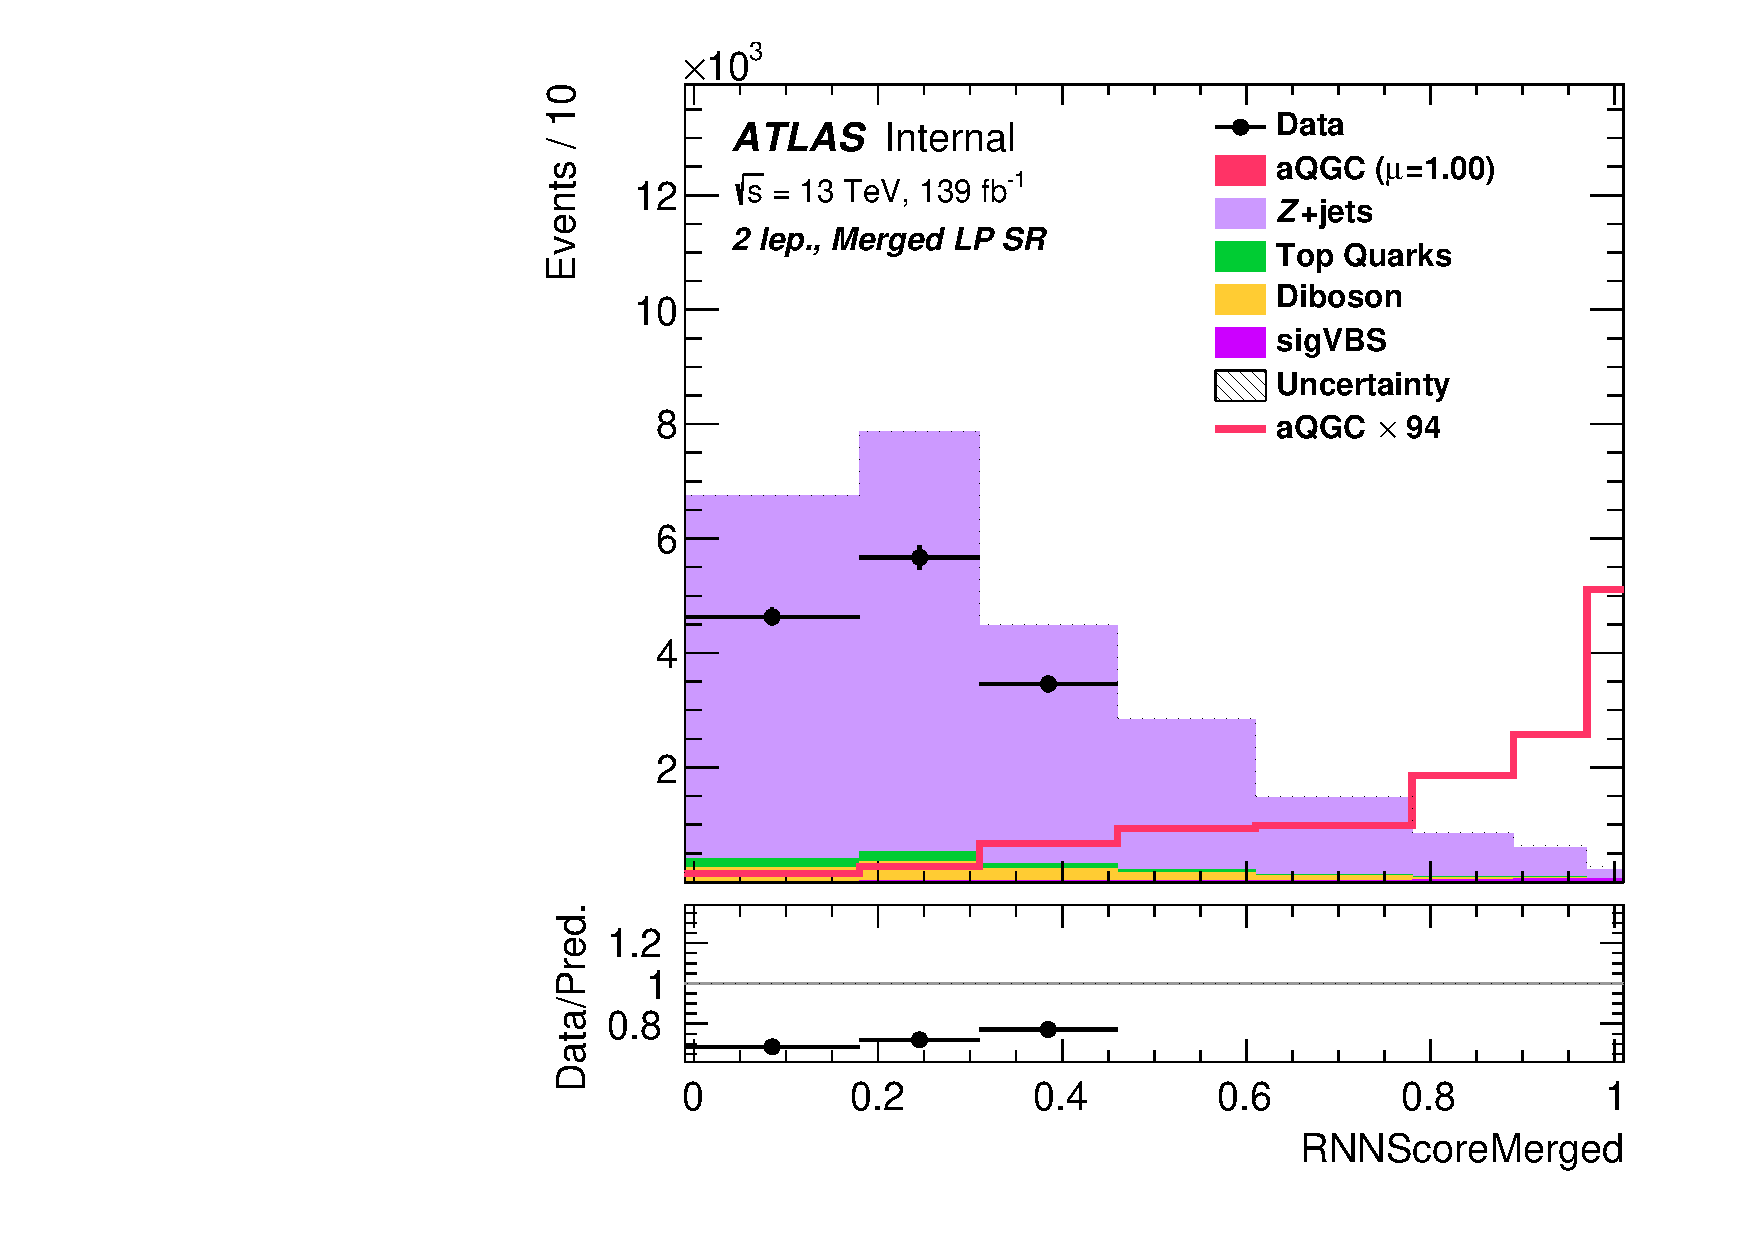
\includegraphics[width=0.35\textwidth]{figures/aQGC/Region_distRNNScoreMerged_DSRVBSLPLMVV_BMin0_J0_incJet1_L2_T0_incFat1_Y6051_incTag1_Fat1_Prefit.pdf}
    	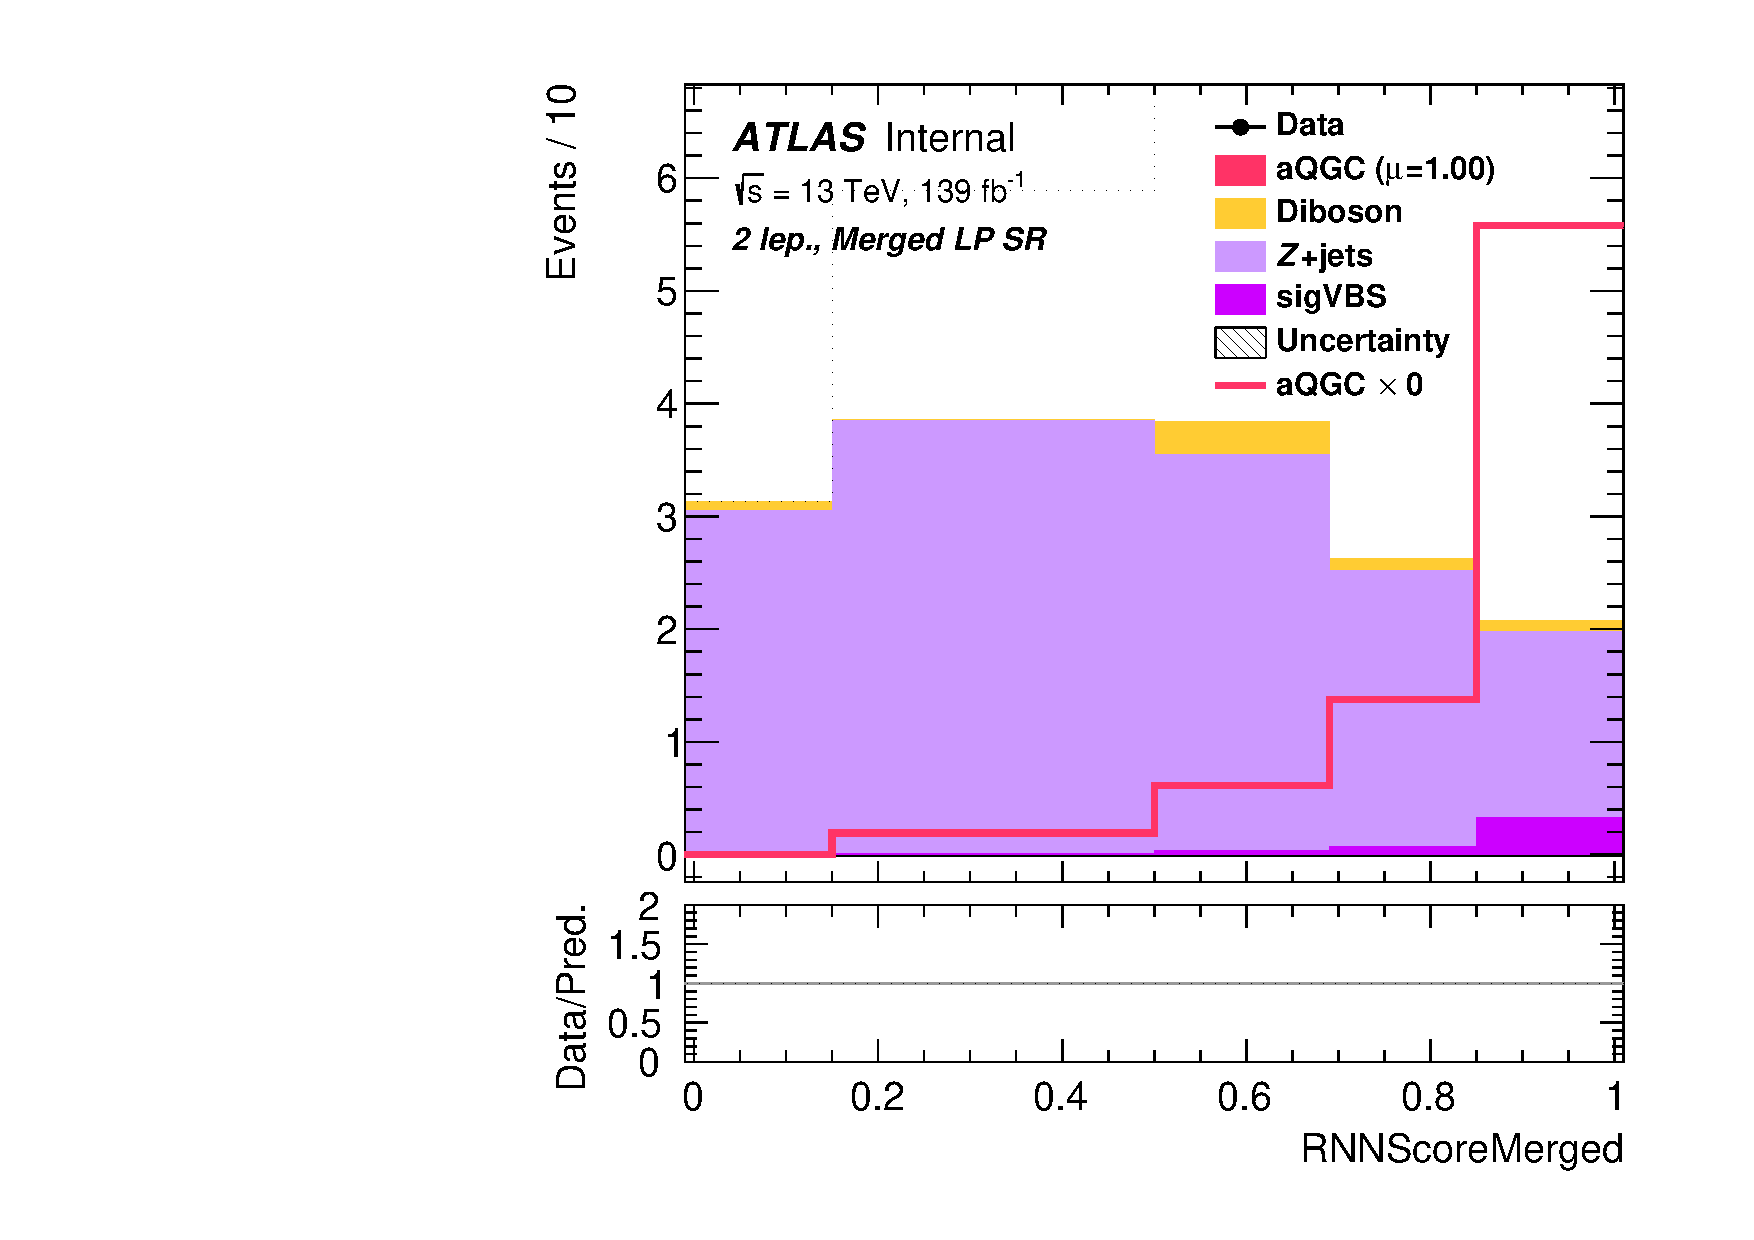
\includegraphics[width=0.35\textwidth]{figures/aQGC/Region_distRNNScoreMerged_DSRVBSLPHMVV_BMin0_J0_incJet1_L2_T0_incFat1_Y6051_incTag1_Fat1_Prefit.pdf}
        \caption{Prefit plots for 2-bin strategy is shown. The RNN score is used as discriminant for signal regions. operator FT0 in \tlep channel are shown. The standard model EW signal is floated as the background.}
        \label{fig:2lepTwoBin}
\end{figure}

\begin{table}[ht!]
\small
\begin{center}
\resizebox{0.9\textwidth}{!}{
\begin{tabular}{ | l || l | l | l |}
                                    & single bin fit with $m_{VV}$& single bin fit with RNN  & 2-bin fit with RNN   \tabularnewline \hline
Unconditional fitted $\mu$          & -2.7e-06 $\pm$ 0.067   & 3.38e-05 $\pm0.038$      & 3.35e-05 $\pm0.029$  \tabularnewline \hline
Norm sigVBS                         & 1 $\pm$ 2.1            & 1 $\pm$ 0.94             & 1 $\pm$ 0.48         \tabularnewline \hline
Norm Z                              & 1 $\pm$ 0.036          & 1 $\pm$ 0.029            & 1 $\pm$ 0.027        \tabularnewline \hline
Norm VV                             & 1 $\pm$ 1.13           & 1 $\pm$ 0.71             & 0.99 $\pm$ 0.64      \tabularnewline \hline
Expected limit of $\mu$             & 0.19                   & 0.72                     & 0.10                 \tabularnewline \hline
Expected limit of Wilson coefficient & 0.44                   & 0.85                     & 0.35                 \tabularnewline \hline
\end{tabular}
}
\caption{Expected signal strength and limits in each two options. only \tlep channel is used for the fit. The result for single bin fit with RNN is also shown as a reference. The normarizations fitted for standard model signal, and Z and diboson backgrounds are shown as Norm in the table.}
\label{tab:2binlimit}
\end{center}
\end{table}

2-bin fit can constrain the standard model signal, as shown in the uncertainty of Norm sigVBS of table~\ref{tab:2binlimit}. 
When comparing single bin fit with $m_{VV}$ and 2-bin fit with RNN, 2-bin fit with RNN appears to be able to provide a better limit.



